\documentclass[11pt]{article}

\usepackage[letterpaper,margin=0.82in]{geometry}
\usepackage[T1]{fontenc}
\usepackage[utf8]{inputenc}
\usepackage{lmodern}
\usepackage{microtype}
\usepackage{amsmath,amssymb,amsthm,mathtools}
\usepackage{booktabs,longtable,array}
\usepackage{enumitem}
\usepackage{xcolor}
\usepackage{hyperref}
\usepackage{fancyhdr}
\usepackage{listings}
\usepackage{graphicx}
\usepackage{float}
\usepackage{caption}
\captionsetup{font=small,labelfont=bf}
\graphicspath{{figures_final/}}

\hypersetup{
  colorlinks=true,
  linkcolor=blue!45!black,
  citecolor=blue!45!black,
  urlcolor=blue!45!black,
  pdftitle={Streaming Polyphase Factor Decomposition for SKAT-like Tests},
  pdfauthor={Komorebi P.}
}

\setlength{\parindent}{0pt}
\setlength{\parskip}{6pt}
\setlength{\headheight}{14pt}
\setlength{\emergencystretch}{2em}

\newtheorem{theorem}{Theorem}[section]
\newtheorem{proposition}[theorem]{Proposition}
\newtheorem{corollary}[theorem]{Corollary}
\newtheorem{lemma}[theorem]{Lemma}
\theoremstyle{definition}
\newtheorem{definition}[theorem]{Definition}
\newtheorem{algorithm}[theorem]{Algorithm}
\theoremstyle{remark}
\newtheorem{remark}[theorem]{Remark}

\pagestyle{fancy}
\fancyhf{}
\fancyhead[L]{Streaming Polyphase Factor Decomposition}
\fancyhead[R]{Komorebi P.}
\fancyfoot[C]{\thepage}

\title{\textbf{Streaming Polyphase Factor Decomposition for SKAT-like Quadratic-Form Tests}\\
\large Memory-Bounded Factor Actions, Phase-Local Krylov Structure, and Spectral Tail Compression}
\author{Komorebi P.}
\date{Illustrated manuscript v0.8 -- 2026-09-23}

\begin{document}
\maketitle

\begin{abstract}
Sequence kernel association testing (SKAT) is a variance-component framework for set-based rare-variant association testing \cite{Wu2011}. Large rare-variant and kernel tests often begin with a weighted factor
\[
A=M_XGW^{1/2},
\qquad
K=AA^\top,
\]
where \(G\in\mathbb R^{n\times m}\) is a genotype or feature matrix,
\(W\) is diagonal and nonnegative, and \(M_X\) projects away null-model
covariates.  When \(m\) is large, the direct factor \(A\) may exceed device
memory even though the final statistic requires only a spectrum or repeated
operator actions.  This manuscript formalizes a composable decomposition
calculus with four independent layers: storage blocks, structural
polyphase packets, Krylov/range compression, and final spectral packets for
deep-tail evaluation.  The core exact result is that both \(K\) and every
Krylov action can be evaluated by streaming variant blocks, so total variant
count controls arithmetic and I/O but need not control device working-set
size.  Storage refinement is proved invariant, two-dimensional sample/variant
tiling is exact, and the streaming layer composes with an exact polyphase
light-cone theorem, minimal phase-local rank allocation, low-rank interface
messages, and exact QR-core updates.  When phase couplings are weak rather
than zero, a nonnegative transfer matrix gives certified phasewise leakage
bounds for operator powers and complete Krylov polynomials.  A dual
query/spectral budget propagates pruning uncertainty to generalized-\(\chi^2\)
tail brackets, while residual trace, square-trace, and spectral-cap invariants
supply substantially sharper incomplete-range certificates and an exact
moment-triggered residual-completion rule.
Reference implementations reproduce
explicitly formed operators to roughly machine precision.  For
\(n=2000\), Krylov width \(16\), covariate rank \(4\), and resident variant
block \(1024\), the algebraic streamed kernel-action working set is about
\(16.3\) MiB and remains constant from \(m=10^4\) through \(m=10^6\), while
the full float64 factor grows from about \(153\) MiB to \(15.3\) GiB.
\end{abstract}

\tableofcontents
\clearpage

\section{Problem and decomposition axes}

Let
\[
G\in\mathbb R^{n\times m},
\qquad
W=\operatorname{diag}(w_1,\ldots,w_m),
\quad w_j\ge 0,
\]
and let \(Q_X\in\mathbb R^{n\times p}\) have orthonormal columns spanning
the null-model covariates.  Define
\[
M_X=I-Q_XQ_X^\top,
\qquad
A=M_XGW^{1/2},
\qquad
K=AA^\top.
\]

The central implementation difficulty is not the algebraic size of the
model but the mismatch between the total factor size \(n\times m\) and the
working memory of an accelerator.  The key point of this manuscript is that
several decompositions act on different mathematical coordinates and therefore
compose:
\[
\boxed{
\text{storage blocks}
\circ
\text{structural phases}
\circ
\text{Krylov/range compression}
\circ
\text{spectral tail packets}.
}
\]

Storage blocking controls residence.  Structural phases encode LD windows,
annotations, frequency bands, or other coordinate groups.  Krylov methods
compress the operator to the rank actually requested.  Spectral packets
compress the final generalized-\(\chi^2\) transform.


\begin{figure}[H]
\centering
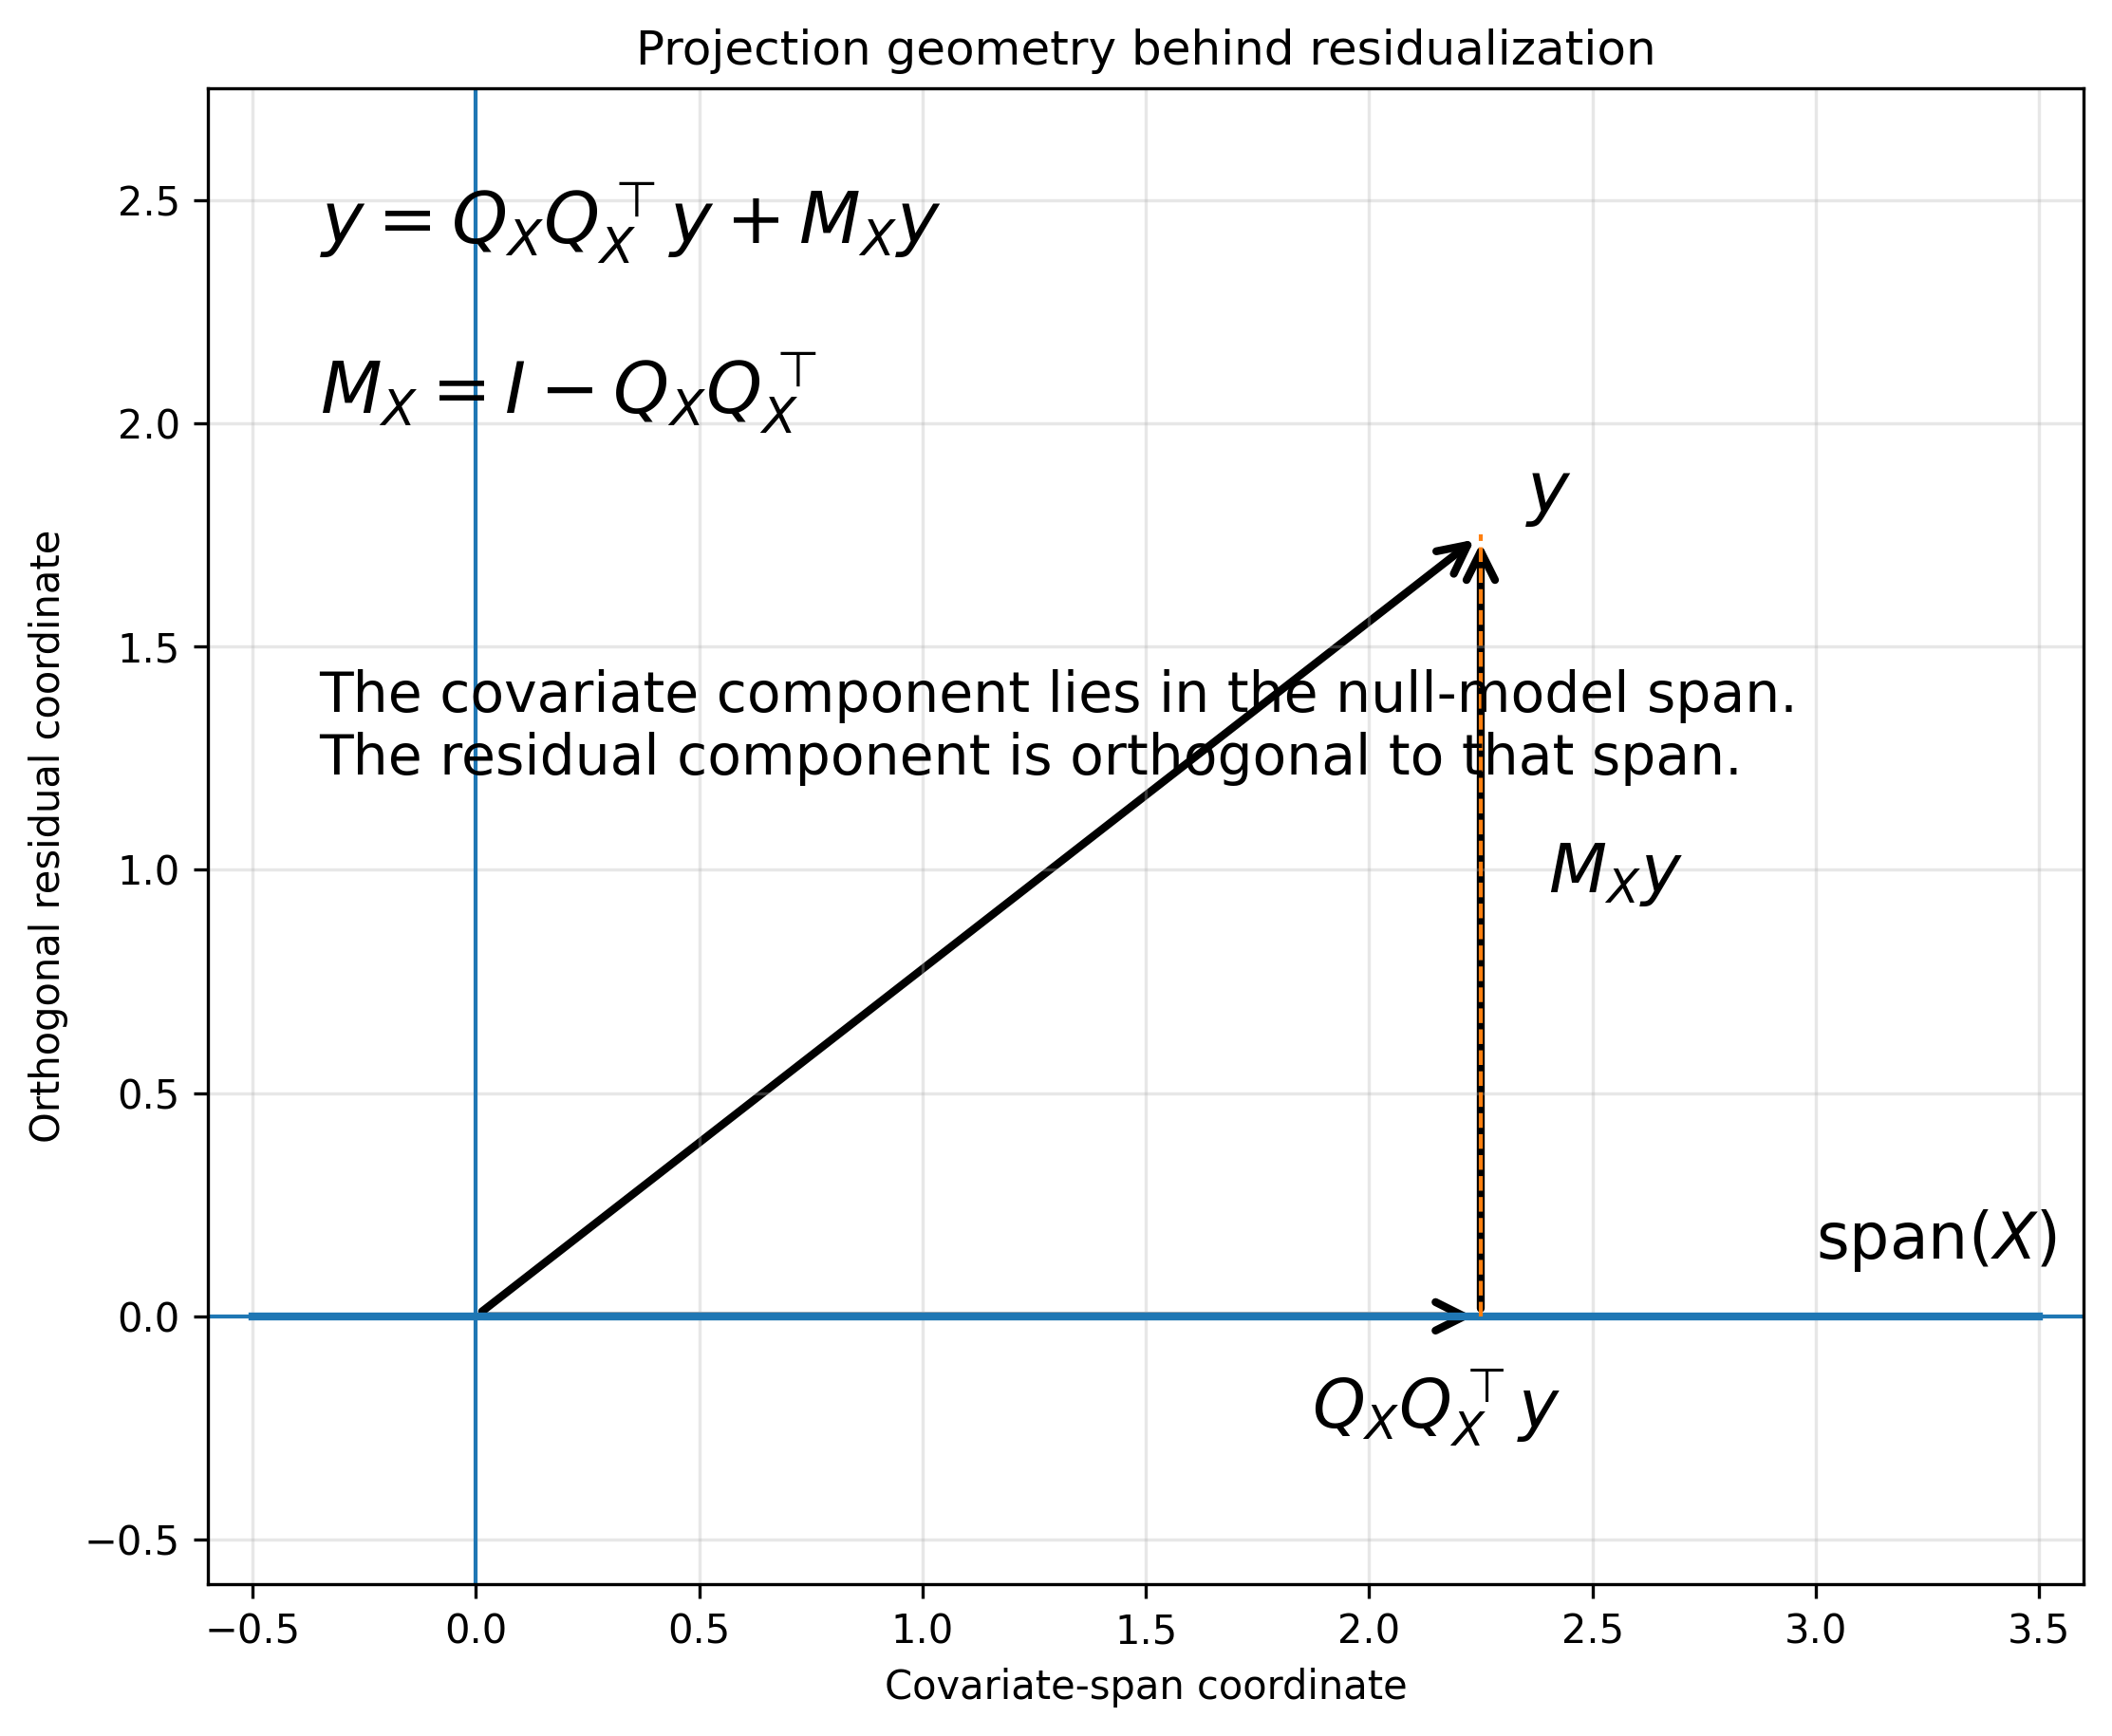
\includegraphics[width=.72\linewidth]{figure_01_residualization_geometry.png}
\caption{Residualization is the geometric starting point. Every sample-space vector splits into a component in the covariate span and an orthogonal residual component. The factor $A=M_XGW^{1/2}$ therefore acts only on variation remaining after the null-model covariates have been removed.}
\label{fig:residualization-geometry}
\end{figure}

\section{Variant-block Gram decomposition}

Partition the variant indices into disjoint blocks
\[
\{1,\ldots,m\}
=
J_1\sqcup\cdots\sqcup J_B.
\]
Let
\[
G_b=G_{[:,J_b]},
\qquad
W_b=W_{J_b,J_b},
\qquad
A_b=M_XG_bW_b^{1/2}.
\]
Then
\[
A=[A_1\ \cdots\ A_B].
\]

\begin{theorem}[Additive block Gram identity]
\[
\boxed{
K
=
AA^\top
=
\sum_{b=1}^B A_bA_b^\top
=
M_X
\left(
\sum_{b=1}^B G_bW_bG_b^\top
\right)
M_X.
}
\]
\end{theorem}

\begin{proof}
Horizontal concatenation gives
\[
[A_1\ \cdots\ A_B]
\begin{bmatrix}
A_1^\top\\
\vdots\\
A_B^\top
\end{bmatrix}
=
\sum_bA_bA_b^\top.
\]
The final form follows from
\(A_b=M_XG_bW_b^{1/2}\) and
\(M_X^\top=M_X=M_X^2\).
\end{proof}

\begin{remark}
The theorem is exact for every partition.  Block boundaries are execution
parameters, not statistical parameters.
\end{remark}


\begin{figure}[H]
\centering
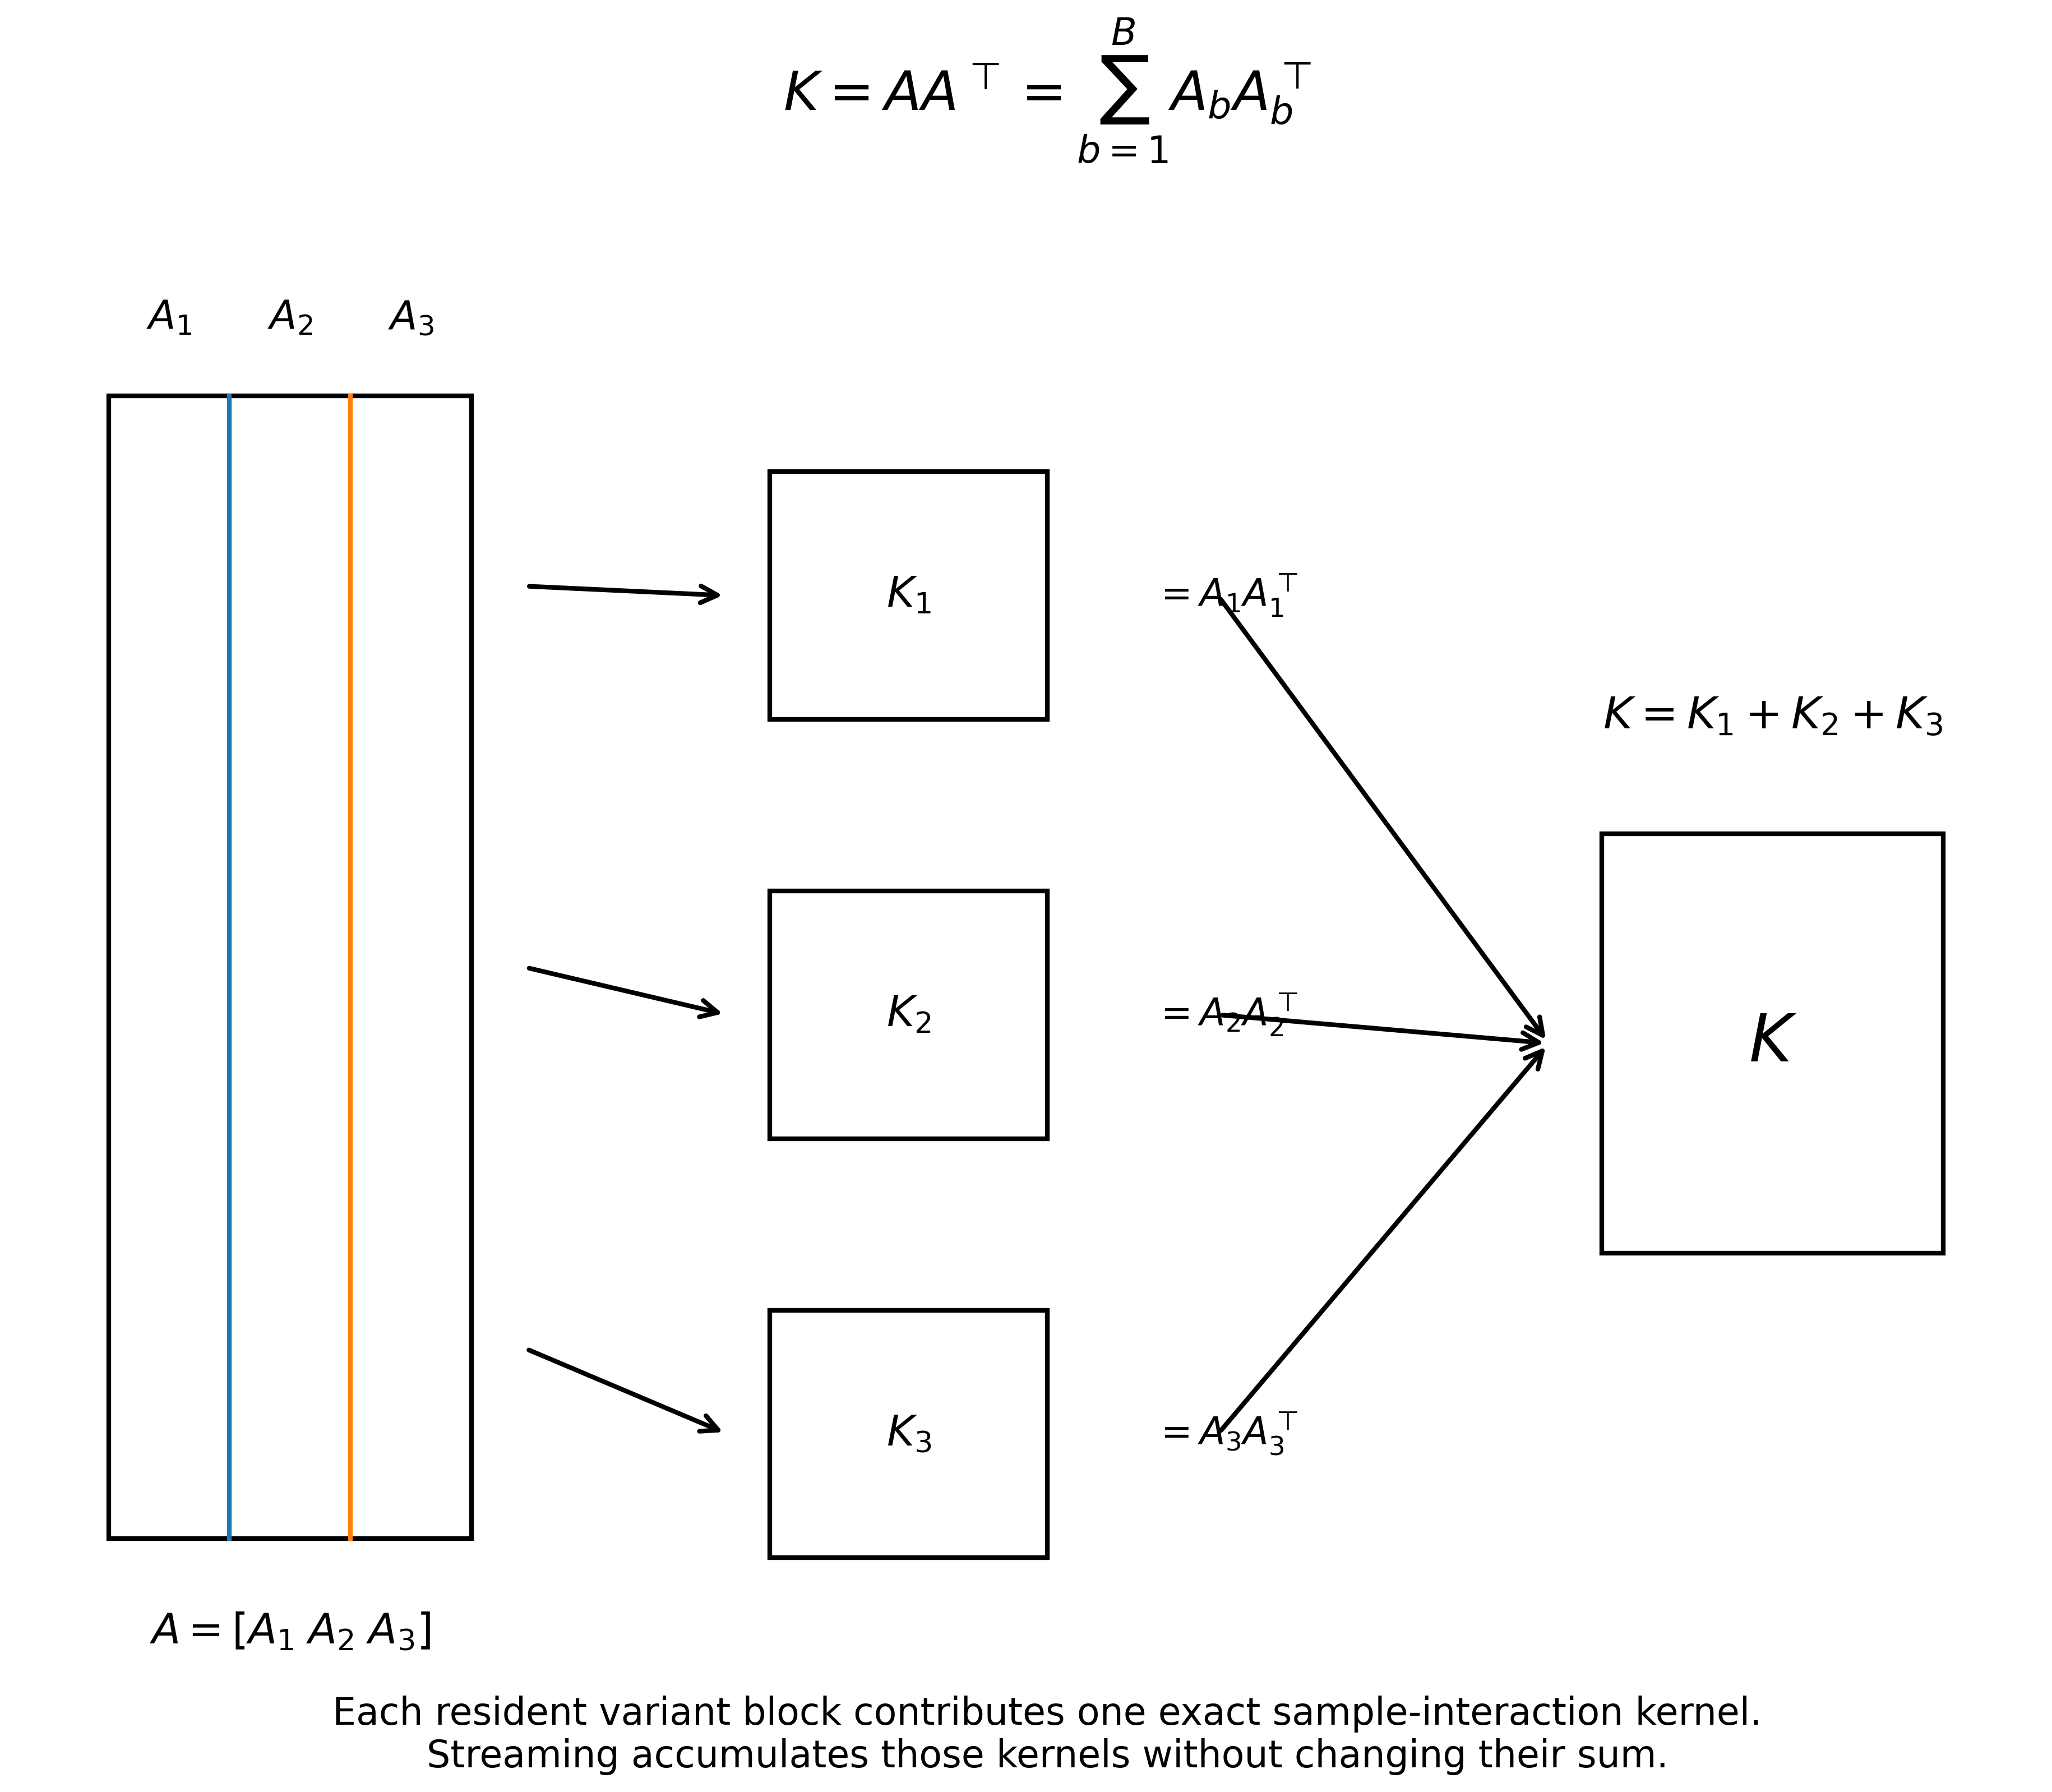
\includegraphics[width=.92\linewidth]{figure_02_exact_block_kernel_assembly.png}
\caption{Exact block-kernel assembly. The sample interaction kernel carried by each resident variant block is $K_b=A_bA_b^\top$, and the full kernel is their exact sum. Streaming changes the order of evaluation, not the operator.}
\label{fig:block-kernel-assembly}
\end{figure}

\section{Exact streamed kernel actions}

\begin{theorem}[One-pass sample-space streaming action]
For every block vector \(V\in\mathbb R^{n\times s}\),
\[
\boxed{
KV
=
M_X
\sum_{b=1}^B
G_bW_bG_b^\top
M_XV.
}
\]
\end{theorem}

\begin{proof}
Apply the additive block Gram identity to \(KV\), then associate each block
product as
\[
G_bW_b(G_b^\top M_XV).
\]
\end{proof}

\begin{algorithm}[Streamed \(KV\)]
\begin{enumerate}[label=\arabic*.]
\item Compute \(U=M_XV\).
\item Set \(Y=0\).
\item For each resident block \(b\), compute
\[
T_b=G_b^\top U,
\qquad
Y\leftarrow Y+G_b(W_bT_b).
\]
\item Return \(M_XY\).
\end{enumerate}
\end{algorithm}

\begin{corollary}[Working memory independent of total variant count]
If at most \(c\) variants are resident and the block-vector width is \(s\),
then the algebraic working set is
\[
\boxed{
O(nc+ns+cs+np),
}
\]
independent of total variant count \(m\).
\end{corollary}

\section{Streamed factor actions and Golub--Kahan}

Let \(V\in\mathbb R^{m\times s}\) be partitioned conformally:
\[
V=
\begin{bmatrix}
V_1\\
\vdots\\
V_B
\end{bmatrix}.
\]

\begin{theorem}[Streamed \(AV\)]
\[
\boxed{
AV
=
M_X
\sum_{b=1}^B
G_bW_b^{1/2}V_b.
}
\]
\end{theorem}

\begin{theorem}[Streamed \(A^\top U\)]
For \(U\in\mathbb R^{n\times s}\),
\[
\boxed{
(A^\top U)_b
=
W_b^{1/2}G_b^\top M_XU.
}
\]
\end{theorem}

\begin{proof}
Both identities follow by substituting
\(A=M_XGW^{1/2}\) and partitioning the variant coordinate.
\end{proof}

\begin{corollary}[Streaming Golub--Kahan equivalence]
Any exact-arithmetic algorithm whose access to \(A\) occurs only through
\(AV\) and \(A^\top U\) produces the same iterates when those products are
implemented by the preceding streamed formulas.
\end{corollary}

This applies directly to block Golub--Kahan bidiagonalization, matrix-free
singular-value iteration, range finding, and restarted variants.  The
factor need not be resident.

\section{Two-pass dual action}

The variant-space normal operator is
\[
H=A^\top A.
\]

\begin{theorem}[Two-pass streamed dual action]
For every \(V\in\mathbb R^{m\times s}\),
\[
\boxed{
HV=A^\top(AV).
}
\]
The product is evaluated exactly by a streamed pass forming
\(Y=AV\in\mathbb R^{n\times s}\), followed by a second streamed pass
emitting the blocks
\[
(HV)_b=W_b^{1/2}G_b^\top M_XY.
\]
\end{theorem}

This form is particularly natural for variant-space polyphase Krylov
iterations because the right-coordinate blocks can be produced and consumed
sequentially.

\section{Two-dimensional sample/variant tiling}

A variant block may itself exceed device memory.  Let
\[
H_b=G_bW_b^{1/2}
\]
and partition samples into row tiles \(I_1,\ldots,I_R\).

\begin{theorem}[Two-pass residualized tile construction]
Define
\[
R_b=Q_X^\top H_b.
\]
Then
\[
\boxed{
R_b
=
\sum_r
Q_{X,I_r}^\top H_{b,I_r},
}
\]
and after \(R_b\) is known,
\[
\boxed{
A_{b,I_r}
=
H_{b,I_r}-Q_{X,I_r}R_b.
}
\]
Consequently,
\[
\boxed{
K_{I_r,I_s}
=
\sum_b
A_{b,I_r}A_{b,I_s}^\top.
}
\]
\end{theorem}

\begin{proof}
The first identity is the row-partitioned matrix product
\(Q_X^\top H_b\).  The second is the definition
\(M_XH_b=H_b-Q_XQ_X^\top H_b\).  The last identity is the corresponding
sample-tile expansion of \(AA^\top\).
\end{proof}

With sample tile height \(t\) and resident variant width \(c\), the dominant
working storage is
\[
O(tc+pc+t^2).
\]

\section{Partition refinement and permutation invariance}

\begin{theorem}[Partition-refinement invariance]
Let \(\mathcal J\) be any partition of the variants and let
\(\mathcal J'\) refine \(\mathcal J\).  Then
\[
\boxed{
\sum_{J\in\mathcal J}A_JA_J^\top
=
\sum_{J'\in\mathcal J'}A_{J'}A_{J'}^\top
=
AA^\top.
}
\]
The analogous streamed operator action is also invariant.
\end{theorem}

\begin{proof}
Each coarse block is a disjoint union of refined blocks.  Apply the additive
Gram theorem within each coarse block and sum.
\end{proof}

\begin{corollary}[Adaptive memory splitting]
A runtime may recursively subdivide any block that exceeds available device
memory without changing the exact operator.
\end{corollary}

\begin{proposition}[Variant permutation invariance]
If the columns of \(G\) and the diagonal entries of \(W\) are permuted by the
same permutation, \(K\) and every streamed sample-space action are unchanged.
\end{proposition}


\begin{figure}[H]
\centering
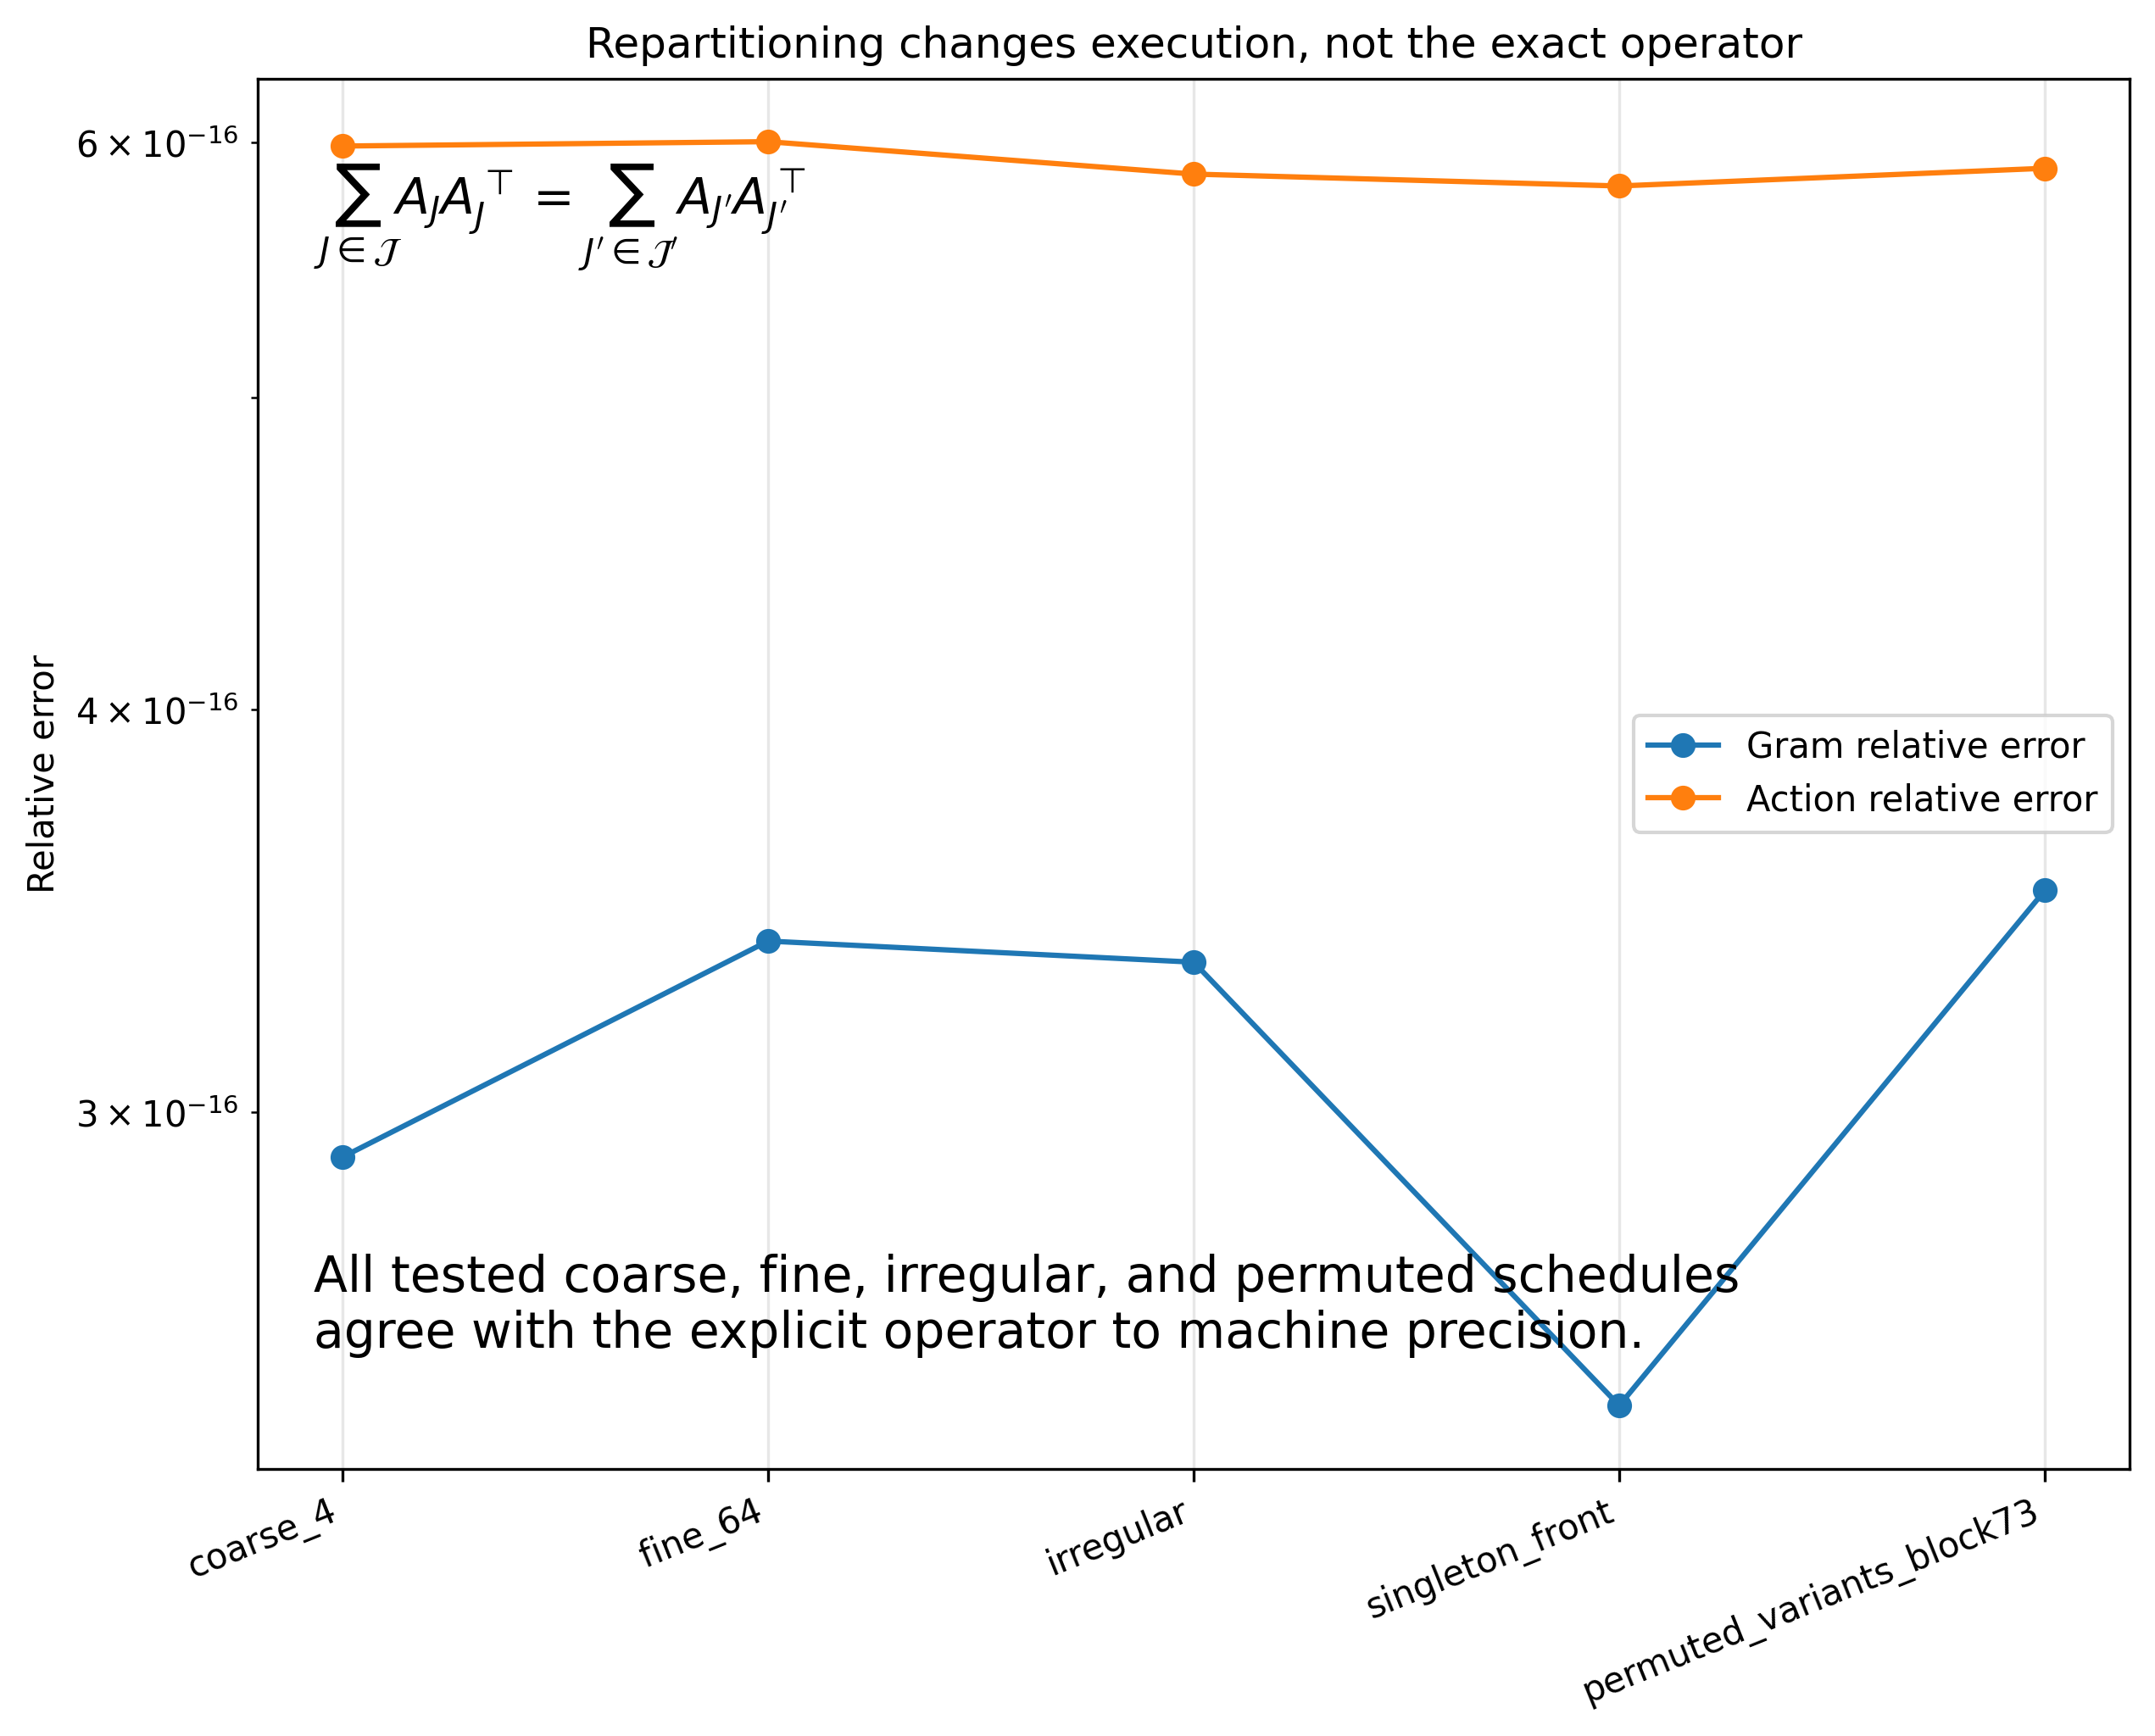
\includegraphics[width=.84\linewidth]{figure_08_partition_invariance.png}
\caption{Partition-refinement invariance in floating-point tests. Coarse, fine, irregular, singleton-heavy, and permuted blockings reproduce the explicitly formed Gram matrix and its action to machine precision. The block schedule is therefore an execution choice rather than a change in the statistical model.}
\label{fig:partition-invariance}
\end{figure}

\section{Polyphase structure}

Let \(P_h\) project onto variant phase \(h\), and again set
\[
H=A^\top A.
\]
Define the exact phase graph by
\[
g\to h
\quad\Longleftrightarrow\quad
P_hHP_g\ne0.
\]

\begin{theorem}[Polyphase light cone]
If the graph distance from phase \(g\) to phase \(h\) exceeds \(k\), then
\[
\boxed{
P_hH^kP_g=0.
}
\]
\end{theorem}

\begin{proof}
Insert the projector resolution
\(\sum_jP_j=I\) between successive factors of \(H\).  Every nonzero term in
\(P_hH^kP_g\) corresponds to a phase path of length \(k\).  If no such path
exists, every term vanishes.
\end{proof}


\begin{figure}[H]
\centering
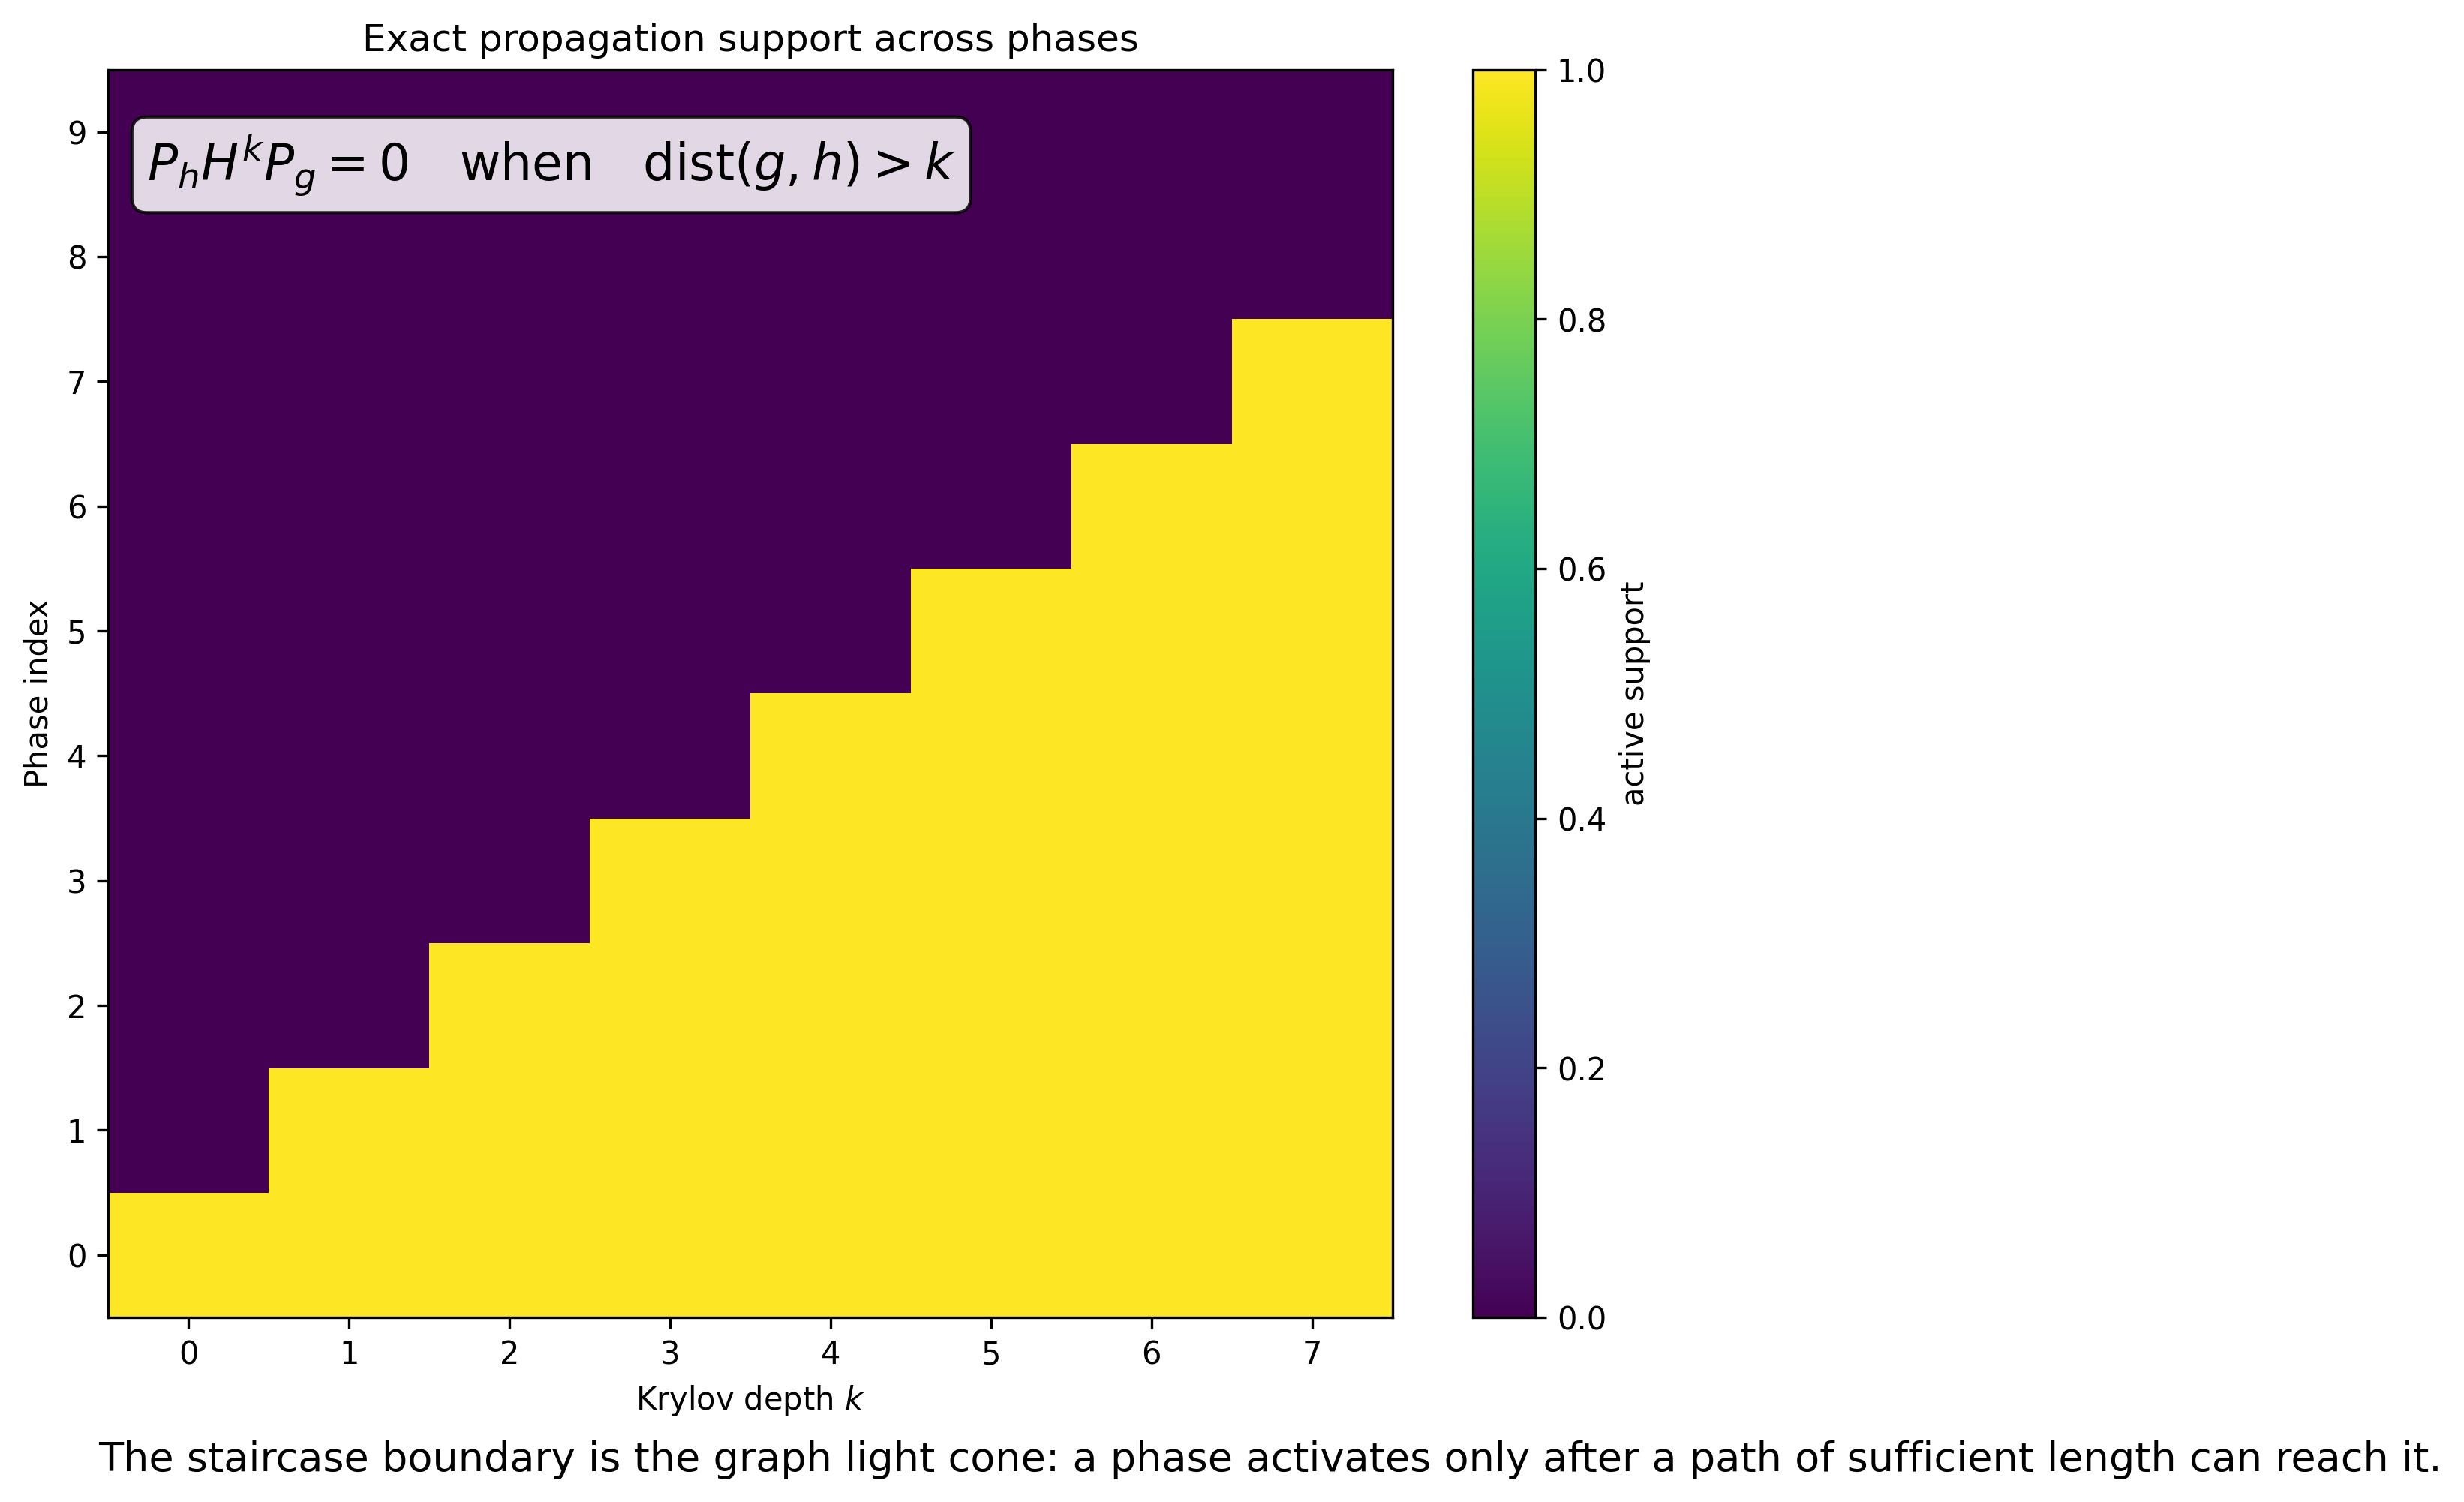
\includegraphics[width=.82\linewidth]{figure_04_polyphase_lightcone.png}
\caption{The exact polyphase light cone. The support of the Krylov iterate expands by at most one graph edge per operator application. Phases outside graph distance $k$ remain identically inactive at depth $k$ and need not be loaded.}
\label{fig:polyphase-lightcone}
\end{figure}

\begin{theorem}[Streaming-polyphase composition]
At Krylov depth \(k\), an exact matrix-free iteration may omit every phase
outside the exact light cone.  Within each active phase, arbitrary storage
refinement may be used.
\end{theorem}

\begin{proof}
The light-cone theorem removes inactive phase contributions exactly.
Partition-refinement invariance shows that the remaining active phase
operators may be streamed through any exact subpartition.
\end{proof}

This is the key composition law:
\[
\boxed{
\text{mathematical locality}
\longrightarrow
\text{active phases}
\longrightarrow
\text{active storage blocks}.
}
\]

\section{Certified approximate light cones}
\label{sec:approx-lightcone}

The exact light-cone theorem requires literal zero phase couplings.  Real LD,
annotation, and feature graphs are often only approximately sparse.  This
section replaces exact support by a computable phasewise envelope.

Let the phase projectors be $P_1,\ldots,P_q$, and let $X$ be a vector or block
vector.  Define its phase-norm profile
\[
\rho(X)_g=\lVert P_gX\rVert_F,
\]
and define the nonnegative phase-transfer matrix
\[
\mathcal B_{hg}=\lVert P_hHP_g\rVert_2.
\]
The matrix $\mathcal B$ records the strength of every one-step phase transfer
without assuming that weak couplings vanish.

\begin{theorem}[Weighted phase-transfer envelope]
\label{thm:weighted-transfer}
For every block vector $X$,
\[
\boxed{
\rho(HX)\leq \mathcal B\rho(X)
}
\]
componentwise.  Consequently, for every integer $k\geq0$,
\[
\boxed{
\rho(H^kX)\leq \mathcal B^k\rho(X).
}
\]
\end{theorem}

\begin{proof}
Using $\sum_gP_g=I$ and submultiplicativity,
\[
\begin{aligned}
\lVert P_hHX\rVert_F
&=\left\lVert\sum_gP_hHP_gX\right\rVert_F\\
&\leq\sum_g\lVert P_hHP_g\rVert_2\lVert P_gX\rVert_F\\
&=(\mathcal B\rho(X))_h.
\end{aligned}
\]
Iteration gives the power bound.
\end{proof}

Now choose a symmetric set of retained phase blocks and define
\[
H_0=\sum_{(h,g)\in\mathcal E_0}P_hHP_g.
\]
Let
\[
(\mathcal B_0)_{hg}=
\begin{cases}
\mathcal B_{hg},&(h,g)\in\mathcal E_0,\\
0,&\text{otherwise},
\end{cases}
\qquad
\mathcal R=\mathcal B-\mathcal B_0.
\]
Symmetric pair retention preserves self-adjointness of $H_0$, although the
following error theorem does not require positive semidefiniteness of $H_0$.

\begin{theorem}[Thresholded-power certificate]
\label{thm:thresholded-power}
For every $k\geq1$,
\[
\boxed{
\rho\bigl((H^k-H_0^k)X\bigr)
\leq
(\mathcal B^k-\mathcal B_0^k)\rho(X).
}
\]
In particular,
\[
\boxed{
\lVert(H^k-H_0^k)X\rVert_F
\leq
\left\lVert(\mathcal B^k-\mathcal B_0^k)\rho(X)\right\rVert_2.
}
\]
\end{theorem}

\begin{proof}
Write $E=H-H_0$.  The telescoping identity gives
\[
H^k-H_0^k
=
\sum_{j=0}^{k-1}H^{k-1-j}EH_0^j.
\]
The block-norm matrix of $E$ is $\mathcal R$.  Applying
Theorem~\ref{thm:weighted-transfer} successively to each term gives
\[
\rho\bigl((H^k-H_0^k)X\bigr)
\leq
\sum_{j=0}^{k-1}
\mathcal B^{k-1-j}\mathcal R\mathcal B_0^j\rho(X).
\]
The matrix telescoping identity
\[
\mathcal B^k-\mathcal B_0^k
=
\sum_{j=0}^{k-1}
\mathcal B^{k-1-j}(\mathcal B-\mathcal B_0)\mathcal B_0^j
\]
yields the phasewise formula.  Orthogonality of the phase projectors gives
\[
\lVert Y\rVert_F^2=\sum_h\lVert P_hY\rVert_F^2,
\]
which proves the global bound.
\end{proof}

\begin{corollary}[Certified approximate light cone]
\label{cor:approx-lightcone}
Assume $X$ is supported on a set of start phases $S$.  If phase $h$ is not
reachable from $S$ by a retained path of length at most $k$, then
\[
P_hH_0^kX=0
\]
and
\[
\boxed{
\lVert P_hH^kX\rVert_F
\leq
\bigl[(\mathcal B^k-\mathcal B_0^k)\rho(X)\bigr]_h.
}
\]
Thus an exact zero outside the retained light cone is replaced by a certified
nonzero leakage budget.
\end{corollary}

\begin{corollary}[Scalar threshold law]
For any induced matrix norm, let
\[
M=\max\{\lVert\mathcal B\rVert,\lVert\mathcal B_0\rVert\}.
\]
Then
\[
\boxed{
\lVert\mathcal B^k-\mathcal B_0^k\rVert
\leq
kM^{k-1}\lVert\mathcal R\rVert.
}
\]
Hence weak discarded coupling produces a first-order error bound proportional
to the discarded transfer norm and to the Krylov depth.
\end{corollary}

\begin{theorem}[Krylov-polynomial certificate]
\label{thm:polynomial-certificate}
Let
\[
p(t)=\sum_{j=0}^d a_jt^j.
\]
Then
\[
\boxed{
\rho\bigl((p(H)-p(H_0))X\bigr)
\leq
\sum_{j=1}^d
|a_j|(\mathcal B^j-\mathcal B_0^j)\rho(X).
}
\]
\end{theorem}

\begin{proof}
Apply Theorem~\ref{thm:thresholded-power} to every nonconstant power and use
the triangle inequality.  The constant terms cancel.
\end{proof}

The polynomial theorem covers arbitrary vectors in a finite Krylov space,
including polynomial filters and restarted combinations, rather than only the
monomial $H^kX$.

\begin{corollary}[Certified phase pruning]
If a thresholded phase graph is chosen so that
\[
\left\lVert
(\mathcal B^k-\mathcal B_0^k)\rho(X)
\right\rVert_2
\leq\tau,
\]
then replacing $H^kX$ by $H_0^kX$ incurs Frobenius error at most $\tau$.
The same statement holds for a Krylov polynomial with the certificate in
Theorem~\ref{thm:polynomial-certificate}.
\end{corollary}

This turns graph thresholding into an error-budget decision.  A phase or
interface is not discarded because it merely appears small; it is discarded
only when the weighted sum of all paths using discarded couplings remains
inside the requested tolerance.

\begin{figure}[H]
\centering
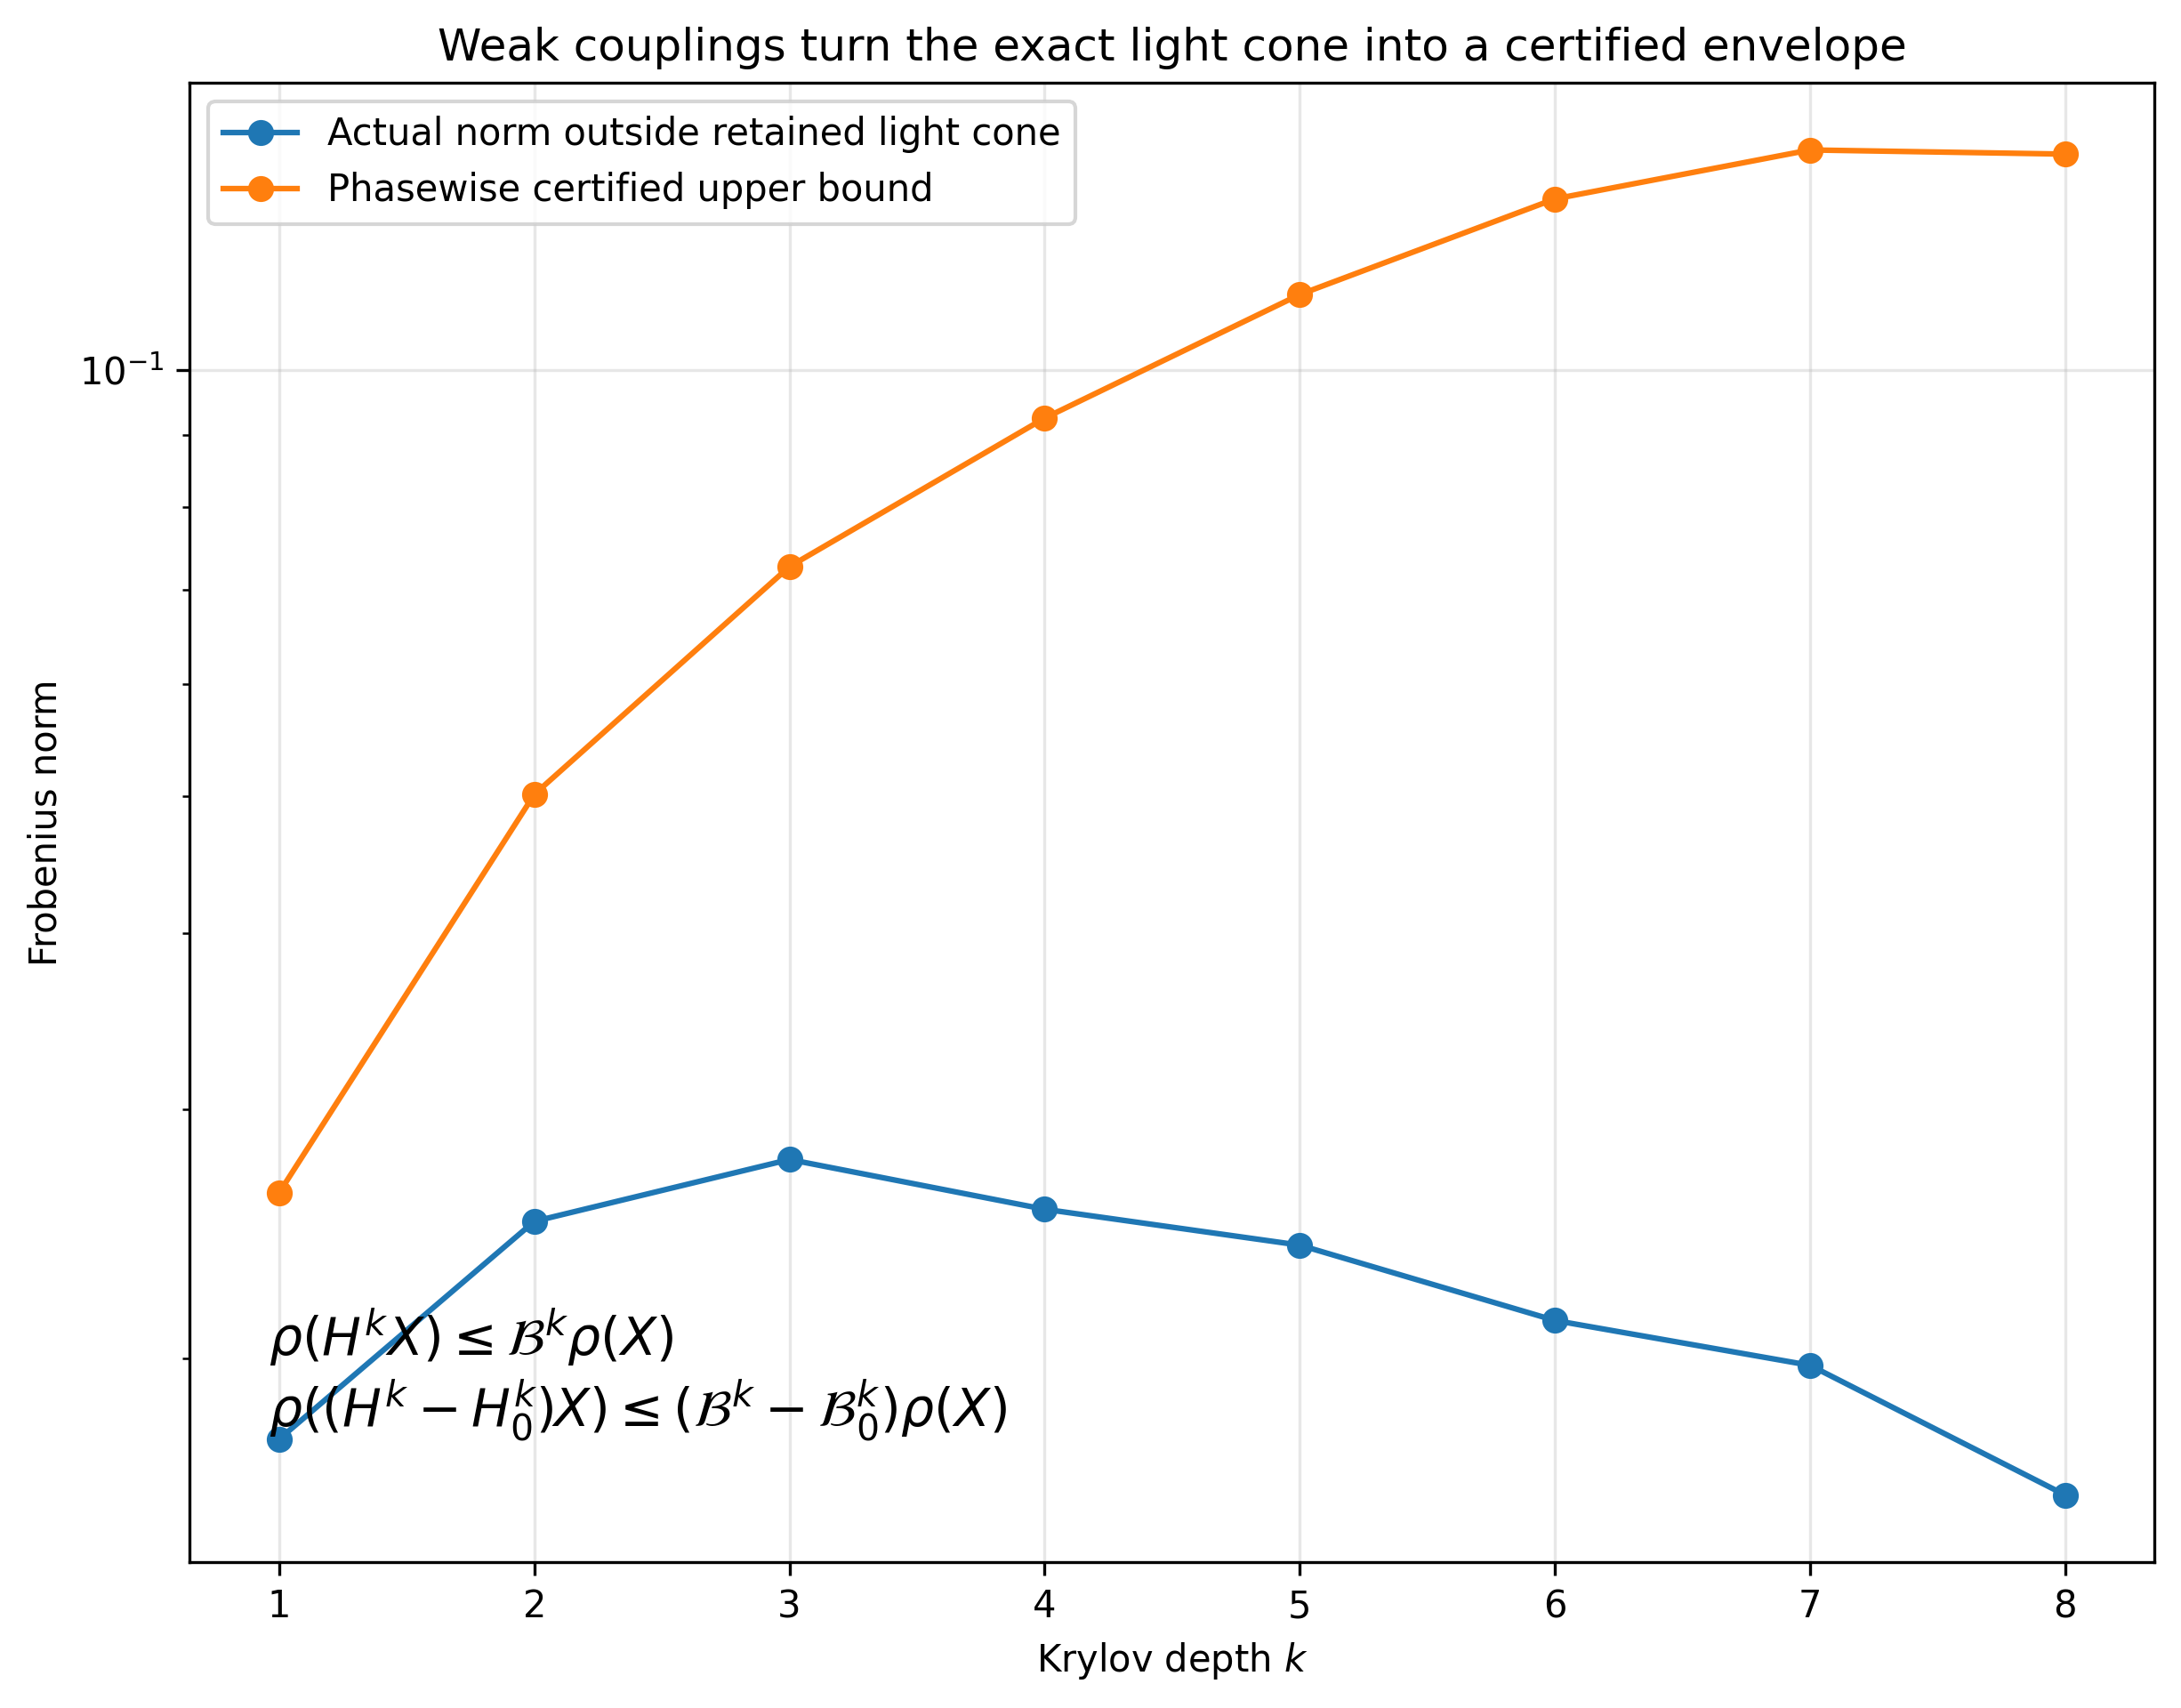
\includegraphics[width=.84\linewidth]{figure_09_approximate_lightcone_certificate.png}
\caption{Weak long-range phase couplings replace the exact zero outside the retained light cone by a nonzero but certified envelope.  In this PSD test, the phasewise transfer-matrix certificate bounds the observed leakage at every depth from one through eight.}
\label{fig:approx-lightcone-certificate}
\end{figure}

\begin{figure}[H]
\centering
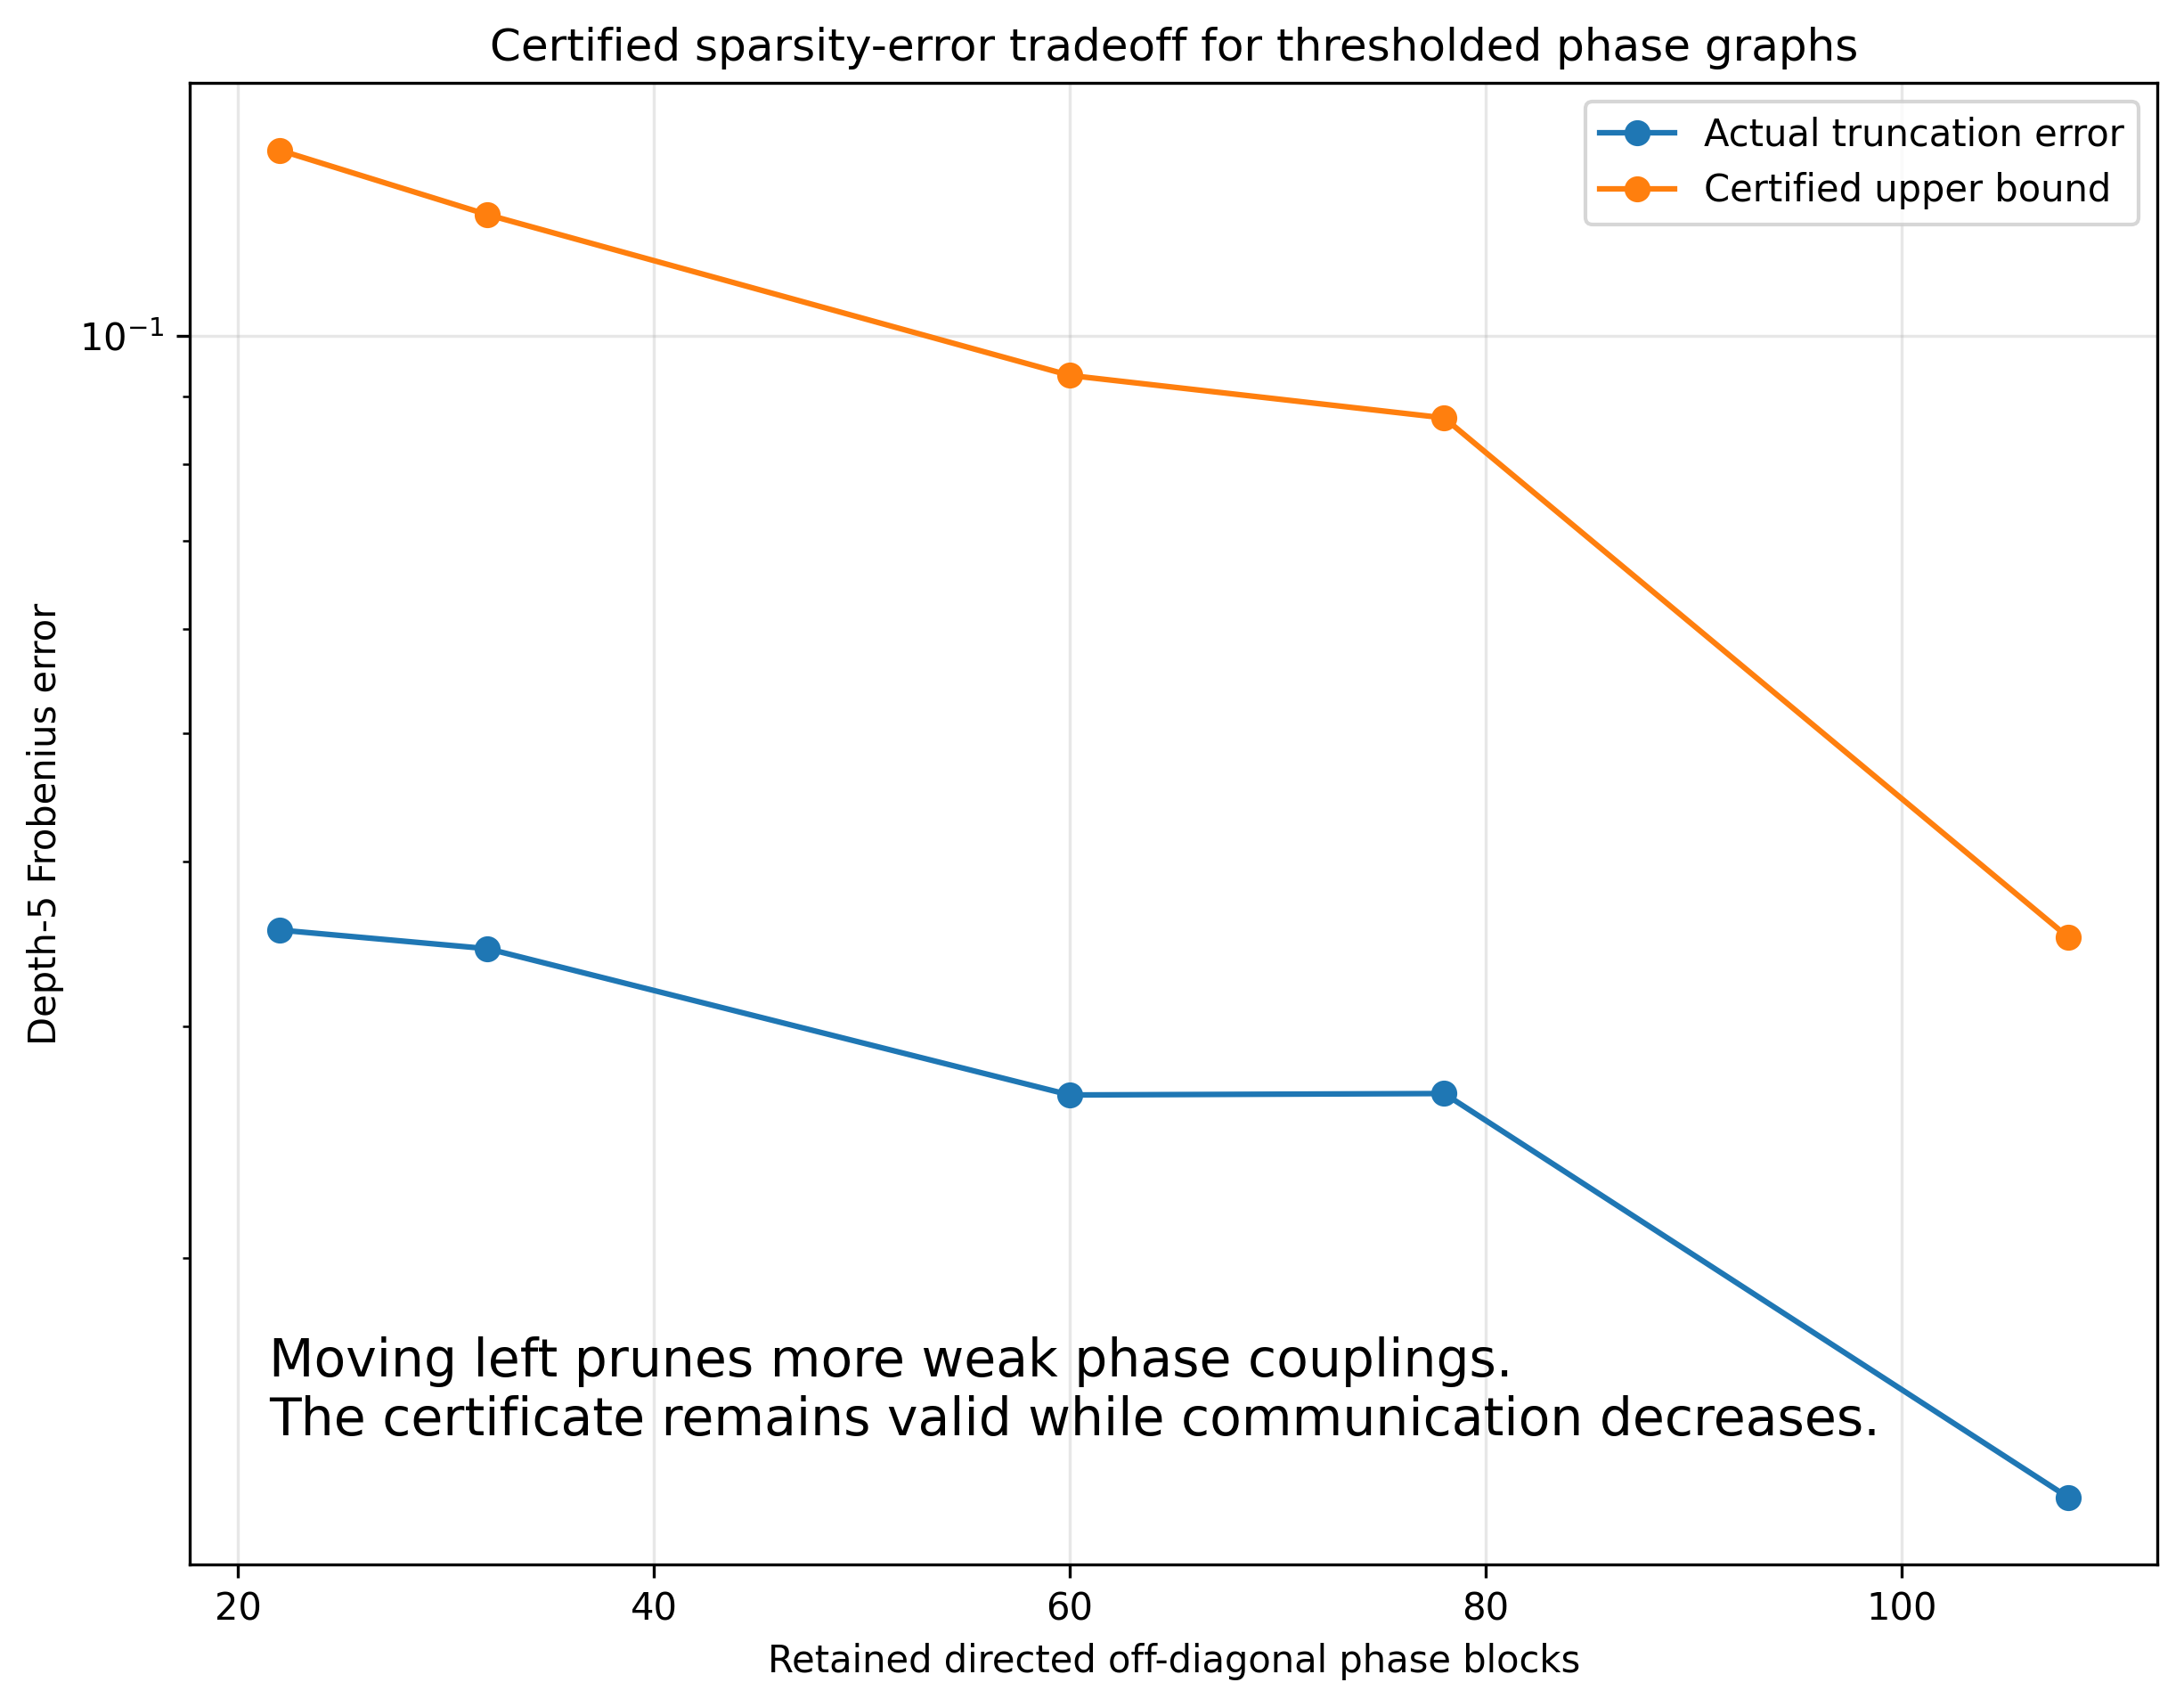
\includegraphics[width=.84\linewidth]{figure_10_threshold_tradeoff.png}
\caption{Certified phase-graph sparsification at Krylov depth five.  Retaining fewer off-diagonal phase blocks reduces communication and operator work while the transfer-matrix bound remains above the measured truncation error.  The bound is intentionally conservative because it ignores cancellation and singular-vector alignment.}
\label{fig:threshold-tradeoff}
\end{figure}

\subsection{Numerical audit}

The validation operator has twelve phases of width four.  A block-bidiagonal
factor generates a positive-definite local operator $H_0$, and weak symmetric
long-range blocks are then added to obtain $H$.  Both normalized operators
remain positive definite.  A three-column start block is supported in phase
zero.

For depths one through eight:
\begin{itemize}
\item every observed phase norm lay below $\mathcal B^k\rho(X)$;
\item every observed thresholding error lay below
$(\mathcal B^k-\mathcal B_0^k)\rho(X)$;
\item the largest total observed-error-to-certificate ratio was approximately
$0.669$.
\end{itemize}

A separate hard-threshold sweep retained between $22$ and $132$ directed
off-diagonal phase blocks.  Every measured depth-five error remained below its
certificate; the largest observed-error-to-certificate ratio was approximately
$0.376$.  Finally, a degree-four signed polynomial in $H$ satisfied the
phasewise polynomial certificate in all twelve phases, with maximum ratio
approximately $0.068$.

These computations validate the implementation and illustrate sharpness.  The
universal result is supplied by the preceding proofs, not by the finite test.


\section{Certified budget-optimal phase scheduling}
\label{sec:budget-scheduler}

The preceding section answers a validation question: given a retained phase
operator $H_0$, how large can the Krylov error be?  This section turns that
certificate into a selection rule.  The goal is to remove as much phase
communication as possible while remaining inside a prescribed error budget.

Let $\mathcal E$ denote the set of undirected off-diagonal phase pairs.  Because
$H$ is self-adjoint, $\mathcal B$ is symmetric.  For a phase pair
$e=\{h,g\}$ define the nonnegative matrix $\Delta_e$ by
\[
(\Delta_e)_{hg}=\mathcal B_{hg},\qquad
(\Delta_e)_{gh}=\mathcal B_{gh},
\]
with every other entry zero.  If $\mathcal O\subseteq\mathcal E$ is the set
of omitted pairs, define
\[
\mathcal B_{\mathcal O}
=\mathcal B-\sum_{e\in\mathcal O}\Delta_e.
\]
The diagonal is always retained.

For depth $k\ge1$ and starting phase profile $\rho_0=\rho(X)$, define the
\emph{edge risk vector}
\[
\boxed{
q_e^{(k)}
=
\sum_{j=0}^{k-1}
\mathcal B^{k-1-j}\Delta_e\mathcal B^j\rho_0
}
\]
and its scalar risk
\[
\boxed{
\beta_e^{(k)}=\lVert q_e^{(k)}\rVert_2.
}
\]
Unlike the raw block norm $\mathcal B_{hg}$, this quantity depends on the
start profile and on Krylov depth.

\begin{theorem}[Edge-additive leakage majorant]
\label{thm:edge-additive-majorant}
For every omitted set $\mathcal O\subseteq\mathcal E$,
\[
\boxed{
0\le
(\mathcal B^k-\mathcal B_{\mathcal O}^k)\rho_0
\le
\sum_{e\in\mathcal O}q_e^{(k)}
}
\]
componentwise.  Consequently,
\[
\boxed{
\lVert(H^k-H_{\mathcal O}^k)X\rVert_F
\le
\left\lVert
(\mathcal B^k-\mathcal B_{\mathcal O}^k)\rho_0
\right\rVert_2
\le
\sum_{e\in\mathcal O}\beta_e^{(k)}.
}
\]
\end{theorem}

\begin{proof}
The first inequality in the second display is
Theorem~\ref{thm:thresholded-power}.  For the transfer matrices, the exact
noncommutative telescoping identity is
\[
\mathcal B^k-\mathcal B_{\mathcal O}^k
=
\sum_{j=0}^{k-1}
\mathcal B^{k-1-j}
(\mathcal B-\mathcal B_{\mathcal O})
\mathcal B_{\mathcal O}^j.
\]
All matrices and $\rho_0$ are nonnegative, and
$0\le\mathcal B_{\mathcal O}\le\mathcal B$ entrywise.  Hence
\[
\mathcal B_{\mathcal O}^j\rho_0
\le
\mathcal B^j\rho_0.
\]
Substituting
\[
\mathcal B-\mathcal B_{\mathcal O}
=
\sum_{e\in\mathcal O}\Delta_e
\]
and distributing the sum gives the componentwise majorant.  The final scalar
bound follows from the Euclidean triangle inequality.
\end{proof}

\begin{corollary}[Polynomial edge-risk certificate]
Let
\[
p(t)=\sum_{d=0}^{D}a_dt^d.
\]
Define
\[
q_e^{(p)}
=
\sum_{d=1}^{D}|a_d|q_e^{(d)},
\qquad
\beta_e^{(p)}=\lVert q_e^{(p)}\rVert_2.
\]
Then
\[
\boxed{
\lVert(p(H)-p(H_{\mathcal O}))X\rVert_F
\le
\sum_{e\in\mathcal O}\beta_e^{(p)}.
}
\]
Thus the same scheduling machinery applies to finite Krylov combinations and
polynomial filters.
\end{corollary}

\begin{corollary}[Query-invisible phase pair]
If
\[
\Delta_e\mathcal B^j\rho_0=0
\qquad
\text{for every }0\le j<k,
\]
then
\[
\beta_e^{(k)}=0.
\]
Therefore a phase pair can be large in operator norm and still have zero
risk for a particular finite-depth query.  A magnitude-only threshold cannot
represent this distinction.
\end{corollary}

\subsection{Equal-cost optimality}

Suppose each retained phase pair has the same communication or scheduling
cost.  Under the additive certificate, a set of omitted pairs is feasible if
\[
\sum_{e\in\mathcal O}\beta_e^{(k)}\le\tau.
\]
Sort the risks as
\[
\beta_{(1)}\le\beta_{(2)}\le\cdots\le\beta_{(N)}.
\]

\begin{theorem}[Cardinality-optimal certified pruning]
\label{thm:unit-cost-optimal}
Let $r$ be the largest integer satisfying
\[
\sum_{i=1}^{r}\beta_{(i)}\le\tau.
\]
Then omitting the $r$ least-risk phase pairs is feasible, and no feasible
omitted set can contain more than $r$ pairs under the scalar additive
certificate.
\end{theorem}

\begin{proof}
Among all subsets of cardinality $r+1$, the smallest possible sum of risks is
\[
\sum_{i=1}^{r+1}\beta_{(i)}.
\]
By maximality of $r$, that sum exceeds $\tau$.  Hence no set of $r+1$ omitted
pairs is feasible.  The prefix of length $r$ is feasible by construction.
\end{proof}

This is a genuine optimization theorem, not a heuristic threshold rule.  The
optimization target is the additive certificate itself; the tighter exact
transfer envelope can leave additional slack.

\subsection{Exact-envelope refinement}

After the cardinality-optimal additive schedule is found, recomputing
\[
\left\lVert
(\mathcal B^k-\mathcal B_{\mathcal O}^k)\rho_0
\right\rVert_2
\]
may reveal unused budget.  Additional pairs can then be removed one at a time,
provided the exact transfer envelope remains below $\tau$.

\begin{proposition}[Certified refinement]
Any sequence of additional omissions accepted only when
\[
\left\lVert
(\mathcal B^k-\mathcal B_{\mathcal O}^k)\rho_0
\right\rVert_2\le\tau
\]
remains a valid $\tau$-certificate for the original operator error.
\end{proposition}

The refinement rule used in the reference implementation chooses, among all
currently feasible next omissions, the pair that produces the smallest
increase in the exact transfer envelope.  It is certified but is not claimed
globally optimal.

\subsection{Unequal communication costs}

Let $c_e\ge0$ denote the communication or storage cost saved by omitting pair
$e$.  Under the scalar additive certificate, the exact discrete selection
problem is
\[
\boxed{
\max_{x_e\in\{0,1\}}
\sum_e c_ex_e
\quad\text{subject to}\quad
\sum_e\beta_e^{(k)}x_e\le\tau.
}
\]
This is the $0$--$1$ knapsack problem.  Hence unequal-cost scheduling is
combinatorial in general.  The implementation supplies a safe
cost-to-risk greedy heuristic; its output remains certified because it never
exceeds the additive risk budget.  A fractional-knapsack relaxation supplies
an upper bound on the maximum possible saved cost.

\begin{figure}[H]
\centering
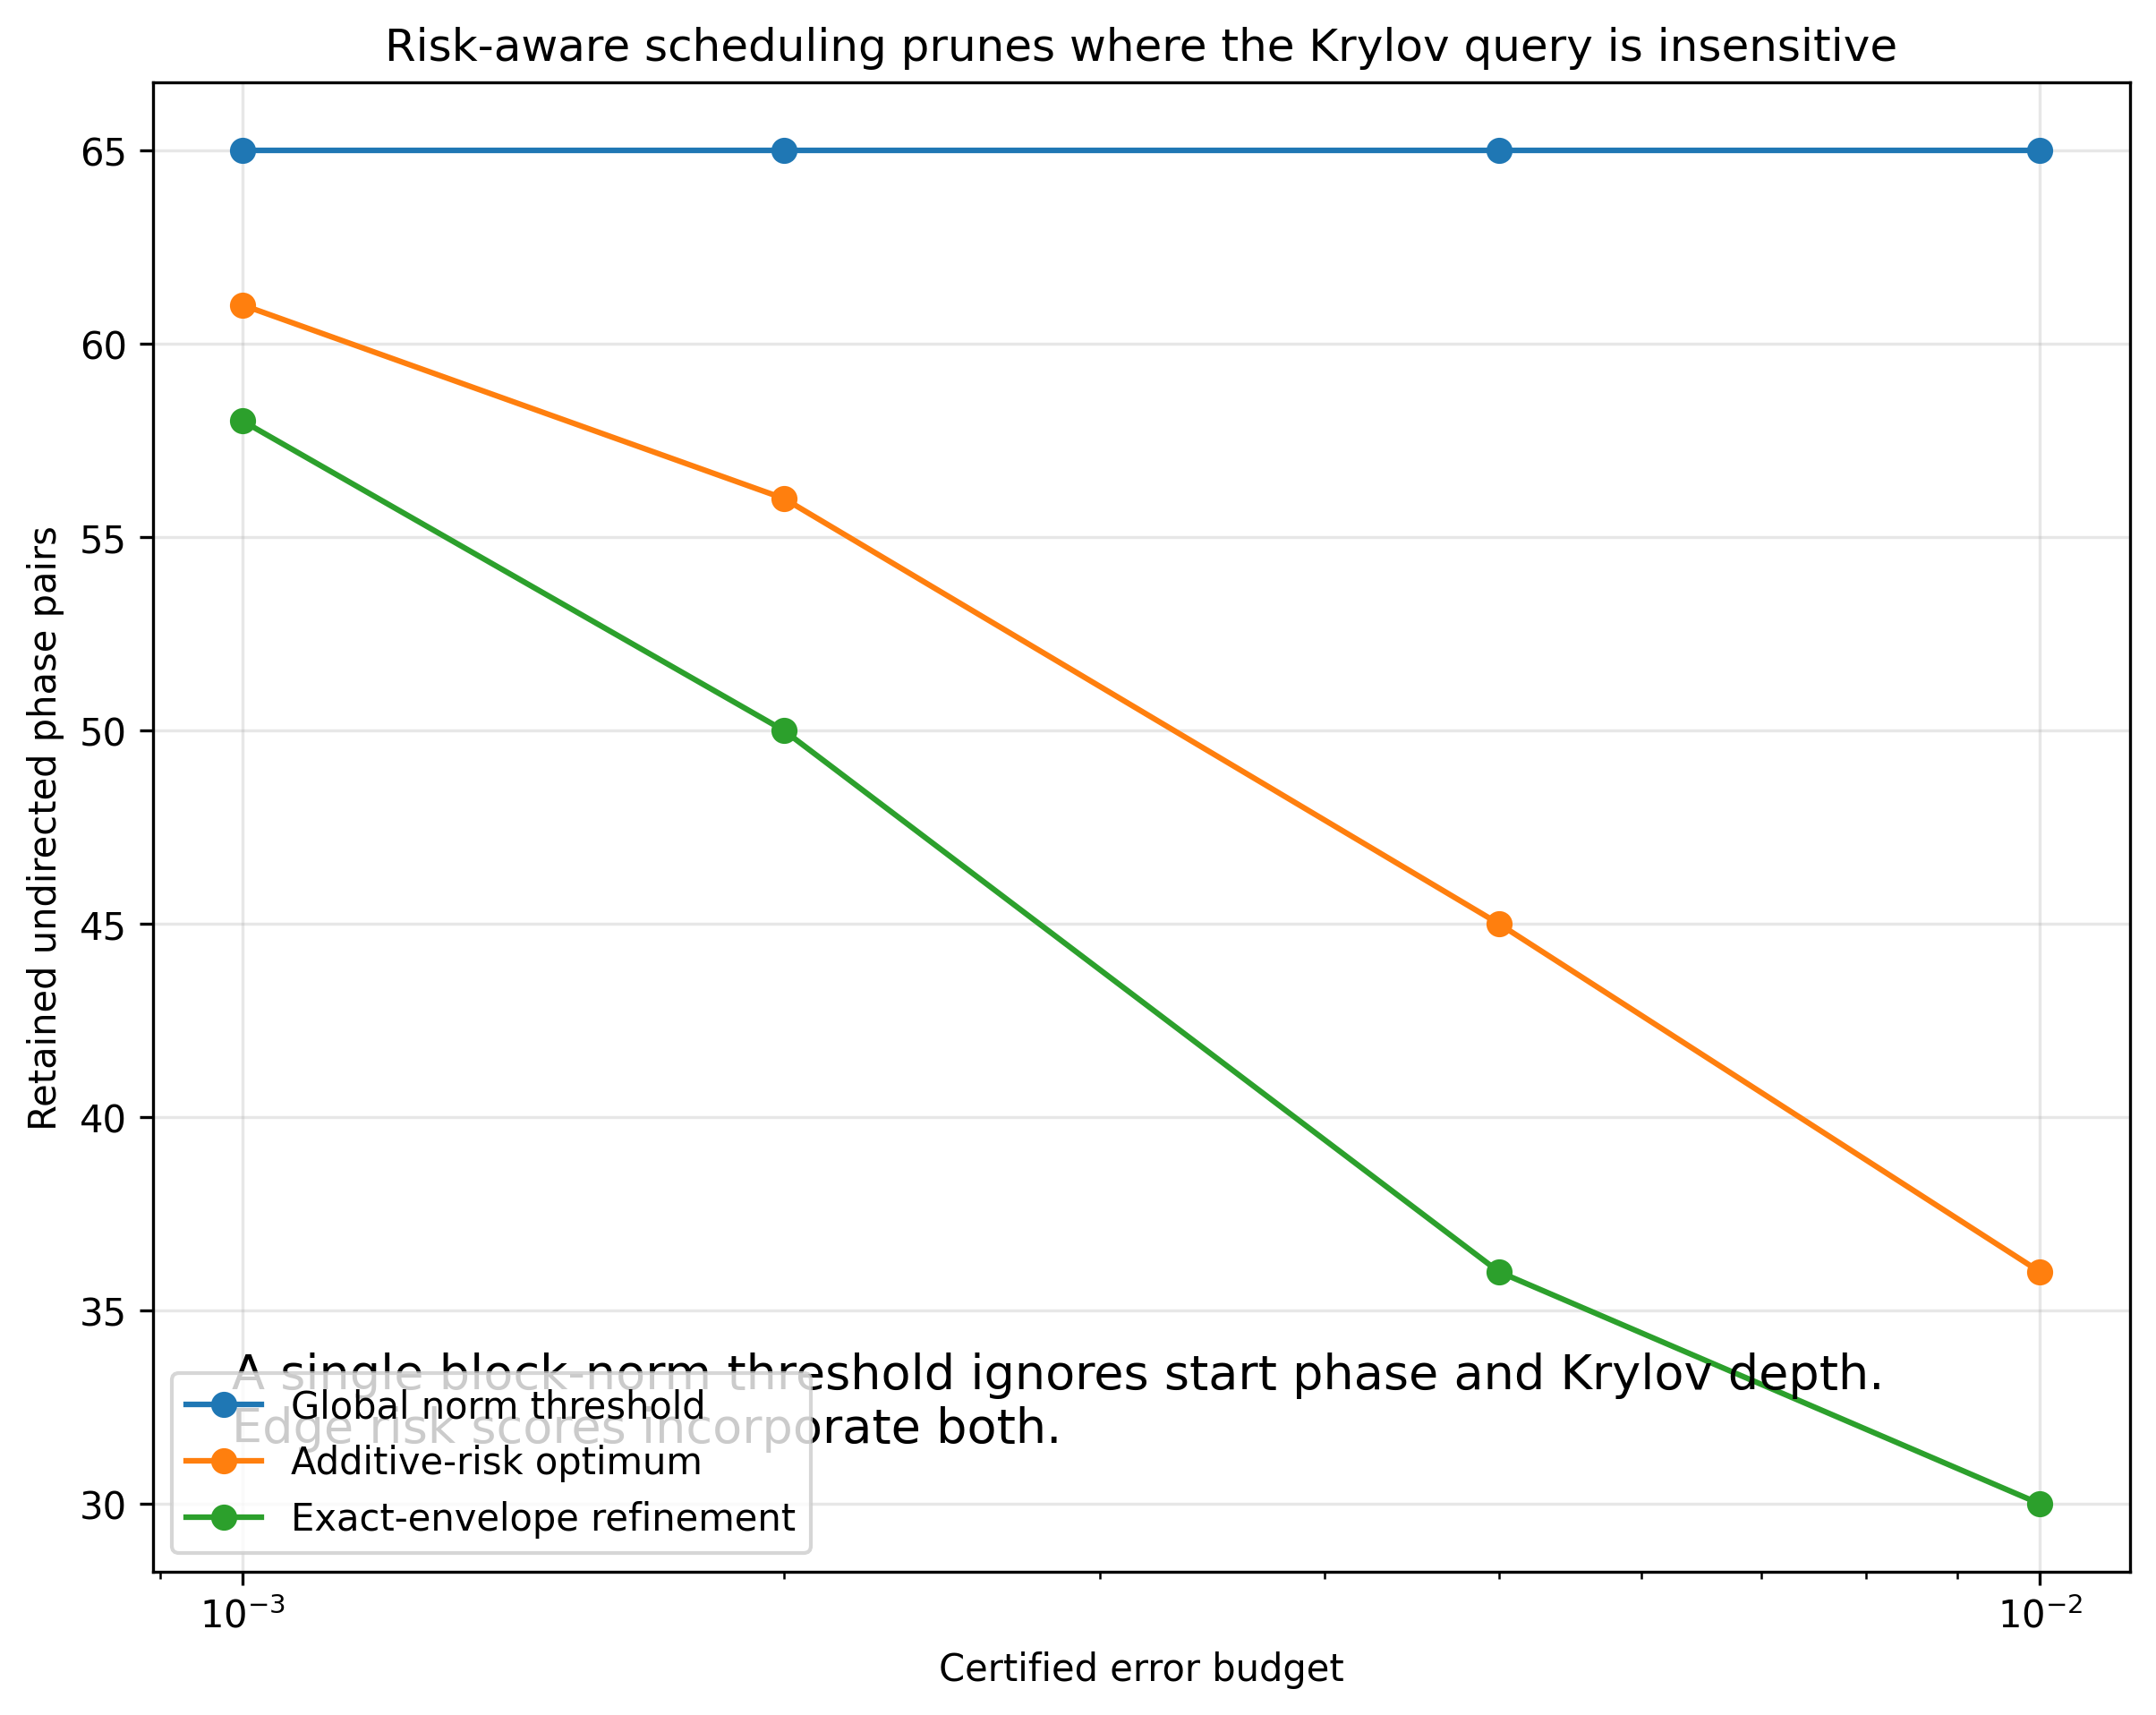
\includegraphics[width=.84\linewidth]{figure_11_budget_scheduler_comparison.png}
\caption{Depth-five pruning under a fixed certified error budget.  A global block-norm threshold is nearly unable to prune this example without crossing the requested tolerance, whereas query-aware edge risks remove many phase pairs.  The exact-envelope refinement safely uses slack left by the additive majorant.}
\label{fig:budget-scheduler-comparison}
\end{figure}

\begin{figure}[H]
\centering
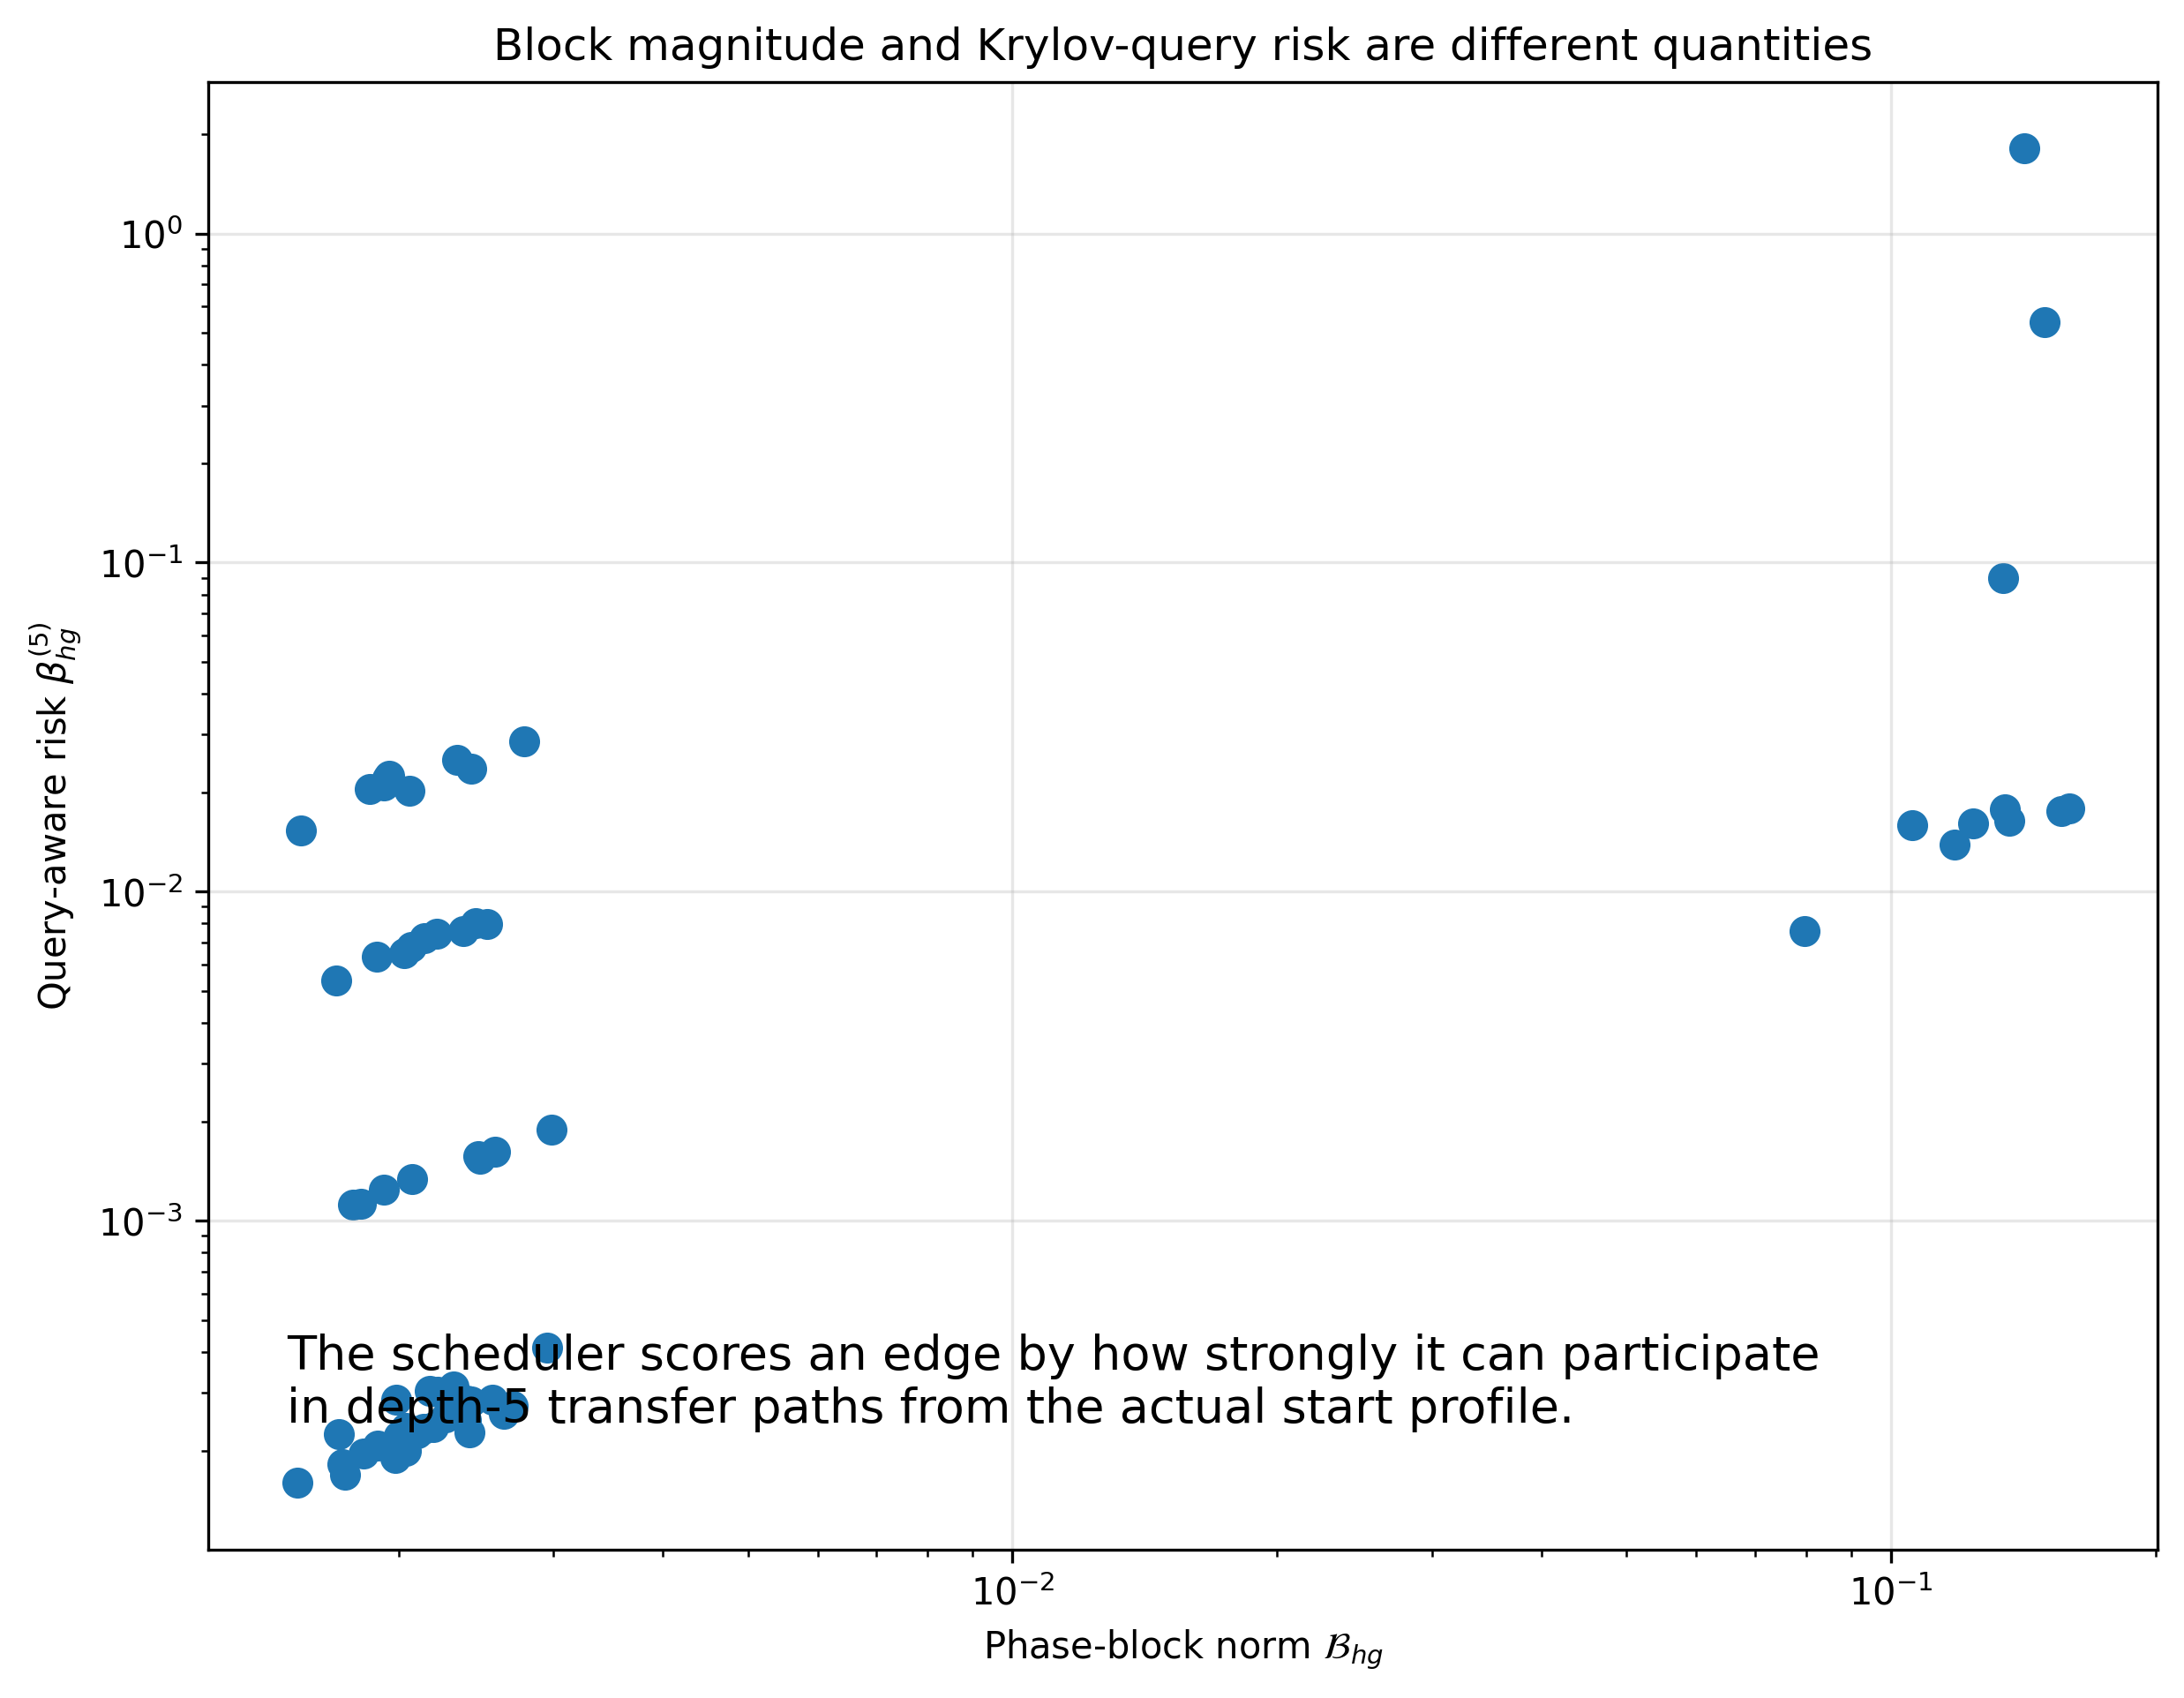
\includegraphics[width=.82\linewidth]{figure_13_edge_risk_vs_block_norm.png}
\caption{Raw phase-block magnitude and finite-depth query risk are different quantities.  The edge score $\beta_{hg}^{(5)}$ incorporates the start profile and every depth-five transfer path through the phase graph; the block norm $\mathcal B_{hg}$ does not.}
\label{fig:edge-risk-vs-norm}
\end{figure}

\subsection{Numerical audit}

The twelve-phase operator from Section~\ref{sec:approx-lightcone} was reused at
Krylov depth five.  There are $66$ undirected off-diagonal phase pairs.
For error budgets $10^{-3}$, $2\times10^{-3}$, $5\times10^{-3}$, and
$10^{-2}$, the additive-optimal scheduler retained respectively
$61$, $56$, $45$, and $36$ pairs.  Exact-envelope refinement reduced those
counts further to
$58$, $50$, $36$, and $30$ pairs while remaining inside budget.

In the same test, the best single global threshold on the raw block norm
retained $65$ pairs at every one of those four budgets.  The difference is
structural: the global threshold is blind to start phase and Krylov depth.

A separate six-phase problem contains $15$ candidate phase pairs, so all
$2^{15}=32768$ subsets can be enumerated.  At four distinct budgets, the
sorted-risk scheduler matched the brute-force cardinality optimum under the
additive certificate in every case.  The exact-envelope greedy refinement also
matched the brute-force exact-envelope optimum in cardinality for all four
budgets in this finite audit.  The latter agreement is empirical and is not
promoted to a theorem.

For an unequal-cost eight-phase test, costs were proportional to the bytes in
symmetric dense phase blocks.  The cost-to-risk heuristic saved $5408$ bytes
out of a $9472$-byte communication proxy while using additive risk $0.011632$
under budget $0.012$.  The fractional relaxation upper bound was $5647.8$
bytes, placing the greedy schedule within about $4.25\%$ of that relaxation
bound on this instance.

\section{Asynchronous double-buffer execution model}
\label{sec:double-buffer}

The mathematical streaming identities do not require transfers and GEMMs to be
serial.  Consider $B$ storage blocks.  Let $t_b$ be the transfer time for block
$b$ and $c_b$ its device compute time.

\begin{proposition}[Ideal two-buffer pipeline]
In a model with perfect asynchronous overlap, transfer of block $b+1$ may run
while block $b$ is being processed.  The serial one-buffer time is
\[
T_{\rm serial}=\sum_{b=1}^{B}(t_b+c_b),
\]
whereas the two-buffer pipeline time is
\[
\boxed{
T_{\rm pipe}
=
t_1
+
\sum_{b=1}^{B-1}\max\{c_b,t_{b+1}\}
+
c_B.
}
\]
For uniform times $t_b=t$ and $c_b=c$,
\[
T_{\rm pipe}=t+c+(B-1)\max\{t,c\}.
\]
\end{proposition}

\begin{proof}
After the first block arrives, every interior pipeline stage finishes only when
both the current computation and the next transfer have completed.  Their
joint stage duration is therefore the maximum of those two times.  The initial
transfer and final compute cannot be hidden and form the two boundary terms.
\end{proof}

If one resident block uses $M_{\rm block}$ bytes and all other fixed working
state uses $M_{\rm fixed}$ bytes, the corresponding memory models are
\[
M_{\rm single}=M_{\rm fixed}+M_{\rm block},
\qquad
\boxed{
M_{\rm double}=M_{\rm fixed}+2M_{\rm block}.
}
\]
The proposition is a scheduling model, not a hardware timing claim.  PCIe or
NVLink contention, kernel launch overhead, synchronization, page pinning, and
library workspaces can reduce realized overlap.

\begin{figure}[H]
\centering
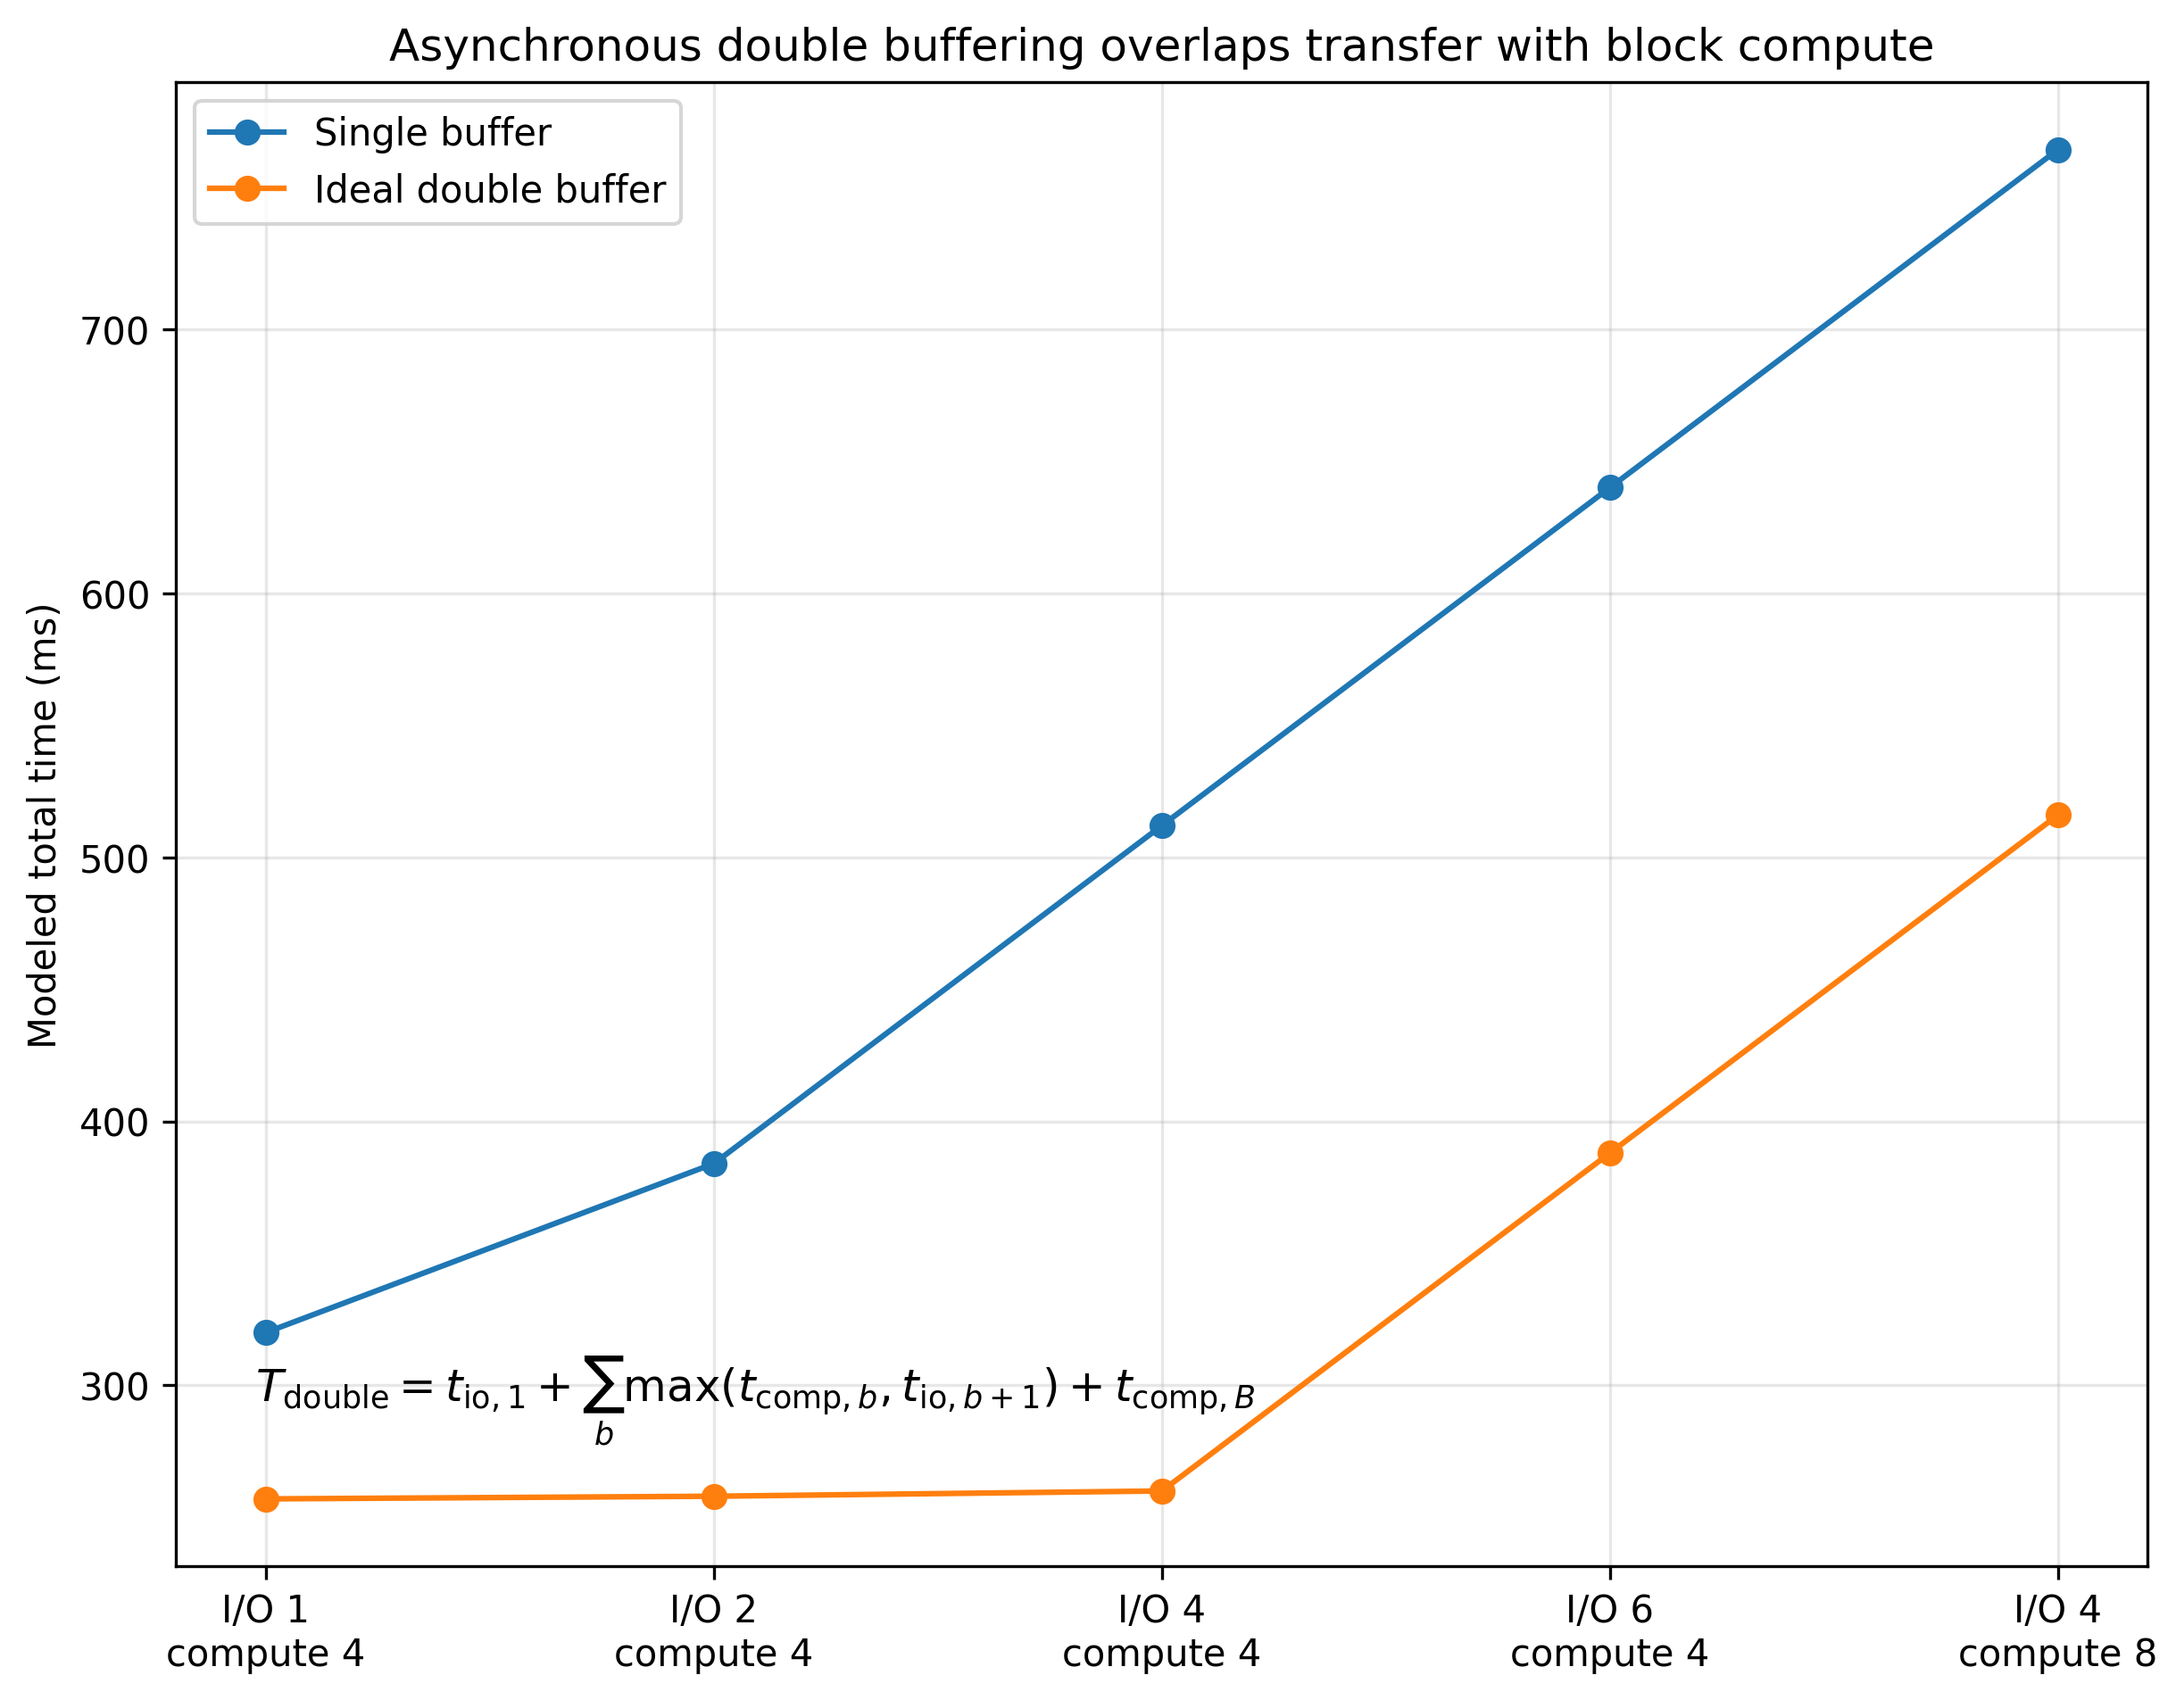
\includegraphics[width=.82\linewidth]{figure_12_double_buffer_model.png}
\caption{Idealized effect of asynchronous double buffering over $64$ streamed blocks.  The largest modeled speedup occurs when transfer and computation times are comparable, because neither resource is left idle for most of the pipeline.  The additional cost is one extra resident block buffer.}
\label{fig:double-buffer-model}
\end{figure}

\section{Phase-local rank}

Let \(R\) be a newly generated Krylov residual and
\[
R_h=P_hR.
\]

\begin{theorem}[Minimal exact phase width]
Let
\[
r_h=\operatorname{rank}(R_h).
\]
Every phase-supported basis spanning \(\operatorname{range}(R_h)\) has at
least \(r_h\) vectors, and a rank-revealing QR or compact SVD attains exactly
\(r_h\).
\end{theorem}

This justifies nonuniform Krylov block widths by phase.


\begin{figure}[H]
\centering
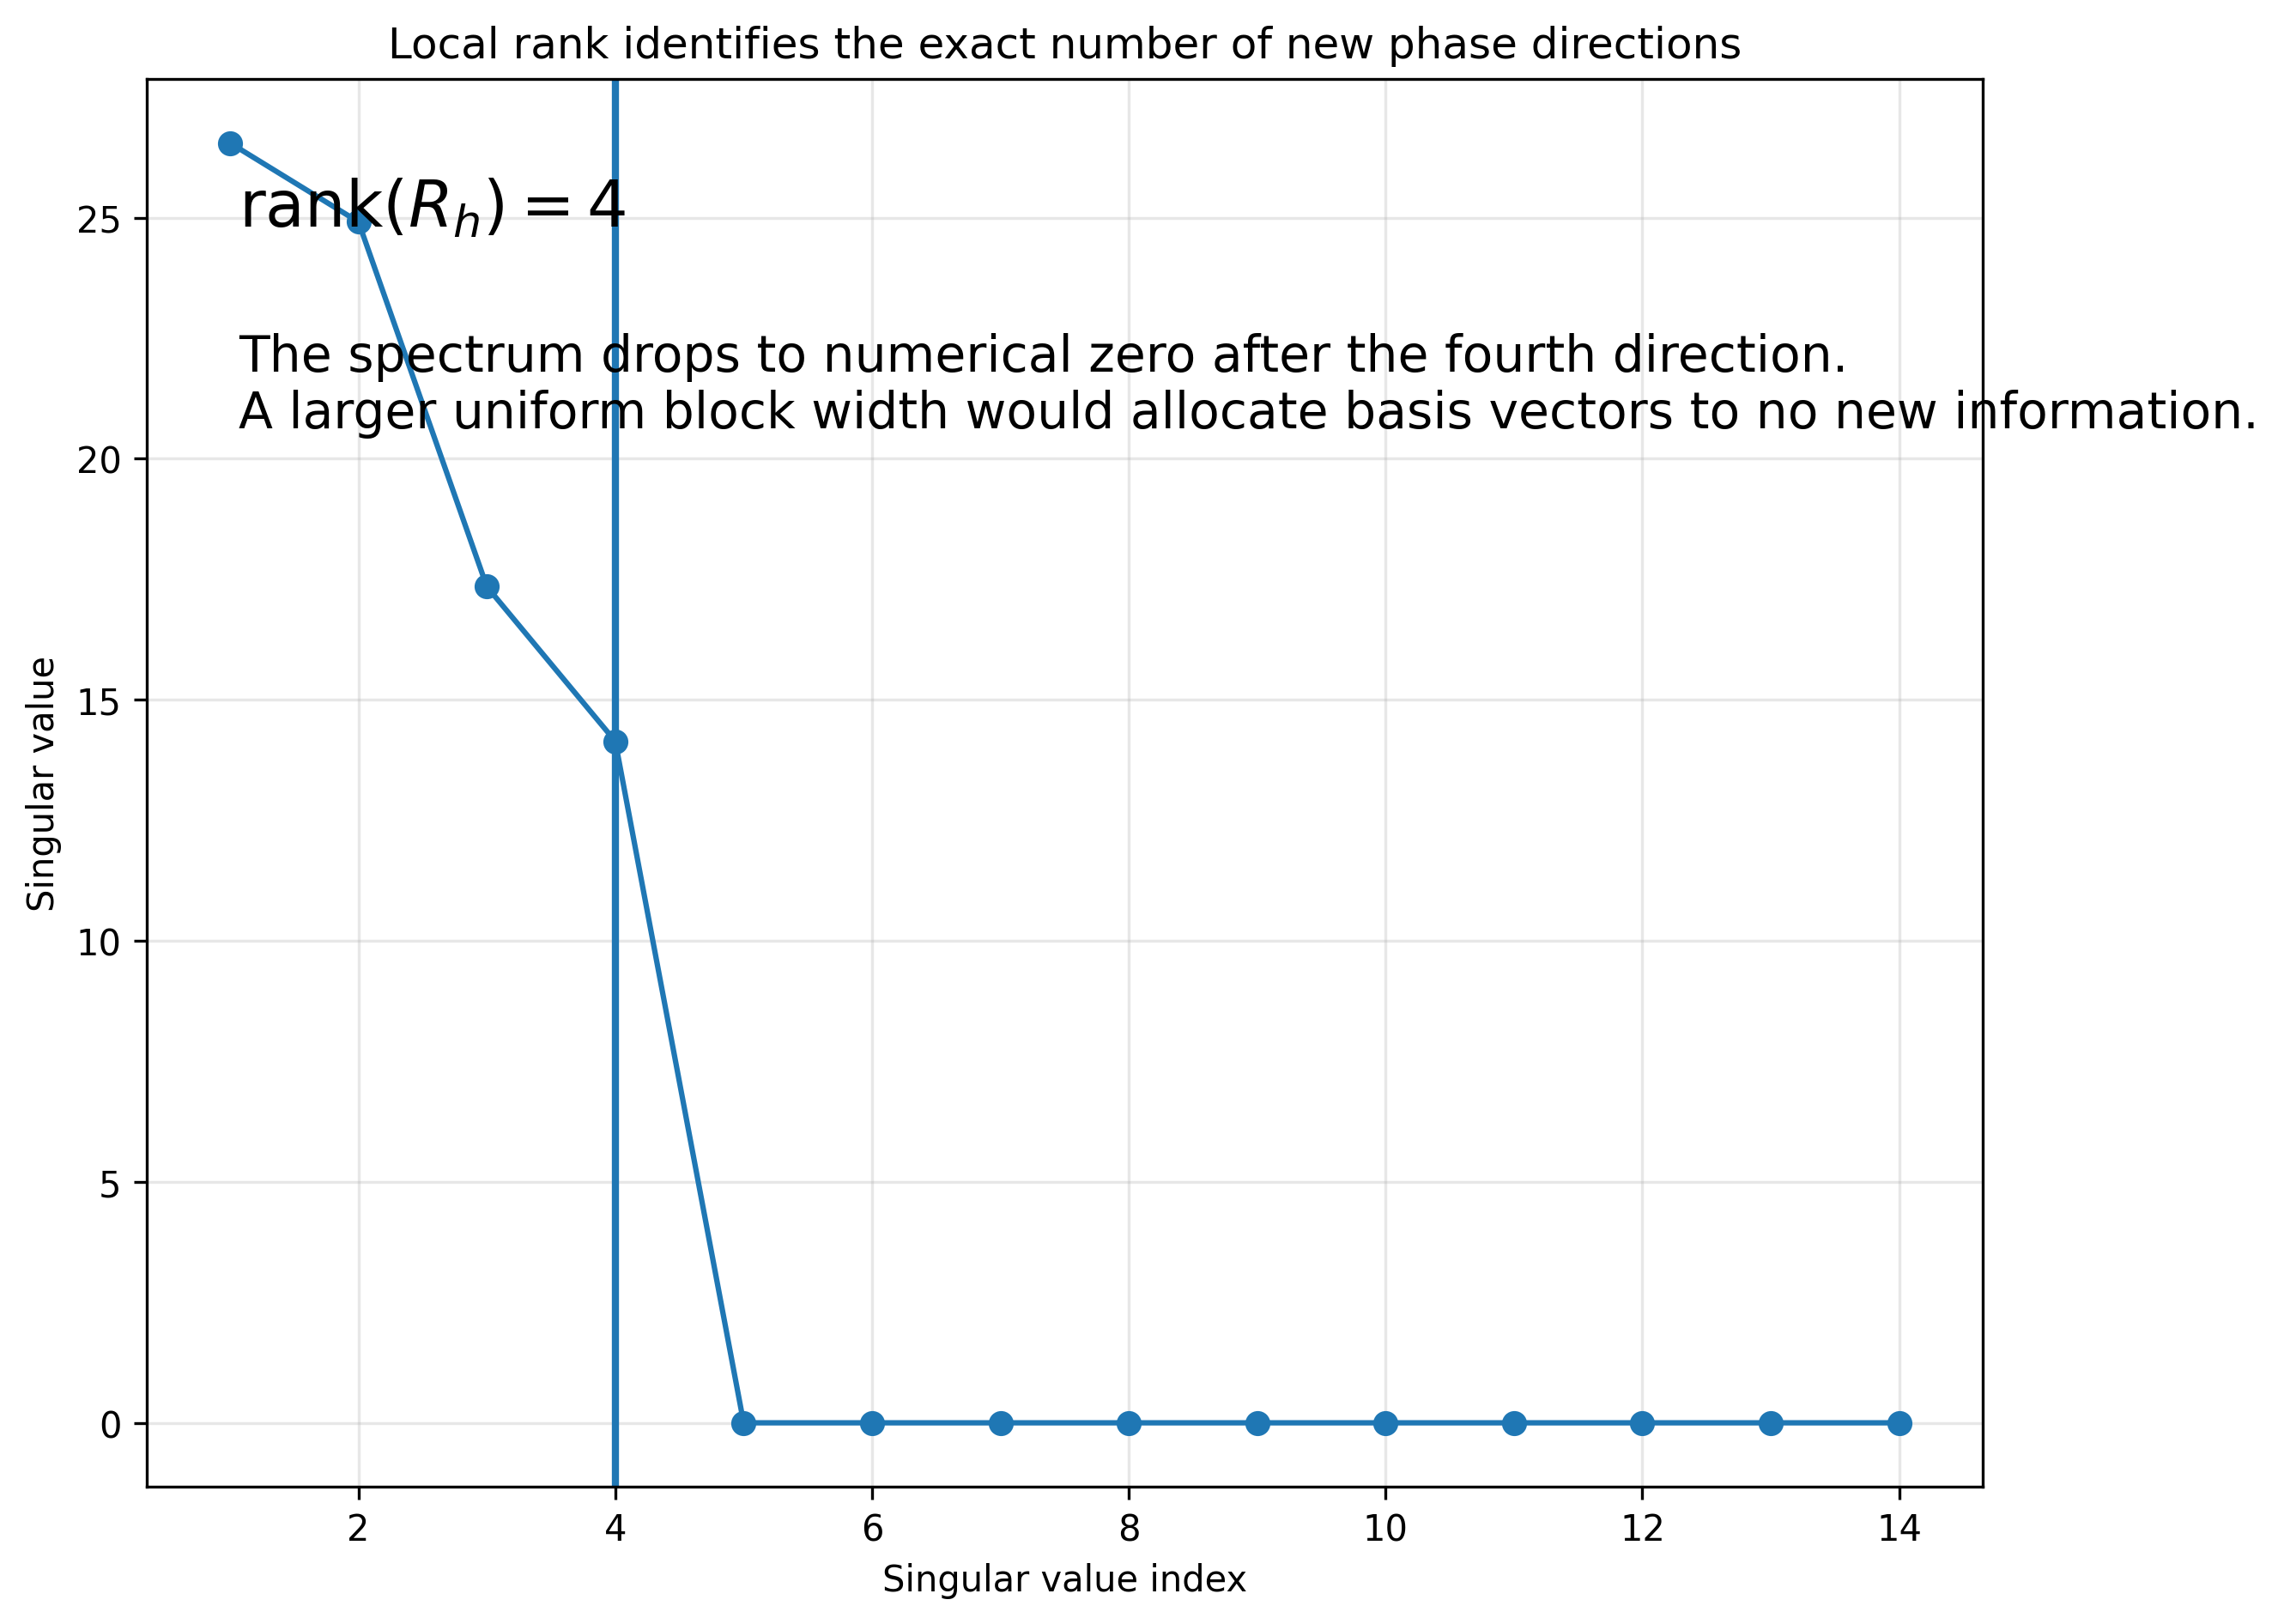
\includegraphics[width=.82\linewidth]{figure_05_phase_local_rank.png}
\caption{Phase-local rank as a dimension law. The singular values of a phase residual reveal how many genuinely new directions that phase contributes. A rank-revealing factorization keeps exactly those directions instead of allocating a uniform global width.}
\label{fig:phase-local-rank}
\end{figure}

\section{Low-rank interface messages}

If an inter-phase coupling has exact factorization
\[
P_hHP_g
=
U_{hg}V_{hg}^\top
\]
of rank \(r_{hg}\), then
\[
\boxed{
P_hHP_gx
=
U_{hg}(V_{hg}^\top x).
}
\]

This representation reduces storage and communication.  It does not
automatically reduce wall-clock time unless the factors are applied through
batched or fused kernels; a Python reference implementation can lose to
dense BLAS despite lower arithmetic and storage.

\section{Exact QR-core updates}

Suppose
\[
A=QR,
\qquad
Q^\top Q=I,
\]
and append a new block \(U\).  Set
\[
C=Q^\top U,
\qquad
F=U-QC,
\qquad
F=Q_\perp R_\perp.
\]

\begin{theorem}[Exact QR-core update]
\[
[A,U]
=
[Q,Q_\perp]
\begin{pmatrix}
R&C\\
0&R_\perp
\end{pmatrix}.
\]
Therefore the nonzero eigenvalues of
\([A,U][A,U]^\top\) are exactly the eigenvalues of the small core Gram.
\end{theorem}

This is useful for overlapping genomic windows and small incremental variant
updates.


\begin{figure}[H]
\centering
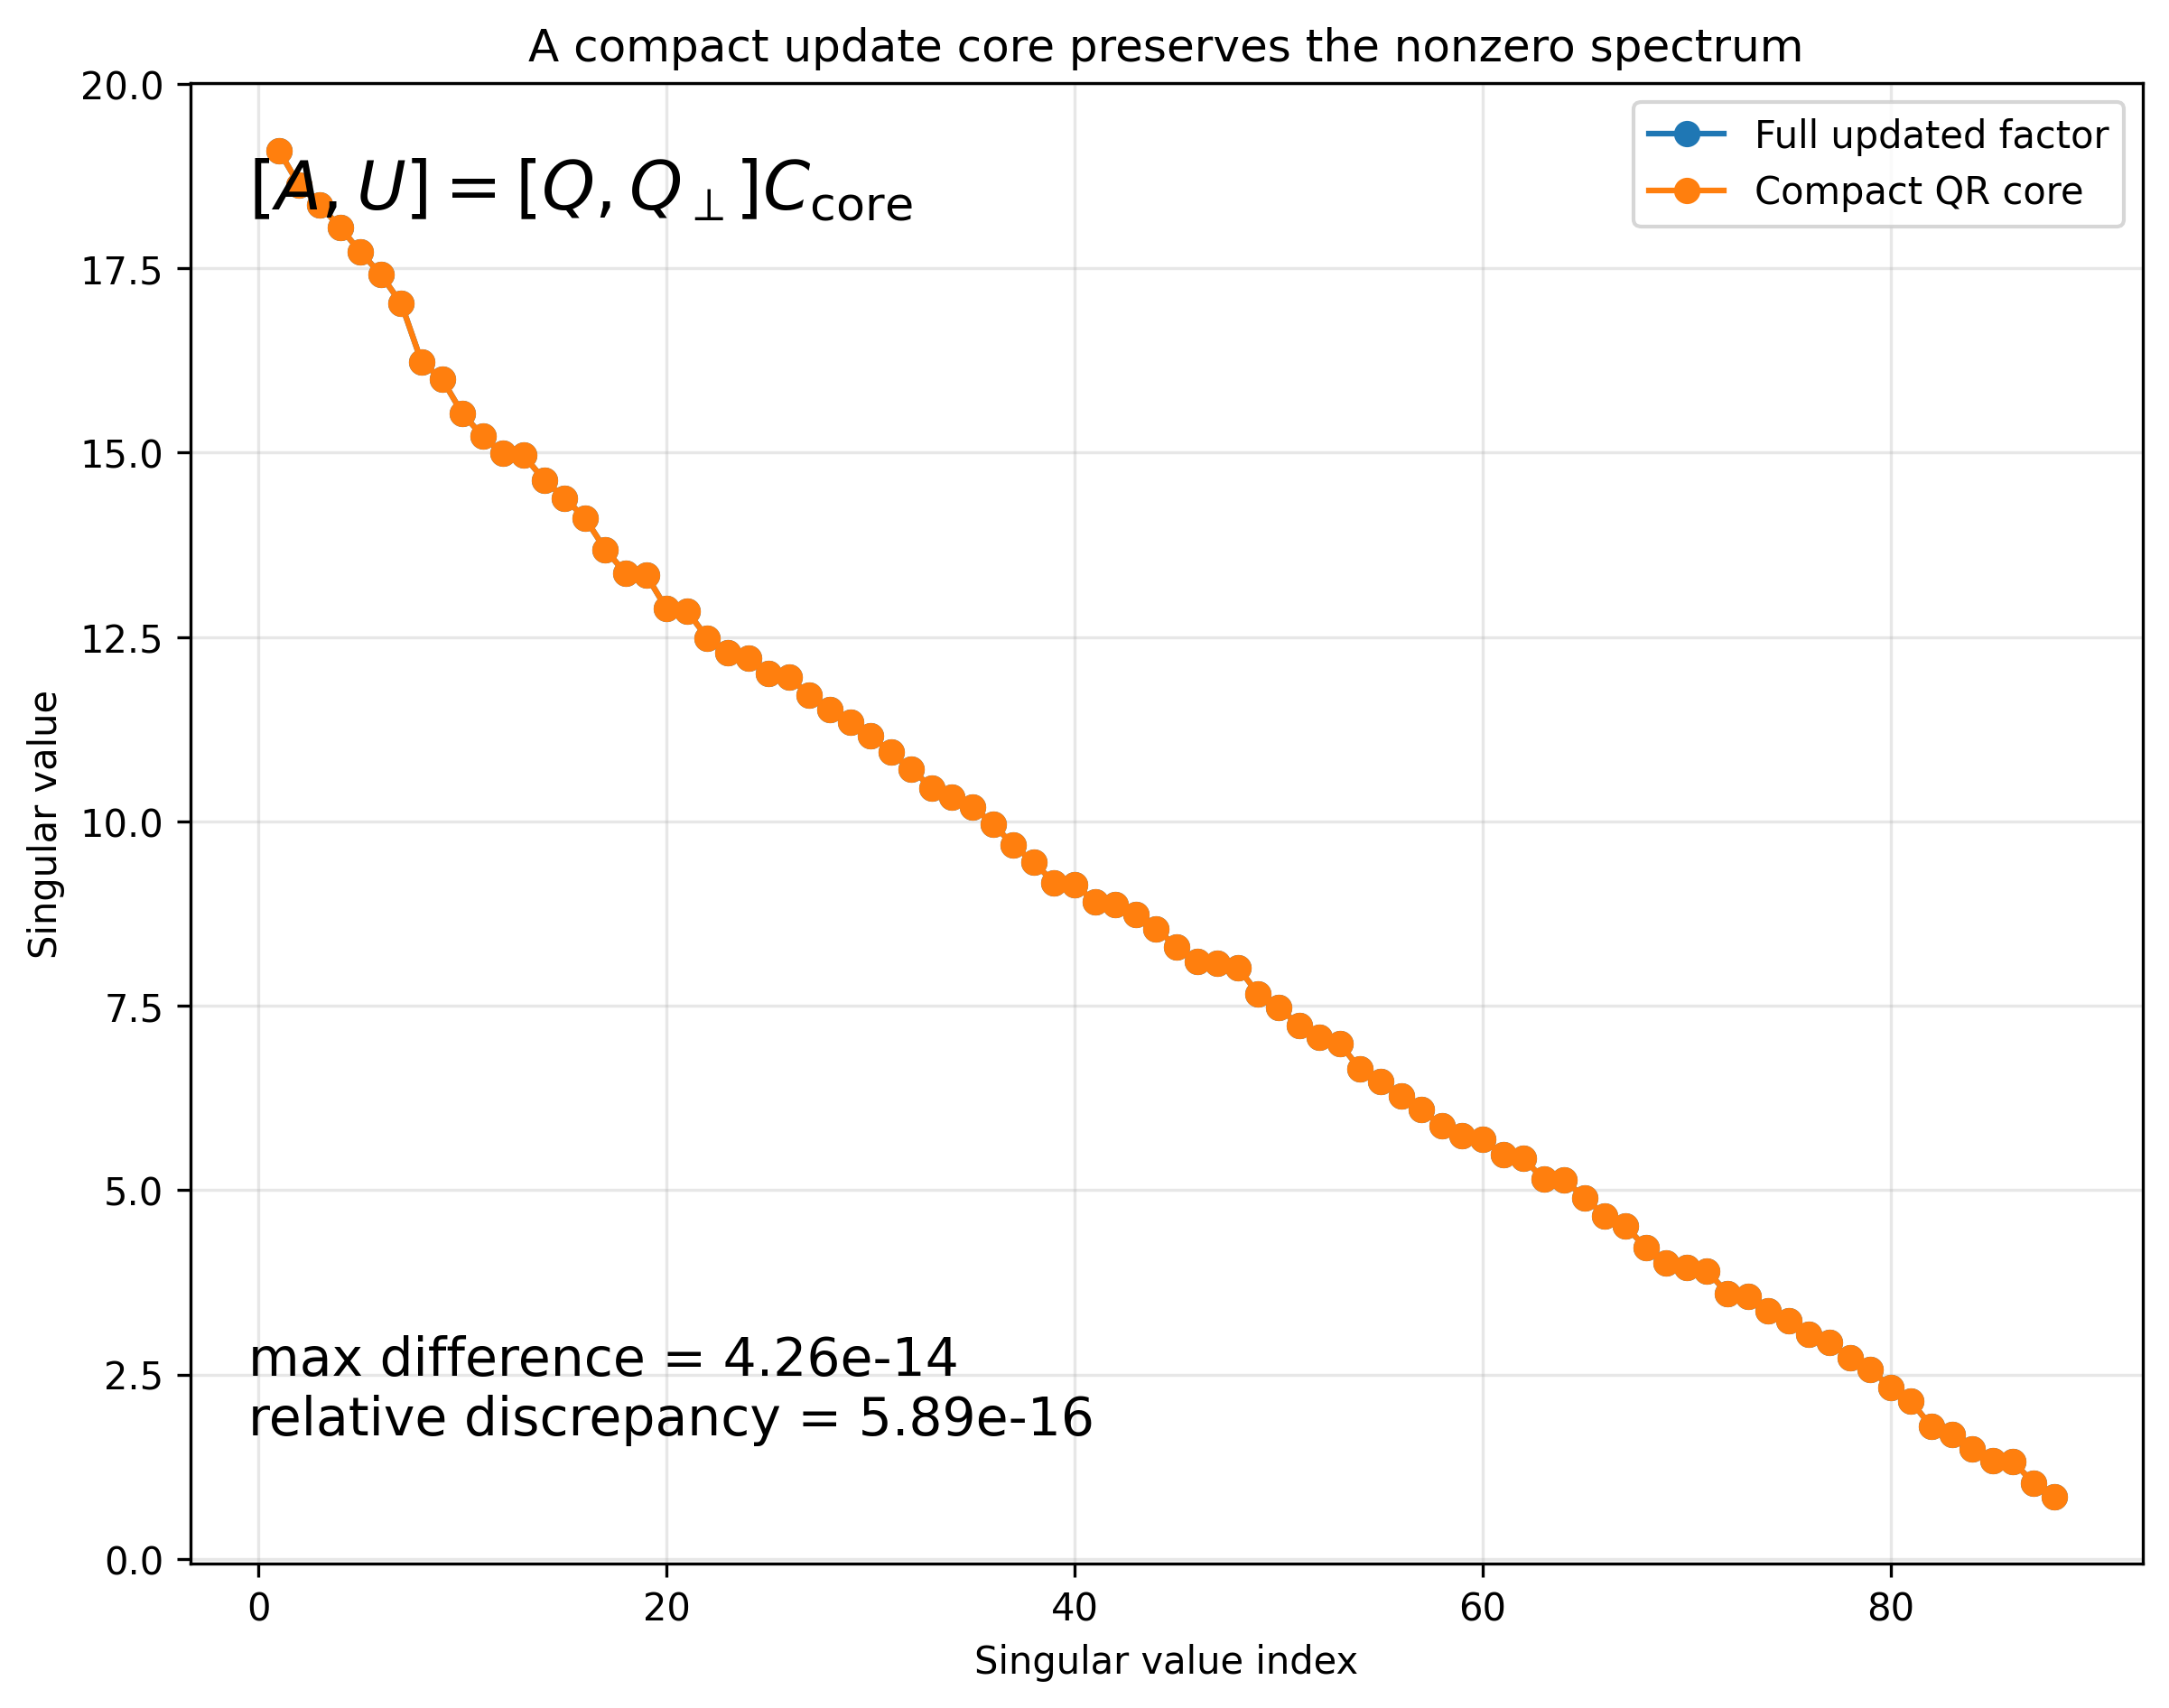
\includegraphics[width=.84\linewidth]{figure_06_qr_core_equivalence.png}
\caption{QR-core spectral equivalence. The singular values of the full updated factor and the compact update core lie on top of one another. This permits exact reuse across overlapping windows or appended variant blocks.}
\label{fig:qr-core-equivalence}
\end{figure}

\section{Range-core spectral compression}

Suppose an orthonormal basis \(Q_r\) captures the factor range:
\[
\operatorname{range}(A)\subseteq\operatorname{range}(Q_r).
\]
Then
\[
A=Q_rB,
\qquad
B=Q_r^\top A.
\]

\begin{theorem}[Exact range core]
The nonzero eigenvalues of
\[
K=AA^\top
\]
are exactly the eigenvalues of
\[
BB^\top.
\]
\end{theorem}

Thus the computational pipeline can terminate its data-streaming stage after
the range is captured:
\[
\boxed{
\text{streamed data}
\to
\text{small spectral core}
\to
\text{tail evaluation}.
}
\]

\section{From phase pruning to certified SKAT tails}

The previous sections certify the effect of phase pruning on Krylov
propagation.  A SKAT-like test ultimately depends on the spectrum itself, so
one more bridge is needed:
\[
\text{phase pruning}
\longrightarrow
\text{operator error}
\longrightarrow
\text{spectral error}
\longrightarrow
\text{tail-probability error}.
\]

\subsection{Block-norm operator domination}

Let
\[
E=H-H_0
\]
be the self-adjoint error introduced by phase pruning.  Using the same
orthogonal phase projectors \(P_h\), define
\[
\mathcal C_{hg}
=
\|P_hEP_g\|_2.
\]

\begin{theorem}[Block-norm operator certificate]
\[
\boxed{
\|E\|_2
\le
\|\mathcal C\|_2.
}
\]
\end{theorem}

\begin{proof}
For any vector \(x\), let
\[
r_g=\|P_gx\|_2.
\]
Then
\[
\|P_hEx\|_2
\le
\sum_g
\|P_hEP_g\|_2\,\|P_gx\|_2
=
(\mathcal C r)_h.
\]
Orthogonality of the phase decomposition gives
\[
\|Ex\|_2^2
=
\sum_h\|P_hEx\|_2^2
\le
\|\mathcal C r\|_2^2
\le
\|\mathcal C\|_2^2\|r\|_2^2
=
\|\mathcal C\|_2^2\|x\|_2^2.
\]
Taking the supremum over unit vectors proves the claim.
\end{proof}

The important computational point is that \(\mathcal C\) is only a
phase-by-phase matrix.  The same block norms already used to construct the
polyphase scheduler therefore provide a global operator certificate.

\subsection{Weyl enclosure of the quadratic-form coefficients}

Assume
\[
H\succeq0
\]
and let the eigenvalues of \(H\) and \(H_0\), in decreasing order, be
\[
\lambda_i
\qquad\text{and}\qquad
\mu_i.
\]
If
\[
\|H-H_0\|_2\le\varepsilon,
\]
Weyl's inequality gives
\[
|\lambda_i-\mu_i|\le\varepsilon.
\]

\begin{corollary}[Positive spectral interval]
For every \(i\),
\[
\boxed{
\ell_i
=
\max\{0,\mu_i-\varepsilon\}
\le
\lambda_i
\le
u_i
=
\max\{0,\mu_i+\varepsilon\}.
}
\]
\end{corollary}

This remains valid even if symmetric phase pruning makes \(H_0\) slightly
indefinite.

\subsection{Certified generalized-\texorpdfstring{\(\chi^2\)}{chi-square} tail bracket}

For independent standard normal variables \(Z_i\), define
\[
Q_-=\sum_i\ell_iZ_i^2,
\qquad
Q=\sum_i\lambda_iZ_i^2,
\qquad
Q_+=\sum_i u_iZ_i^2.
\]

\begin{theorem}[Stochastic tail enclosure]
For every threshold \(q\),
\[
\boxed{
\Pr(Q_-\ge q)
\le
\Pr(Q\ge q)
\le
\Pr(Q_+\ge q).
}
\]
\end{theorem}

\begin{proof}
Couple all three quadratic forms using the same normal variables \(Z_i\).
Since
\[
0\le\ell_i\le\lambda_i\le u_i
\]
for every \(i\),
\[
Q_-\le Q\le Q_+
\]
almost surely.  Taking upper-tail events yields the result.
\end{proof}

The two endpoint probabilities can be evaluated by the same K-COS machinery
used for the unpruned spectrum.  Its numerical error certificate is separate
from the spectral enclosure above.

\subsection{A dual-budget pruning rule}

The local Krylov certificate from the previous section and the global spectral
certificate answer different questions.  The former asks whether omitted
couplings matter to the current Krylov query; the latter asks whether they can
move the spectrum enough to matter to the final test.

A production schedule should therefore enforce
\[
\boxed{
\sum_{e\in\mathcal O}\beta_e^{(k)}
\le
\tau_K,
\qquad
\|\mathcal C_{\mathcal O}\|_2
\le
\tau_\lambda.
}
\]

The implementation uses a conservative greedy rule: phase pairs are considered
in increasing query-risk order, and a pair is omitted only when adding it
preserves both inequalities.  The rule is certified but is not claimed to be
globally optimal under the two simultaneous constraints.

\begin{figure}[H]
\centering
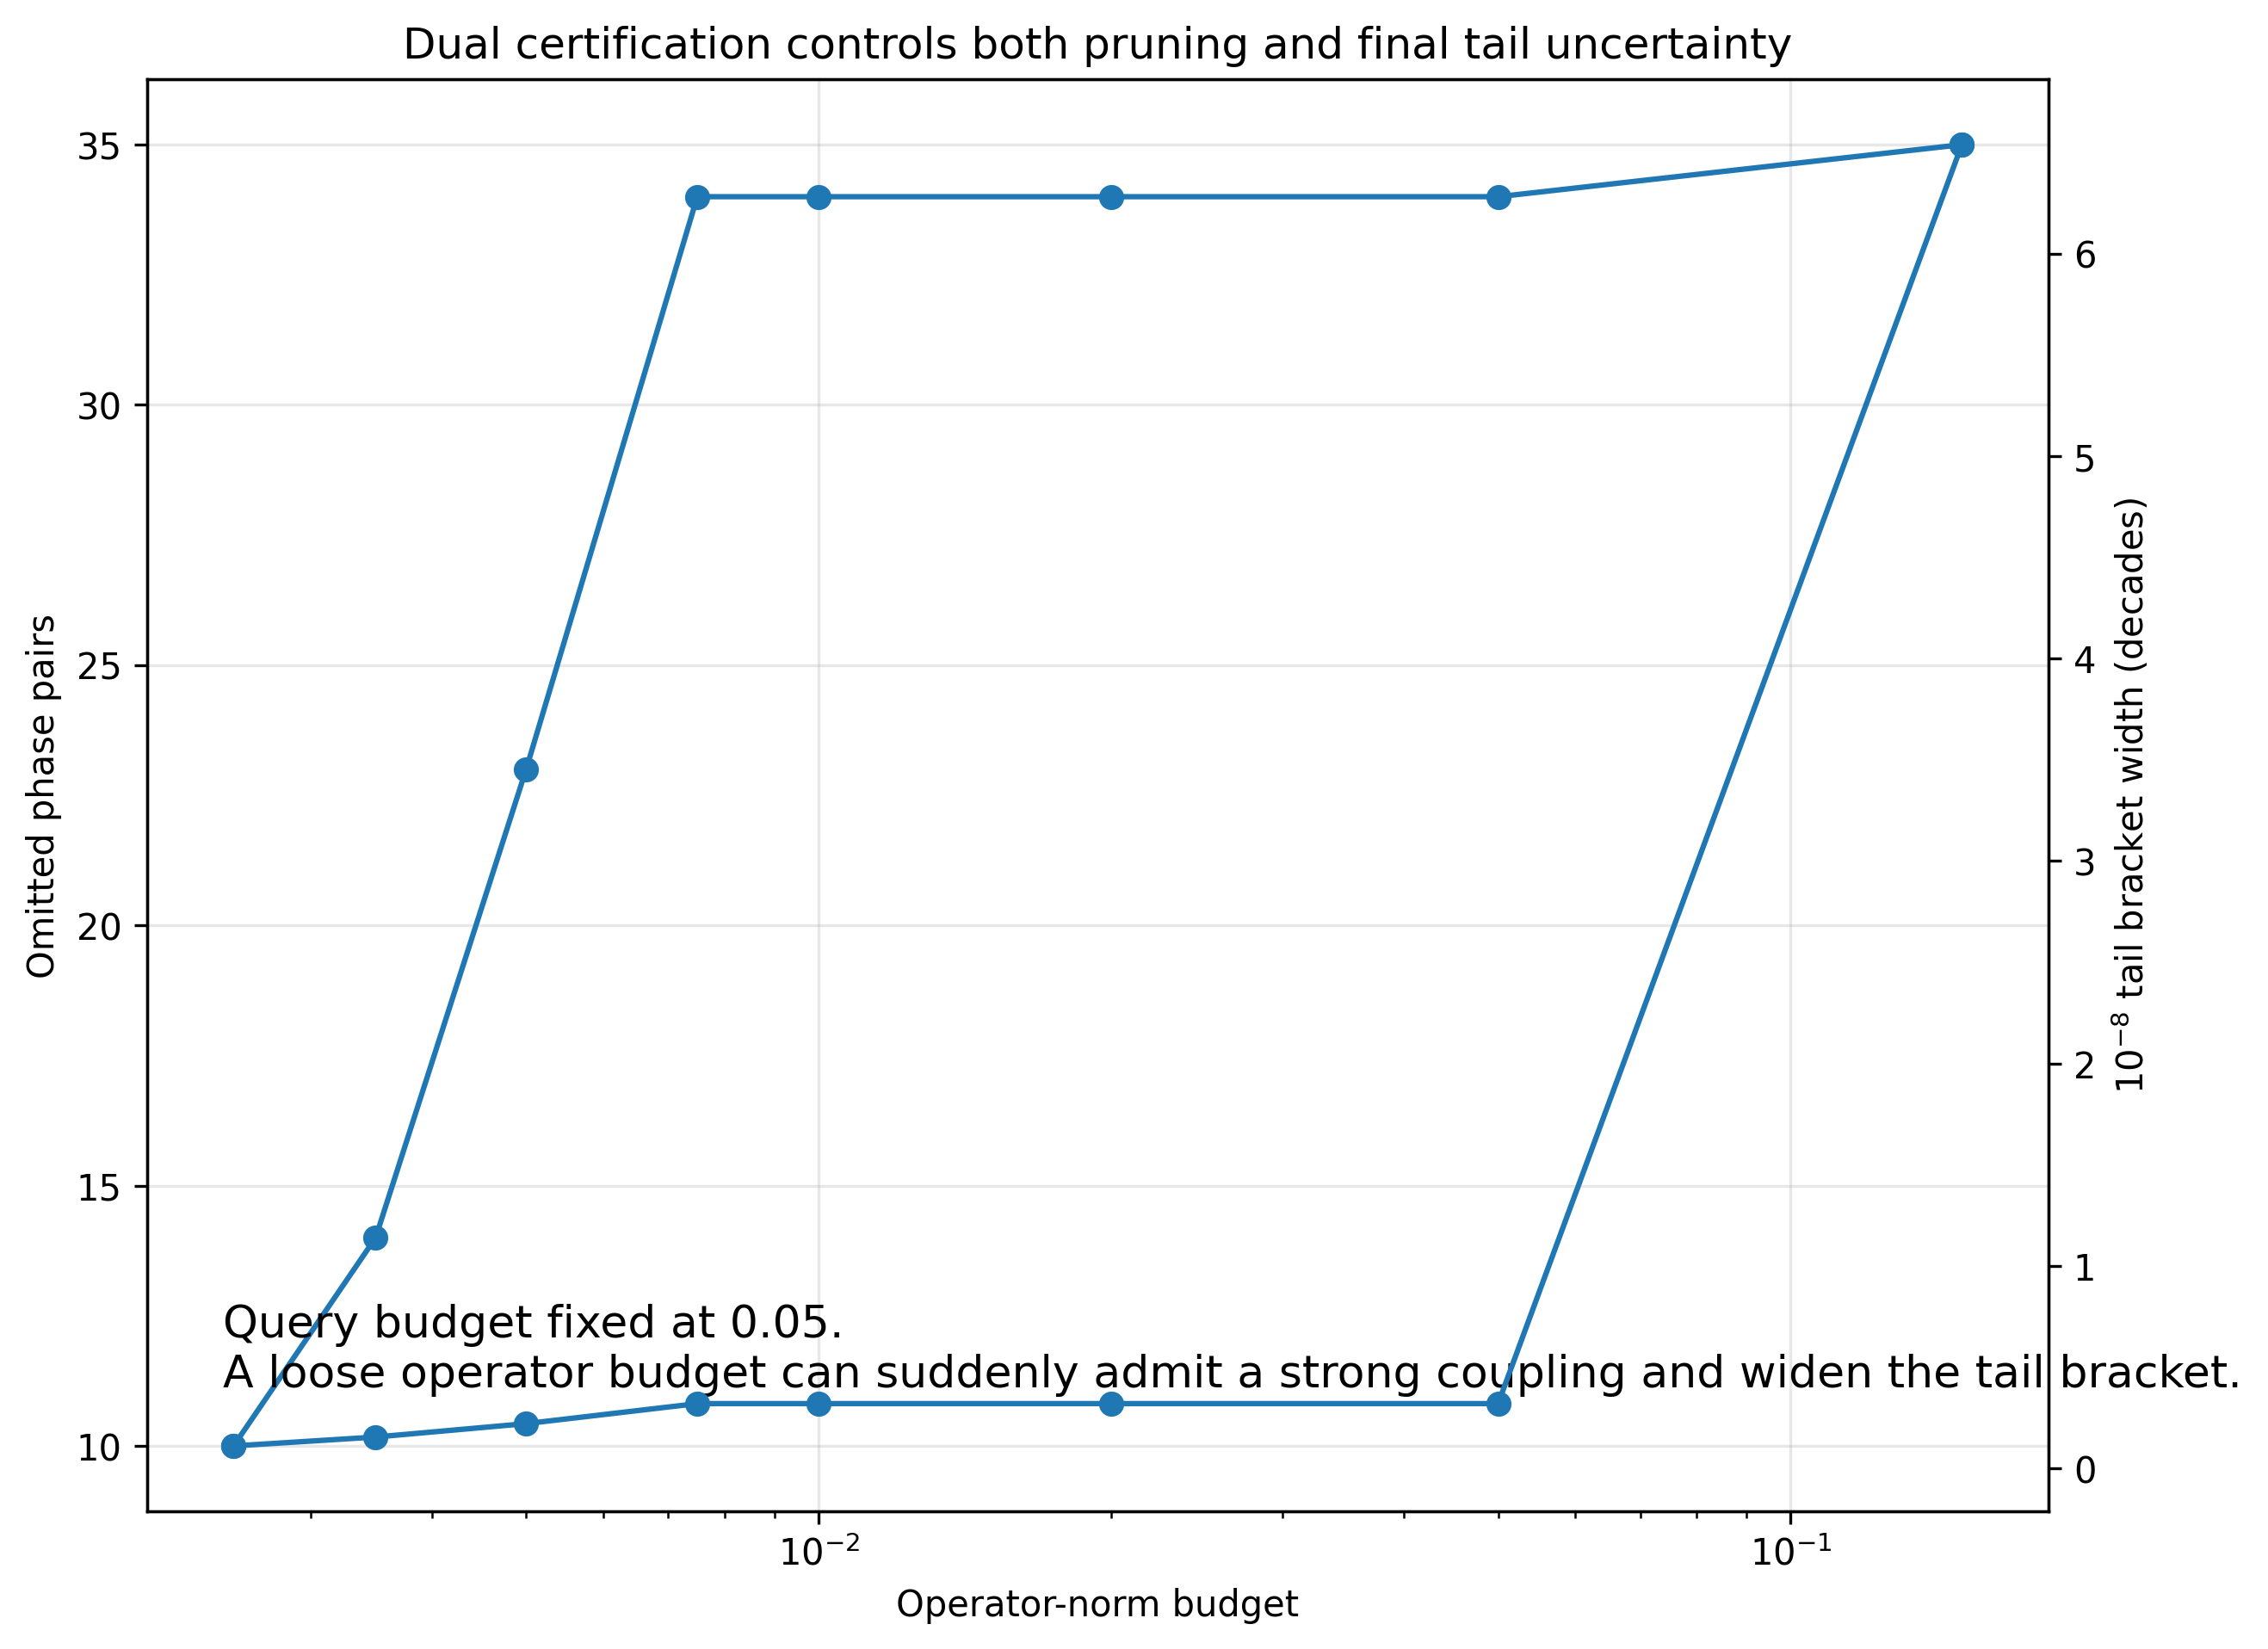
\includegraphics[width=.84\linewidth]{figure_14_dual_budget_tail_bridge.png}
\caption{Dual-budget phase pruning.  The query-local budget controls Krylov
propagation while the operator budget controls final spectral and tail
uncertainty.  A loose operator budget can admit a strong coupling and widen
the tail interval by several decades even when the Krylov-local budget still
passes.}
\label{fig:dual-budget-tail}
\end{figure}

In the deterministic ten-phase experiment, fixing the query budget at
\(0.05\) and the operator budget at \(0.005\) removed \(23\) of \(45\)
undirected phase pairs.  At a true probability of \(10^{-8}\), the certified
tail interval was
\[
10^{-8.11143}
\le
p
\le
10^{-7.89036},
\]
a width of about \(0.221\) decades.  With an operator budget of \(0.0075\),
\(34\) pairs were removed and the interval widened to about \(0.320\)
decades.  By contrast, allowing a strong coupling to be removed under a very
loose operator budget produced a multi-decade interval.

\subsection{Certify after prune}

There is a second route that does not use the pruned operator as the final
spectral approximation.  Let \(U\) be any orthonormal sample-space basis,
possibly generated cheaply from a pruned or approximate Krylov process, and
define
\[
B=U^\top A,
\qquad
F=(I-UU^\top)A,
\qquad
\delta=\|F\|_2.
\]

\begin{theorem}[Range-core singular-value certificate]
Let the singular values of \(A\) be \(\sigma_i(A)\), and let
\(\widetilde\sigma_i(B)\) denote the singular values of \(B\) padded by zeros
to the ambient spectral dimension.  Then
\[
\boxed{
\left|
\sigma_i(A)
-
\widetilde\sigma_i(B)
\right|
\le
\delta.
}
\]
Consequently,
\[
\max\{0,\widetilde\sigma_i(B)-\delta\}^2
\le
\lambda_i(AA^\top)
\le
\left(
\widetilde\sigma_i(B)+\delta
\right)^2.
\]
\end{theorem}

\begin{proof}
Because \(U\) has orthonormal columns,
\[
A=UB+F
\]
and
\[
\|A-UB\|_2=\|F\|_2=\delta.
\]
The nonzero singular values of \(UB\) are exactly those of \(B\).
The standard singular-value perturbation inequality gives the stated bound.
Squaring the nonnegative endpoints gives the eigenvalue interval.
\end{proof}

This provides a useful architecture:
\[
\boxed{
\text{pruned operator for basis discovery}
\to
\text{one exact streamed factor check}
\to
\text{certified spectral core}.
}
\]

\subsection{A retained negative result}

The preceding theorem is exact, but a correct interval need not be useful.

In a full-rank \(50\times50\) stress test, a pruned Krylov basis of dimensions
\(12\) through \(48\) left range residuals between roughly \(0.87\) and
\(0.99\) times the leading singular value.  The corresponding \(10^{-8}\)
tail intervals were therefore vacuous or thousands of decades wide.  At
dimension \(50\), the range residual fell to approximately
\(1.2\times10^{-15}\), and the tail interval collapsed to the exact value.

\begin{figure}[H]
\centering
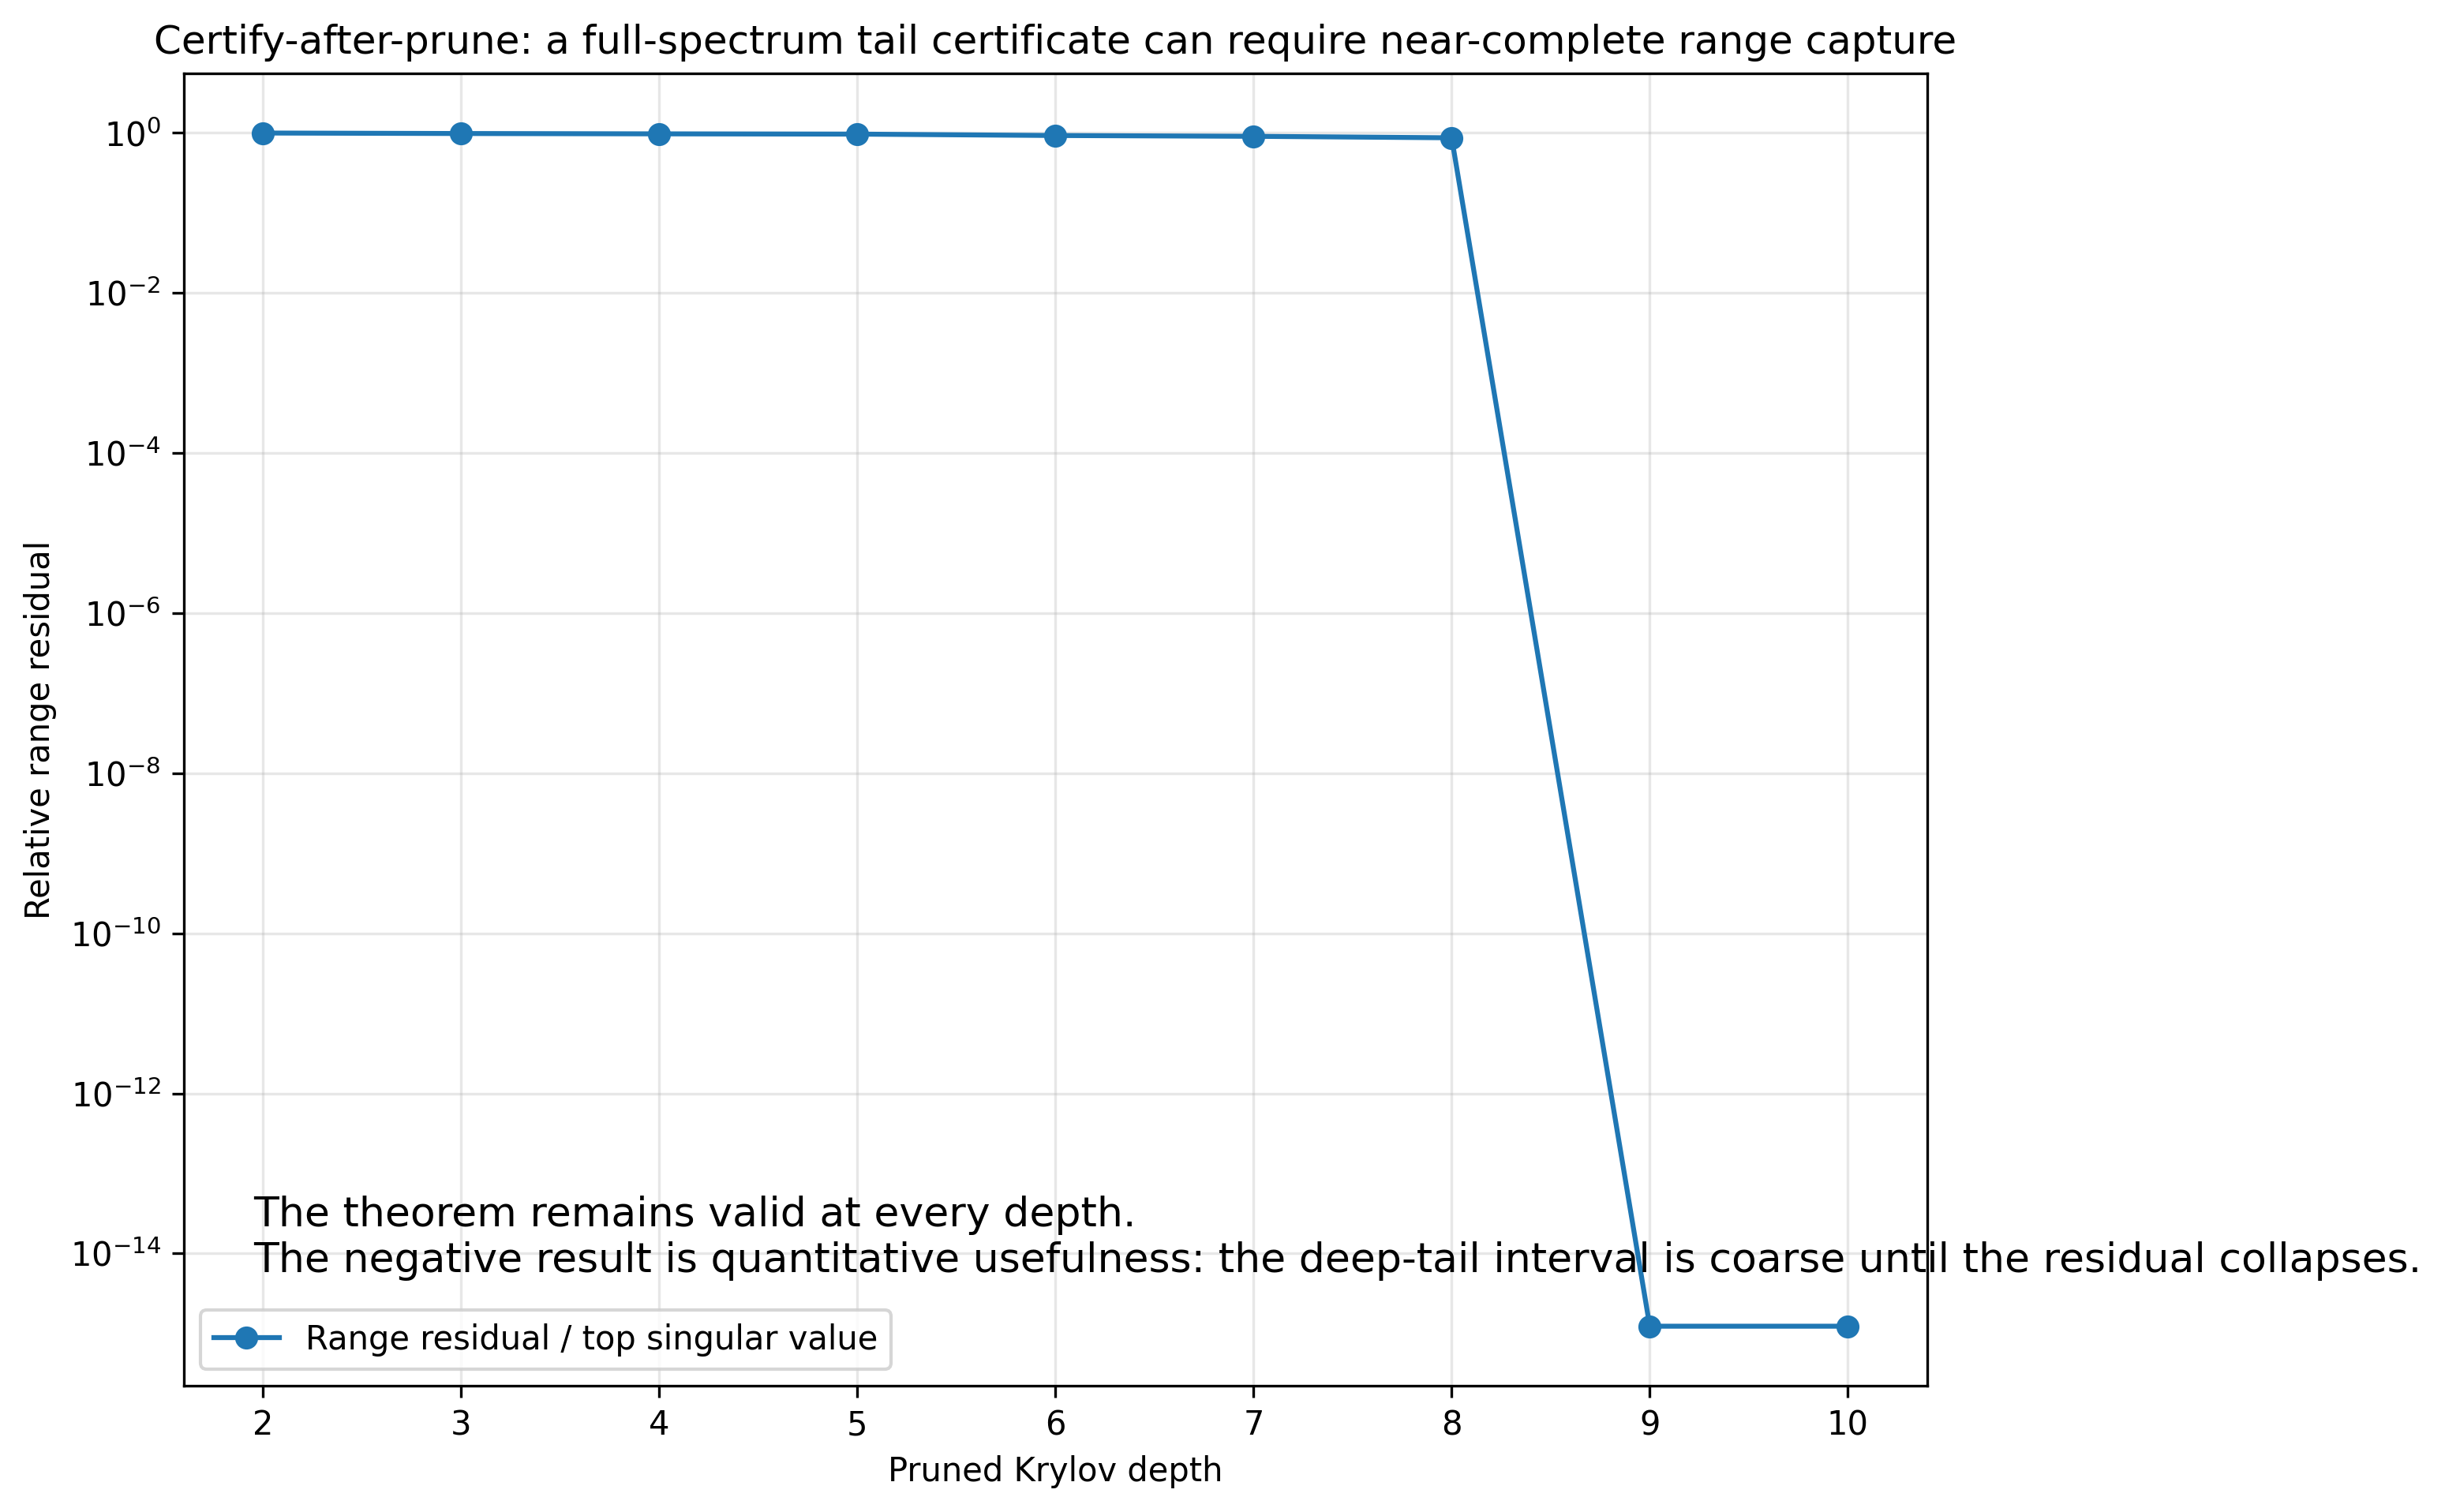
\includegraphics[width=.84\linewidth]{figure_15_range_core_certification.png}
\caption{Certify-after-prune range residual.  The range-core theorem is valid
at every depth, but a deep-tail full-spectrum guarantee can remain useless
until the range residual is genuinely small.  This negative result is retained
as a stopping-rule lesson rather than hidden as an implementation failure.}
\label{fig:range-core-cert}
\end{figure}

The practical lesson is that range-core certification is a stopping test, not
a promise that a severely incomplete basis automatically yields a useful
full-spectrum tail bound.


\section{Trace-aware residual certification and exact completion}

The spectral bridge in the preceding section used an operator-norm residual as
if every unresolved coefficient could move independently by the same amount.
That is rigorous but unnecessarily pessimistic once a nontrivial range basis
has already been captured.  The residual has considerably more structure.

Let \(U\in\mathbb R^{n\times r}\) have orthonormal columns and define
\[
B=U^\top A,
\qquad
F=(I-UU^\top)A.
\]
Then
\[
A=UB+F,
\qquad
U^\top F=0.
\]

\begin{theorem}[Exact core--residual decomposition]
\[
\boxed{
A^\top A
=
B^\top B+F^\top F.
}
\]
In particular the unresolved spectral term
\[
R=F^\top F
\]
is positive semidefinite.
\end{theorem}

\begin{proof}
Expand \((UB+F)^\top(UB+F)\).  The two cross terms vanish because
\(U^\top F=0\), while \(U^\top U=I\).
\end{proof}

This changes the certification problem.  Instead of an arbitrary Hermitian
error, the missing term is a positive residual with measurable spectral
moments.  Define
\[
t=\operatorname{tr}R,
\qquad
v=\operatorname{tr}(R^2),
\qquad
\rho=\|R\|_2.
\]
Then
\[
\boxed{
 t=\|F\|_F^2,
 \qquad
 v=\|FF^\top\|_F^2,
 \qquad
 \rho=\|F\|_2^2.
}
\]
The first quantity is the exact missing mean of the Gaussian quadratic form;
the second records how concentrated the residual spectrum is; the third is its
largest possible coefficient.

\subsection{A trace--Frobenius--cap MGF envelope}

Set
\[
C=B^\top B,
\qquad
H=C+R,
\qquad
c=\lambda_{\max}(C).
\]
For \(0<2\theta(c+\rho)<1\), put
\[
\alpha=(1-2\theta c)^{-1}.
\]

\begin{theorem}[Trace--Frobenius--cap log-MGF certificate]
For the Gaussian quadratic form with coefficient matrix \(H\),
\[
K_H(\theta)
=-\frac12\log\det(I-2\theta H)
\]
satisfies
\[
\boxed{
K_H(\theta)
\le
K_C(\theta)
+
\theta\alpha t
+
\frac{\theta^2\alpha^2v}
     {1-2\theta\alpha\rho}.
}
\]
\end{theorem}

\begin{proof}
Factor the determinant through the known core:
\[
I-2\theta(C+R)
=
(I-2\theta C)^{1/2}
(I-2\theta T)
(I-2\theta C)^{1/2},
\]
where
\[
T=(I-2\theta C)^{-1/2}
R
(I-2\theta C)^{-1/2}.
\]
Since
\[
\|(I-2\theta C)^{-1/2}\|_2^2=\alpha,
\]
we have
\[
\operatorname{tr}T\le\alpha t,
\qquad
\operatorname{tr}(T^2)\le\alpha^2v,
\qquad
\|T\|_2\le\alpha\rho.
\]
For every eigenvalue \(x\) of \(T\),
\[
-\frac12\log(1-2\theta x)
\le
\theta x
+
\frac{\theta^2x^2}
     {1-2\theta\alpha\rho}.
\]
The scalar inequality follows from the power series of \(-\log(1-u)\) and a
geometric bound on all terms of degree at least two.  Summing over the
eigenvalues of \(T\) proves the result.
\end{proof}

\begin{corollary}[Trace-aware Chernoff upper tail]
For \(Q=Z^\top HZ\) with \(Z\sim N(0,I)\),
\[
\boxed{
\Pr(Q\ge q)
\le
\inf_{0<2\theta(c+\rho)<1}
\exp\{\widehat K_H(\theta)-\theta q\},
}
\]
where \(\widehat K_H\) is the preceding MGF upper bound.
\end{corollary}

A complementary lower endpoint is immediate from
\[
H=C+R\succeq C.
\]
Using the same normal vector,
\[
Z^\top HZ\ge Z^\top CZ
\]
almost surely, and therefore
\[
\boxed{
\Pr(Z^\top CZ\ge q)
\le
\Pr(Z^\top HZ\ge q).
}
\]
The lower endpoint can be evaluated by K-COS on the captured core spectrum,
while the upper endpoint is obtained from the optimized trace-aware Chernoff
bound.

\subsection{Finite stress test}

The previous coefficient-wise Weyl interval was intentionally conservative.
On the same full-rank, 50-dimensional stress test used in the preceding
section, its \(10^{-8}\) tail interval remained thousands of decades wide
until essentially the complete range had been captured.  Preserving the exact
residual trace and higher residual moments changes that behavior substantially.

\begin{table}[H]
\centering
\caption{Tail-bracket width at a true probability of \(10^{-8}\).  The
trace/moment certificate is still conservative, but it is orders of magnitude
narrower than coefficient-wise Weyl inflation before full range capture.}
\begin{tabular}{rrrr}
\toprule
Krylov depth & basis dimension & v0.7 Weyl width & v0.8 moment width\\
\midrule
4 & 24 & 90,097 & 11.86\\
5 & 30 & 16,511 & 9.76\\
6 & 36 & 3,747 & 7.67\\
7 & 42 & 2,275 & 5.70\\
8 & 48 & 1,165 & 3.39\\
\bottomrule
\end{tabular}
\end{table}

\begin{figure}[H]
\centering
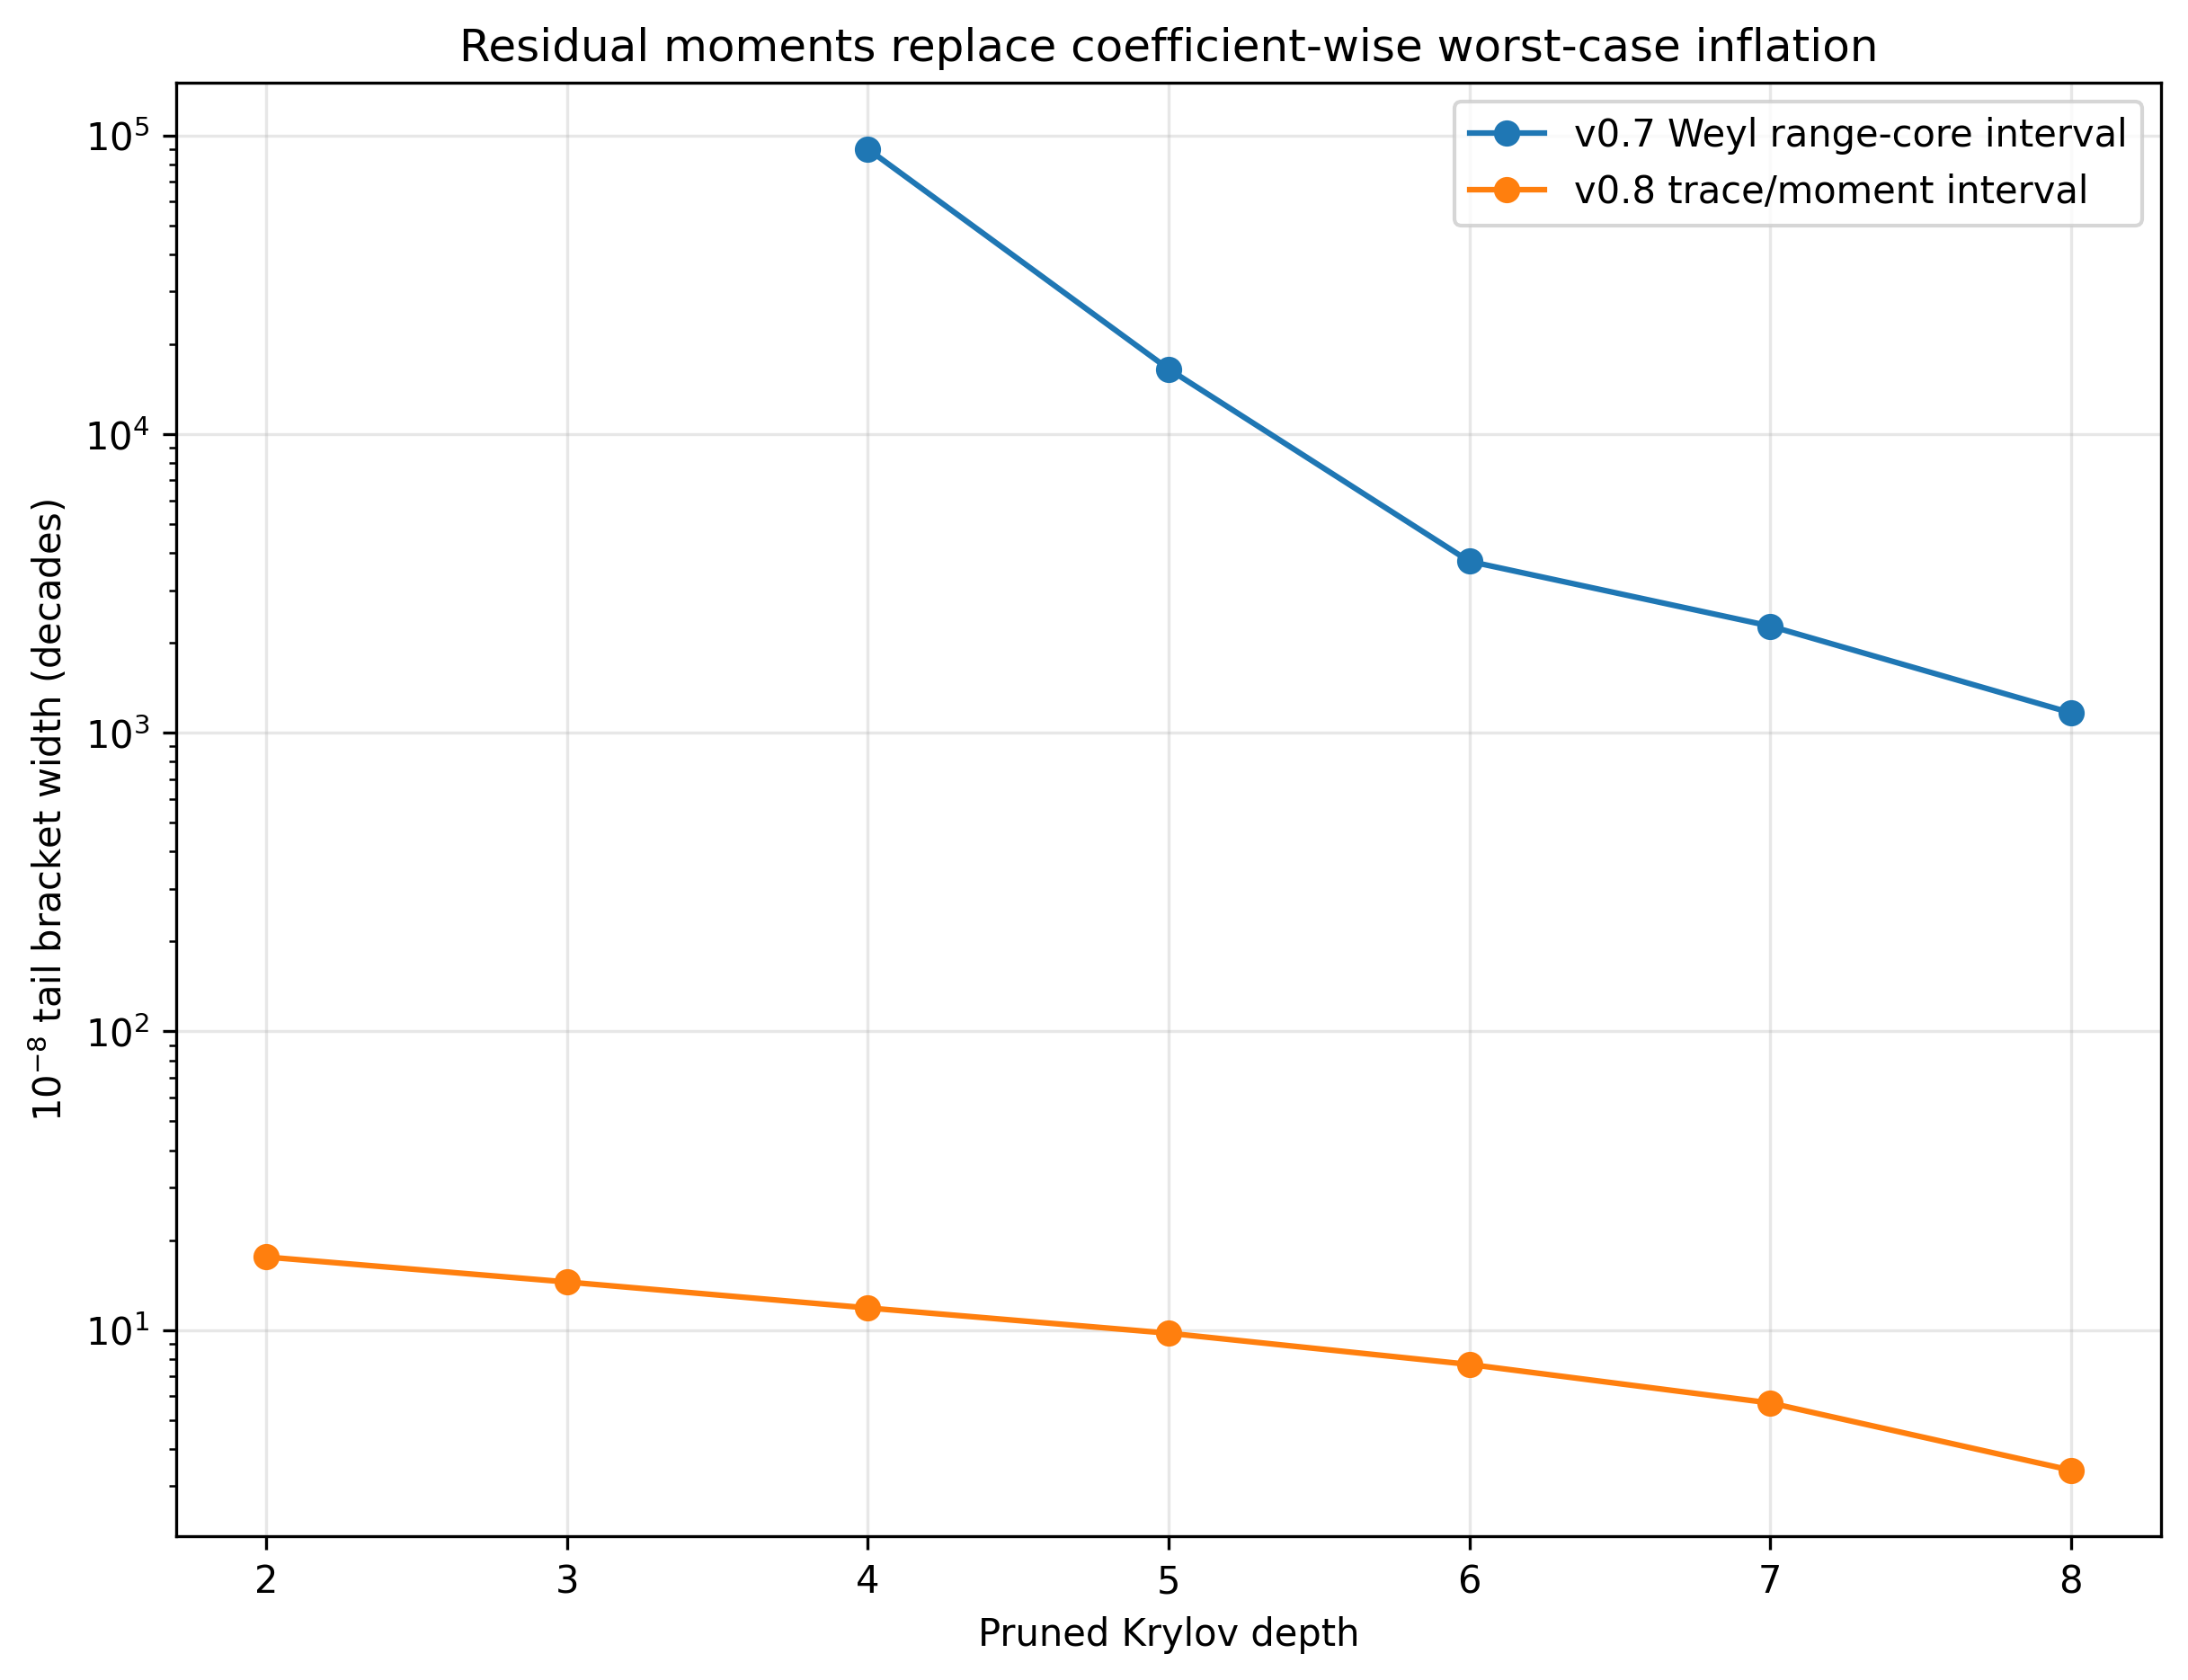
\includegraphics[width=.84\linewidth]{figure_16_trace_moment_vs_weyl.png}
\caption{Incomplete-range tail certification before exact completion.  The
trace/moment bound preserves the amount and concentration of unresolved
spectral mass instead of shifting every coefficient by one worst-case radius.}
\label{fig:trace-moment-vs-weyl}
\end{figure}

A separate random implementation audit used 120 random factor/range pairs and
four admissible positive tilts per pair, for 480 MGF comparisons.  Both the
trace/cap and trace--Frobenius--cap envelopes dominated the exact log MGF in
every tested case.  The trace--Frobenius--cap form was at least as tight as the
trace/cap form in approximately 83.5\% of those comparisons.  This finite
sweep audits the implementation; the theorem above supplies the universal
argument.

\subsection{Residual rank from moments}

The same invariants determine when it is better to stop approximating the
missing spectrum and complete it exactly.  Let
\[
s=\operatorname{rank}F=\operatorname{rank}R.
\]
If the nonzero eigenvalues of \(R\) are \(r_1,\ldots,r_s\), then
\[
t=\sum_i r_i,
\qquad
v=\sum_i r_i^2,
\qquad
r_i\le\rho.
\]

\begin{theorem}[Residual-rank bracket]
\[
\boxed{
\left\lceil
\max\left\{
\frac{t}{\rho},
\frac{t^2}{v}
\right\}
\right\rceil
\le
\operatorname{rank}F
\le
n-r.
}
\]
The zero-residual case is interpreted separately as rank zero.
\end{theorem}

\begin{proof}
The inequality \(t\le s\rho\) gives \(s\ge t/\rho\).  Cauchy--Schwarz gives
\[
t^2
=
\left(\sum_{i=1}^s r_i\right)^2
\le
s\sum_{i=1}^s r_i^2
=sv,
\]
so \(s\ge t^2/v\).  Finally, every column of \(F\) lies in
\(\operatorname{range}(U)^\perp\), whose dimension is \(n-r\).
\end{proof}

Whenever the integer lower bound equals \(n-r\), the missing rank is certified
exactly without computing a residual SVD.

\begin{figure}[H]
\centering
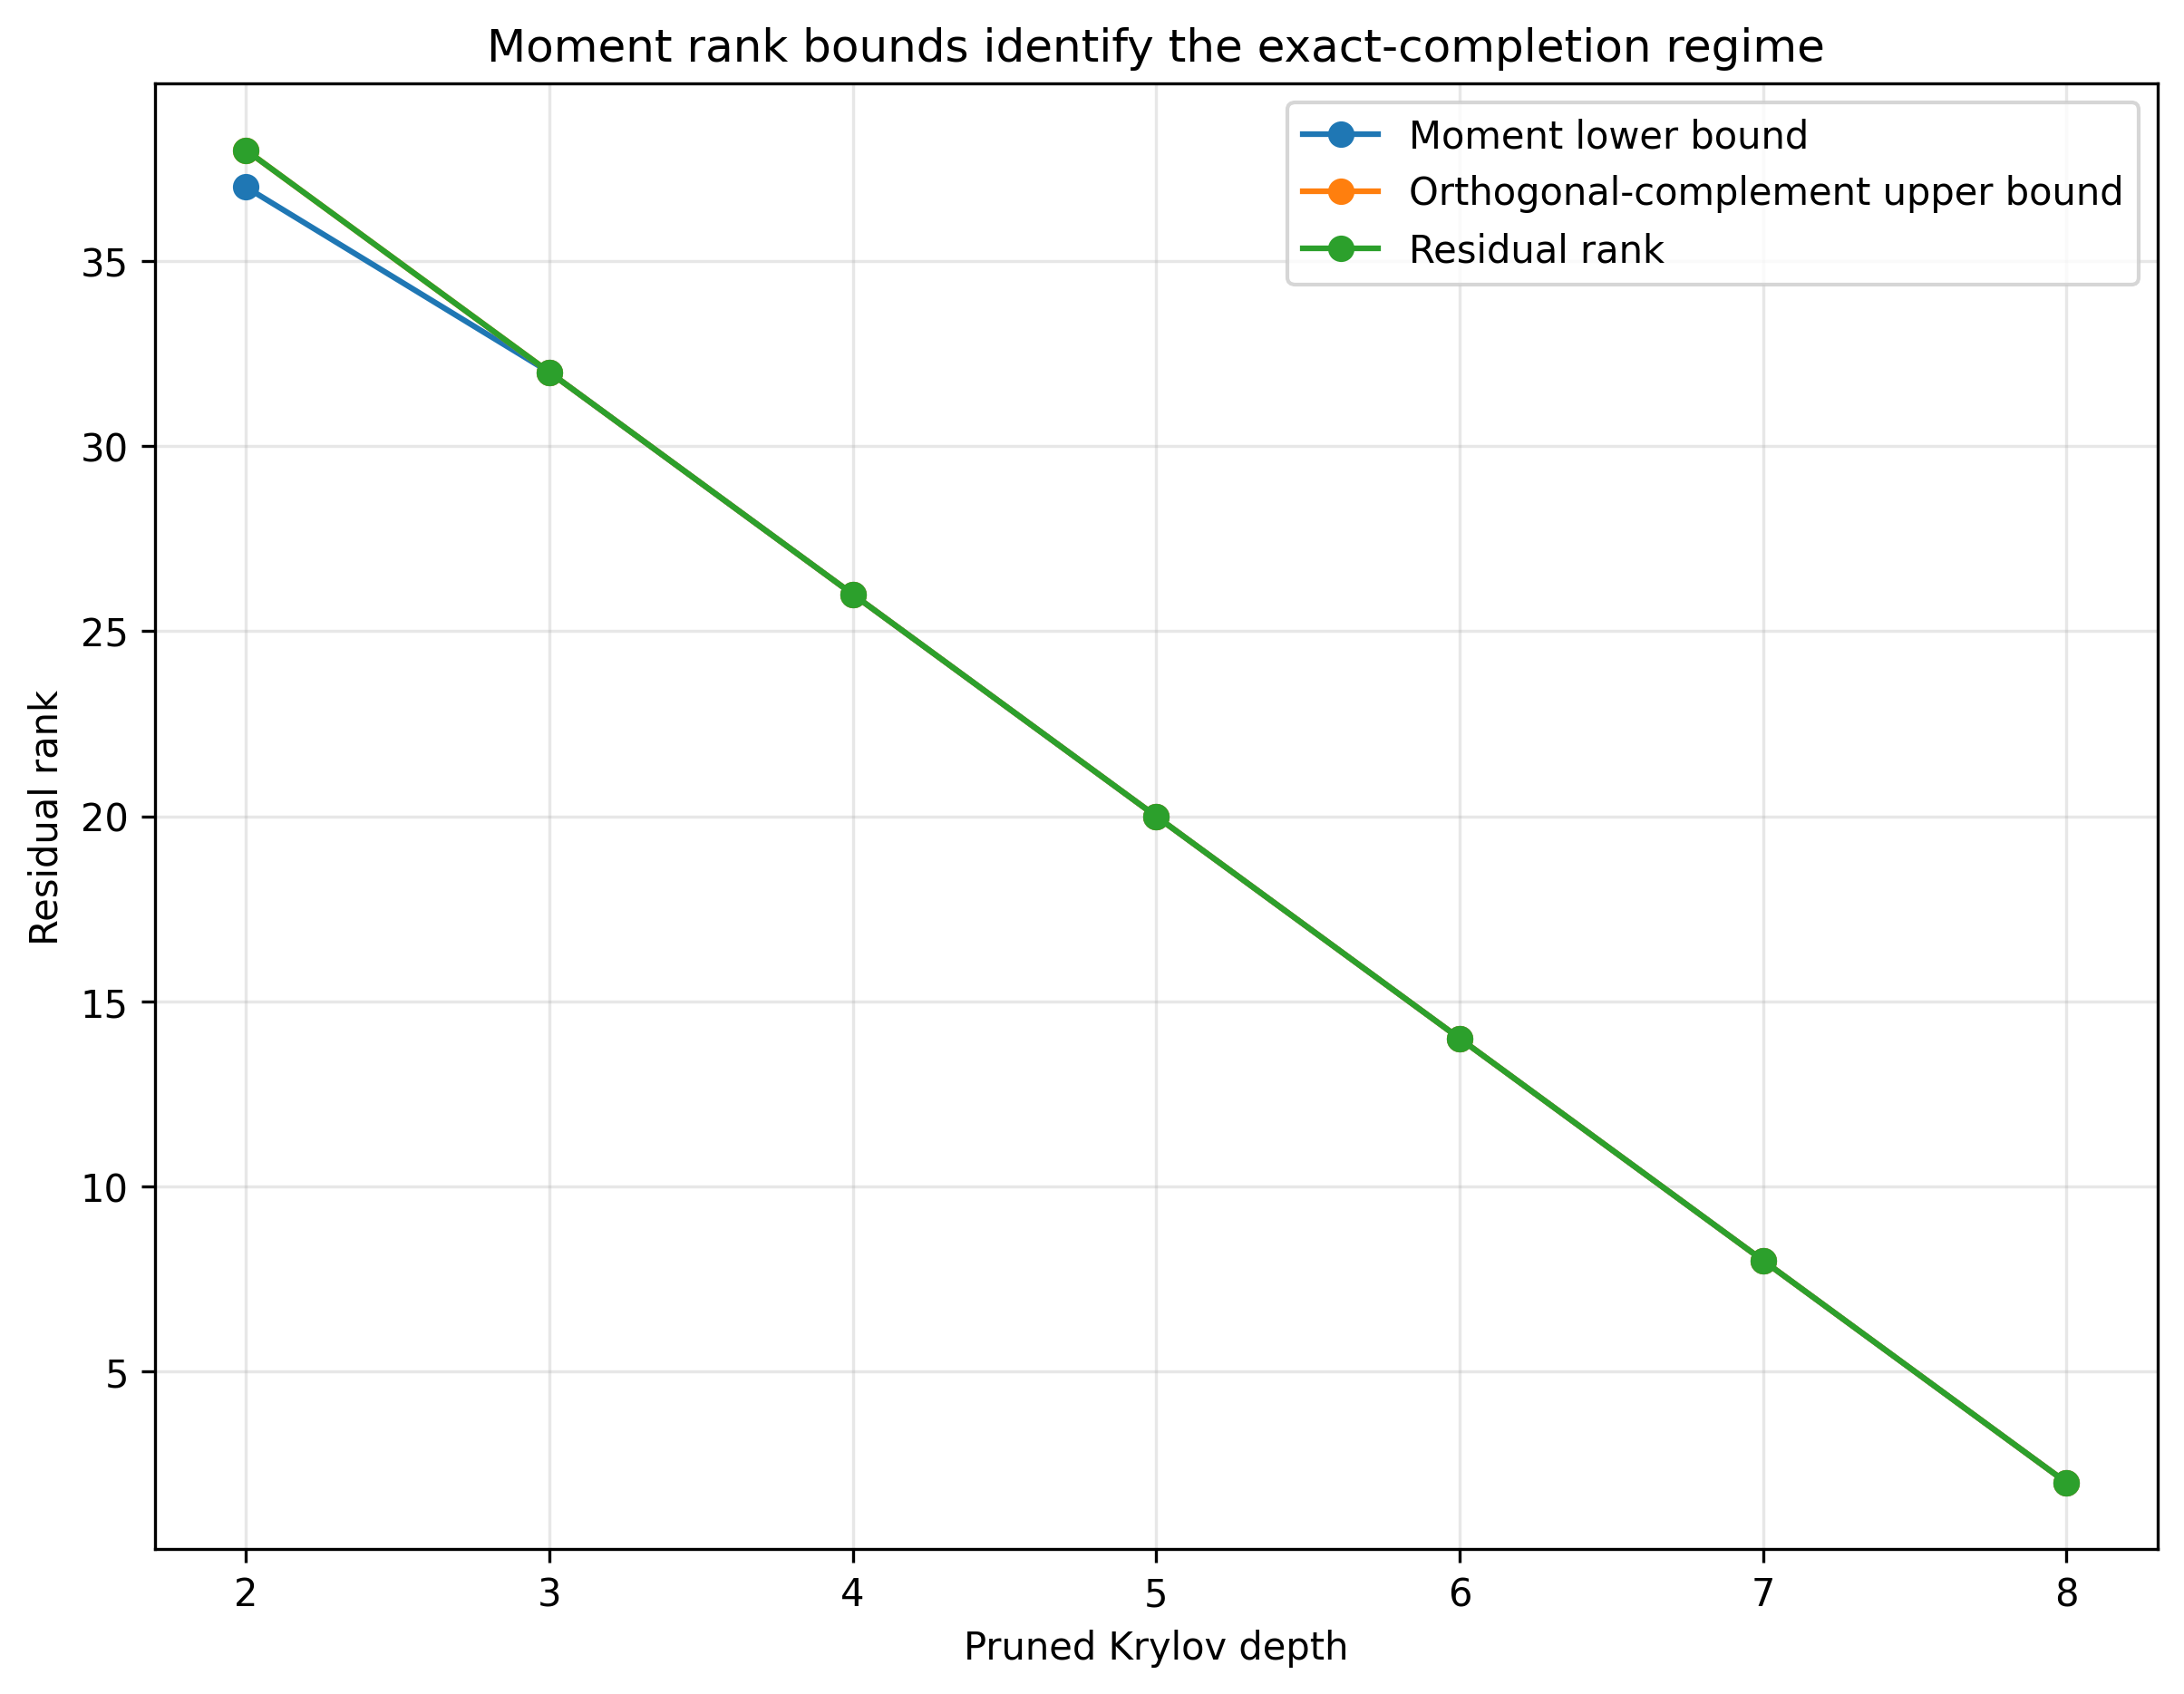
\includegraphics[width=.84\linewidth]{figure_17_residual_rank_completion.png}
\caption{Residual-rank certification in the full-rank stress test.  From depth
3 onward the moment lower bound meets the orthogonal-complement upper bound.
At depth 8 exactly two residual directions remain.}
\label{fig:residual-rank-completion}
\end{figure}

\subsection{Exact residual completion}

Suppose a compact factorization of the residual is
\[
F=WD,
\]
where \(W\) has orthonormal columns.  Since \(F\) lies in the orthogonal
complement of \(U\),
\[
U^\top W=0.
\]

\begin{theorem}[Exact residual completion]
\[
\boxed{
A
=
[U\;W]
\begin{bmatrix}
B\\D
\end{bmatrix}.
}
\]
Consequently, the nonzero singular values of \(A\) are exactly the singular
values of the stacked completion core
\[
\mathcal C_{\rm complete}
=
\begin{bmatrix}
B\\D
\end{bmatrix}.
\]
\end{theorem}

This identity admits a column-streamed implementation.  For each residual
column block, project against the residual basis accumulated so far, append
only genuinely new directions through rank-revealing QR or SVD, and extend the
coordinate matrices of earlier blocks with zero rows.  New residual directions
are orthogonal to every earlier residual block by construction, so no earlier
data block must be revisited.

In the deterministic stress test, exact residual completion reproduced the
full singular spectrum at relative errors between approximately
\(2\times10^{-16}\) and \(6\times10^{-16}\) for all tested incomplete bases.
The resulting \(10^{-8}\) tail differed from the full-spectrum reference by
less than \(10^{-14}\) decades.  At depth 8 the candidate range had dimension
48, the missing rank was certified as exactly two, and appending those two
residual directions closed the spectrum without another approximate Krylov
stage.

\subsection{Hybrid stopping rule}

The resulting production logic is not ``approximate forever.''  It is a
certified handoff between two regimes:
\[
\boxed{
\begin{array}{c}
\text{streamed / pruned Krylov}\\[2mm]
\downarrow\\[-1mm]
\text{residual moments }(t,v,\rho)\\[2mm]
\downarrow\\[-1mm]
\begin{cases}
\text{continue Krylov}, & \text{residual range still large},\\
\text{exact streamed residual completion}, & \text{completion rank affordable}.
\end{cases}
\end{array}
}
\]

The trace-aware tail certificate remains useful as a rigorous intermediate
bound and as a stopping diagnostic.  Once only a small number of residual
directions remain, exact completion is mathematically preferable to forcing a
worst-case tail envelope to become artificially sharp.

\section{Realistic rare-variant SKAT simulation validation}

The preceding sections establish operator identities and certified numerical
bounds.  This section tests the same machinery on the project's existing
rare-variant SKAT simulation layer, including explicit LD structure,
covariates, per-variant standardization, rare-variant weighting, and the
phenotype-space score statistic.

\subsection{Simulation provenance and a corrected historical defect}

Two established genotype generators were used.

The first is a latent-Gaussian block-LD generator.  Within a genomic block,
alleles are obtained by thresholding correlated Gaussian latent variables at
variant-specific minor-allele frequencies.

The second is a copy-LD generator in which haplotype states persist along a
block with high probability and are occasionally redrawn.  During the v0.9
audit, a defect was found in the historical implementation: the genotype
matrix was allocated with \verb|np.empty| and then updated using \verb|+=|.
Because the initial contents of \verb|np.empty| are unspecified, those old
copy-LD benchmark values are not reproducible evidence.  The v0.9 generator
uses an explicitly zero-initialized matrix before haplotype accumulation.
All copy-LD results reported below use the corrected implementation.

\subsection{Tested LD regimes}

Four deterministic scenarios were evaluated.

\begin{table}[H]
\centering
\caption{Realistic rare-variant simulation scenarios.  Adjacent $r^2$ is
computed within the simulated LD blocks after variant standardization.}
\begin{tabular}{lrrrrr}
\toprule
scenario & $n$ & $m$ & rank & median adjacent $r^2$ & effective rank\\
\midrule
latent LD, moderate & 600 & 3000 & 596 & 0.0069 & 441.9\\
latent LD, strong & 600 & 3000 & 596 & 0.1140 & 240.3\\
copy LD, strong & 600 & 3000 & 596 & 0.8298 & 200.1\\
copy LD, large & 1000 & 5000 & 996 & 0.8179 & 353.0\\
\bottomrule
\end{tabular}
\end{table}

The corresponding spectra therefore span a substantial range of concentration:
stronger LD reduces effective rank even when the nominal quadratic-form rank
remains close to the sample residual dimension.

\begin{figure}[H]
\centering
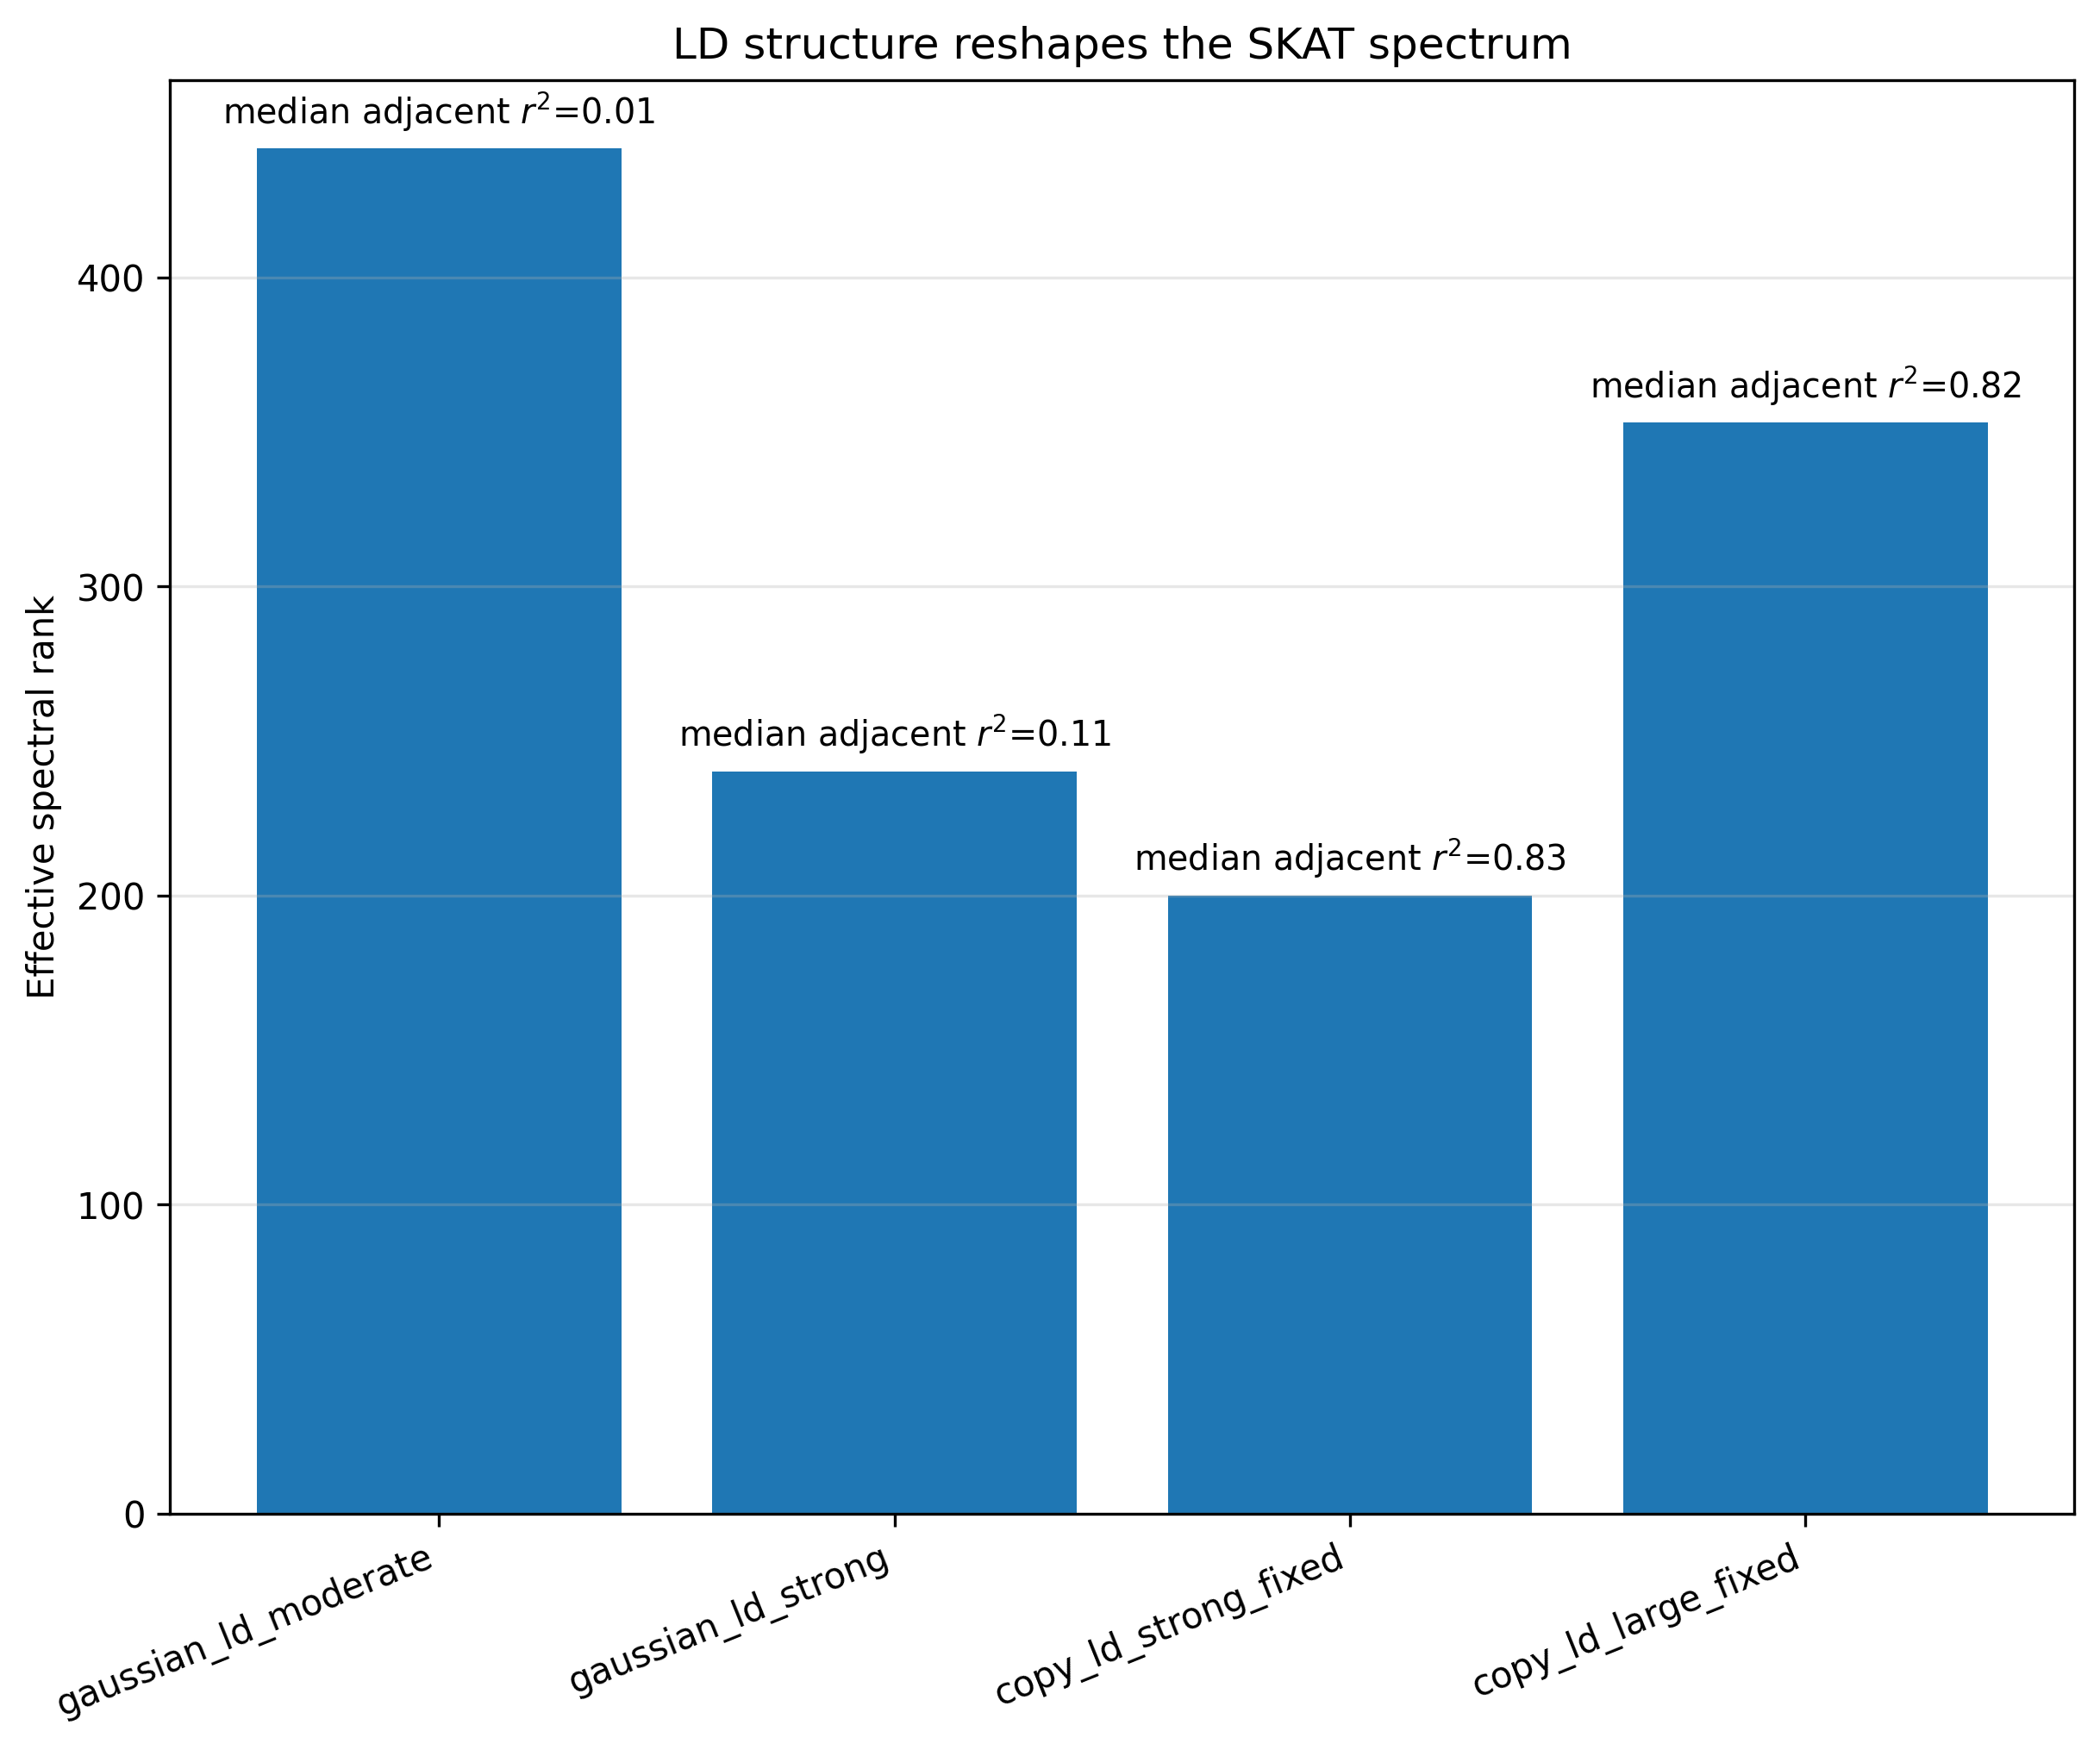
\includegraphics[width=.84\linewidth]{figure_18_realistic_ld_effective_rank.png}
\caption{LD structure changes the effective spectral rank.  The corrected
copy-LD models create much stronger local dependence than the latent-Gaussian
moderate-LD case, while all remain within the same streamed SKAT pipeline.}
\label{fig:realistic-ld-rank}
\end{figure}

\subsection{Streaming directly from raw genotype blocks}

The raw genotype matrix was streamed in resident variant blocks of widths
31, 127, and 509.  Within each block the implementation performs

\[
G_b
\to
G_b-\bar G_b
\to
\text{variance scaling}
\to
M_X G_b
\to
W_b^{1/2}
\to
A_bA_b^\top,
\]

without materializing the full weighted factor.

Across all four LD scenarios and all three resident block sizes, the largest
relative discrepancy against the fully materialized kernel was

\[
\boxed{6.61\times10^{-16}}.
\]

\begin{figure}[H]
\centering
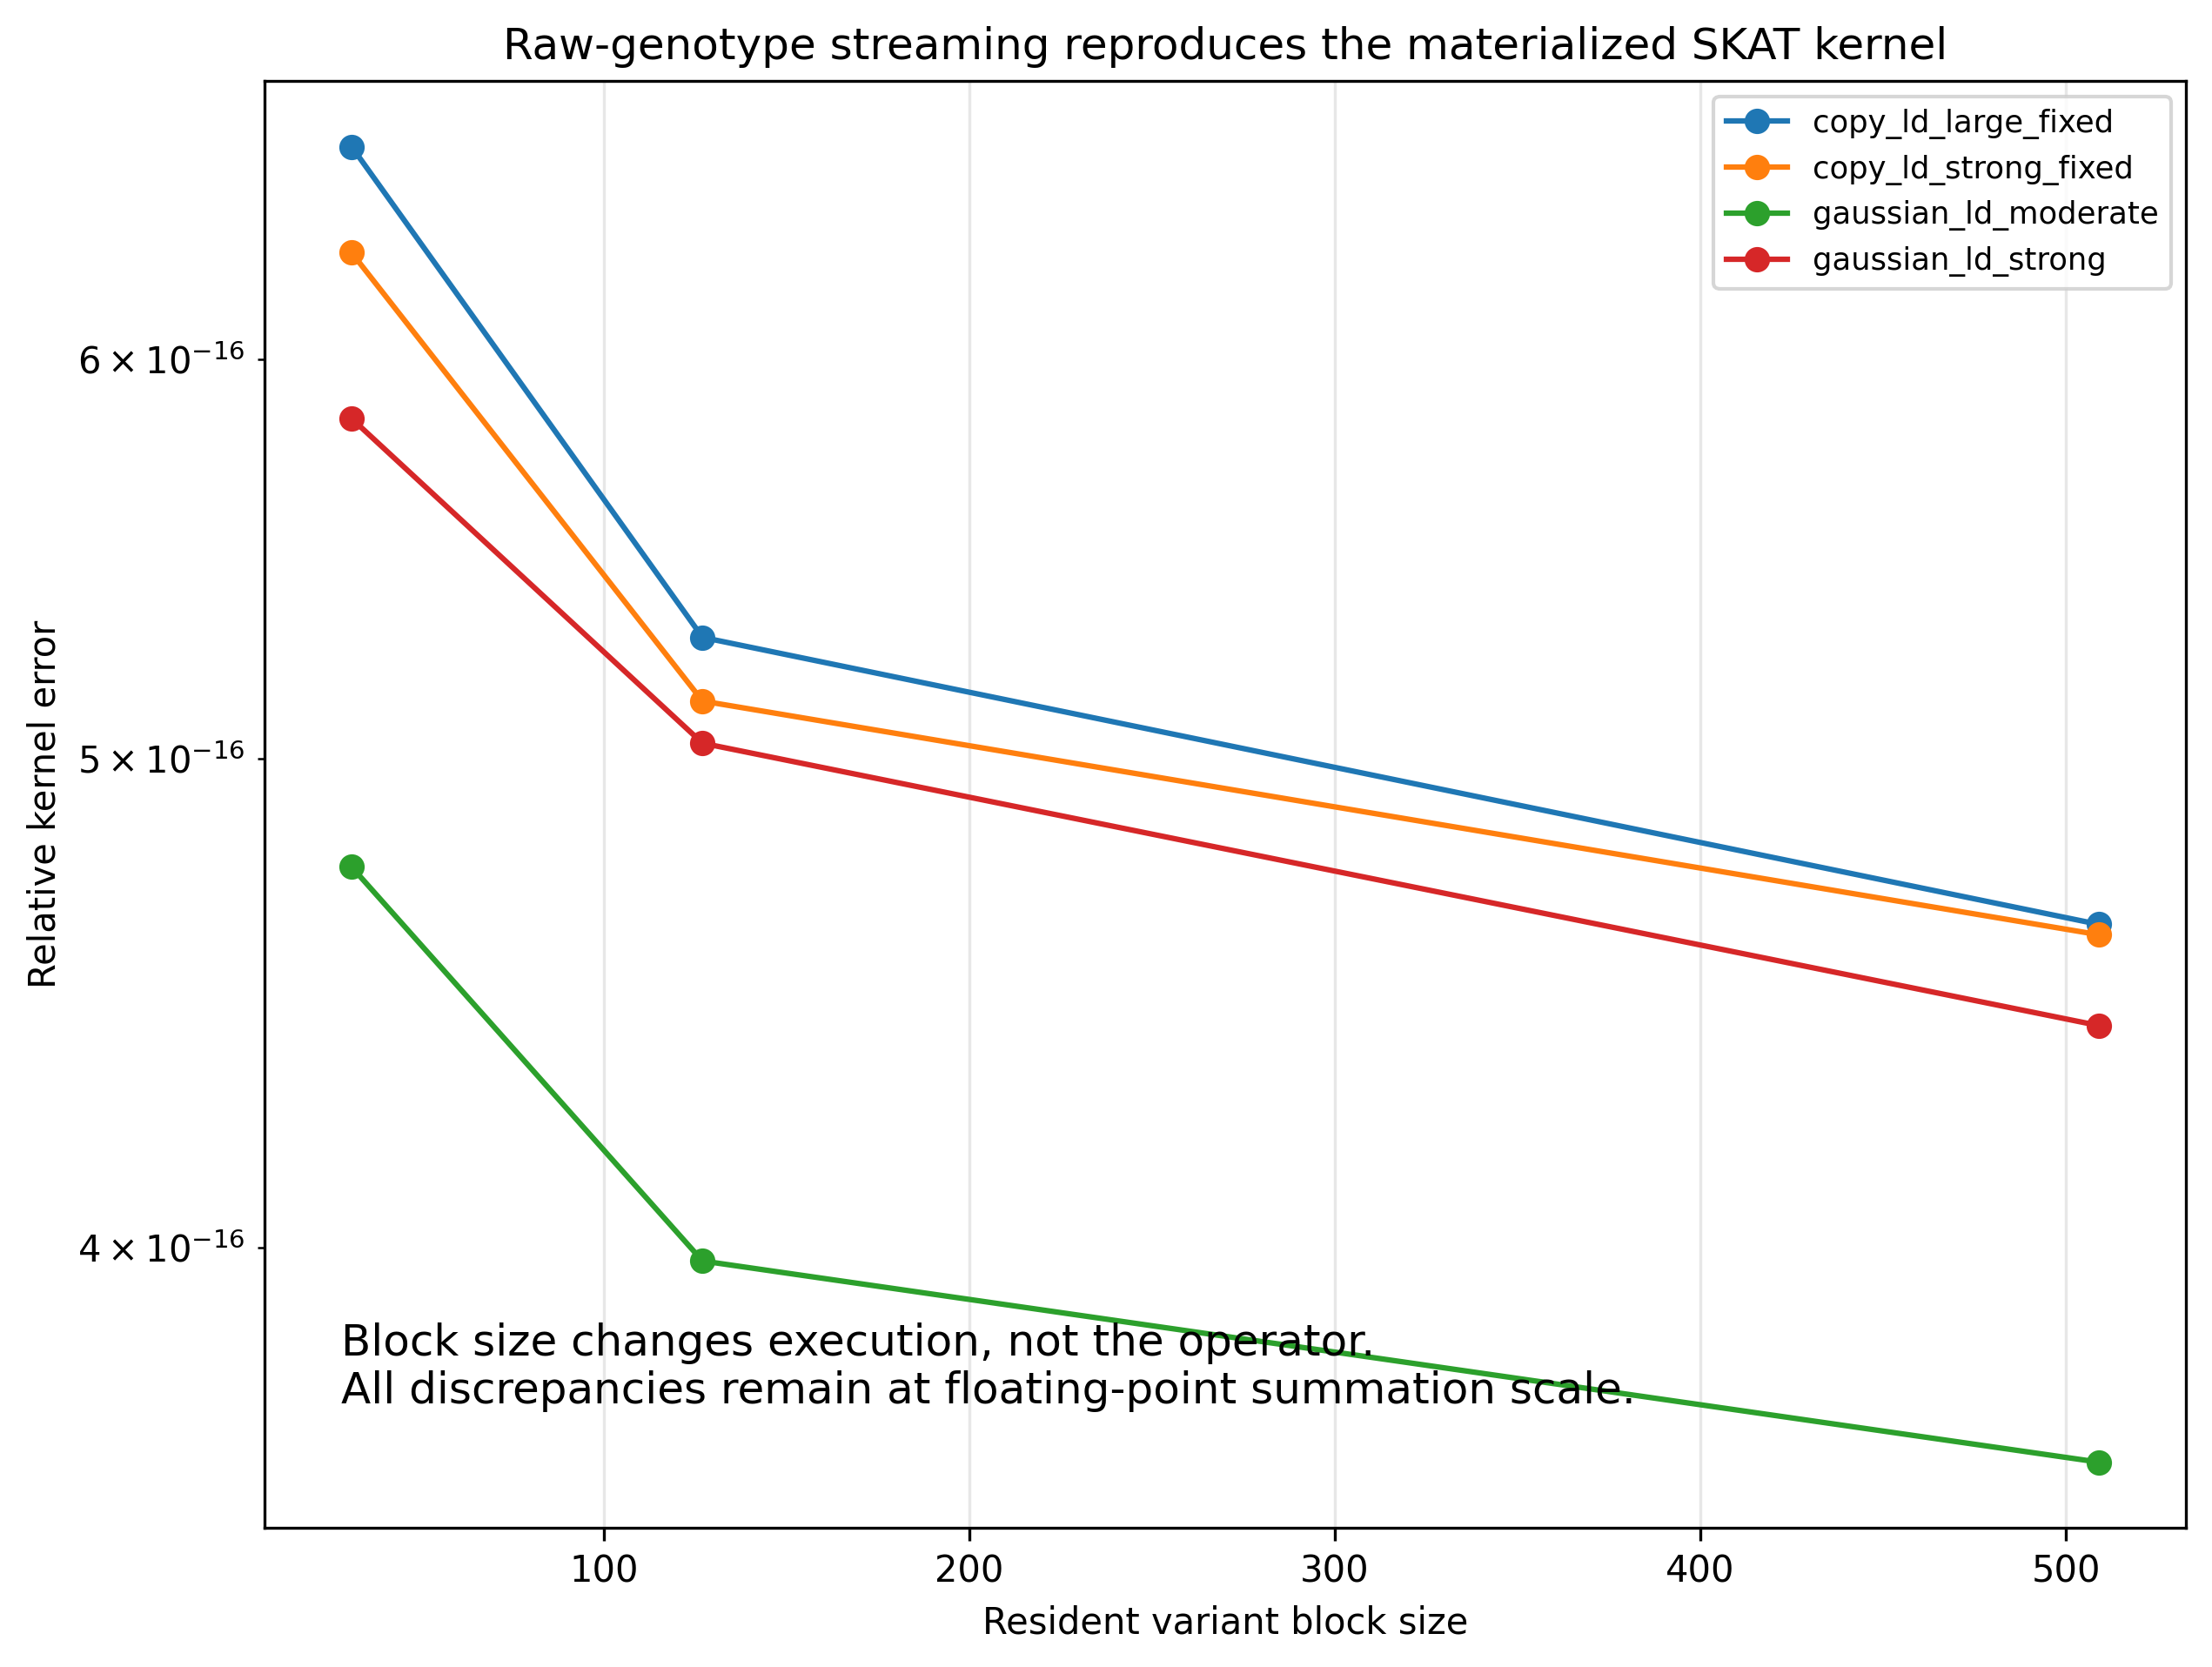
\includegraphics[width=.84\linewidth]{figure_19_realistic_streaming_invariance.png}
\caption{Raw-genotype streaming reproduces the materialized SKAT kernel across
multiple LD regimes and block sizes.  The observed discrepancies are at
floating-point summation scale.}
\label{fig:realistic-streaming}
\end{figure}

This test is stronger than applying the streamed identity to a precomputed
factor because the centering, variance scaling, covariate projection, and
rare-variant weights are all performed inside the block loop.

\subsection{Phenotype-space equivalence}

For each scenario, 100 Gaussian null residual draws were evaluated in three
ways:

\begin{enumerate}
\item directly through the factor,
\[
Q=\frac12\|A^\top e\|_2^2;
\]
\item through the sample kernel,
\[
Q=\frac12 e^\top Ke;
\]
\item through the eigencoordinates of $K$.
\end{enumerate}

The worst relative discrepancy across all draws and all scenarios was

\[
\boxed{8.32\times10^{-16}}.
\]

Thus the simulated phenotype path, the streamed kernel, and the generalized
$\chi^2$ spectral representation agree to floating-point precision.

\subsection{Deep tails on realistic LD spectra}

For every scenario, tail queries were generated at tilt fractions
0.90, 0.97, and 0.99 of the positive singularity.  K-COS was compared with a
higher-resolution full-spectrum tilted reference.

The large corrected copy-LD case was then pushed further, to fractions
0.995, 0.997, 0.999, and 0.9995.  The deepest tested reference value was

\[
\boxed{\log_{10}p=-457.973916}.
\]

At that point the displayed K-COS and high-resolution full-spectrum values
were identical.  Across the complete realistic-LD battery, the largest
absolute discrepancy was

\[
\boxed{3.21\times10^{-12}\ \text{decades}}.
\]

\begin{figure}[H]
\centering
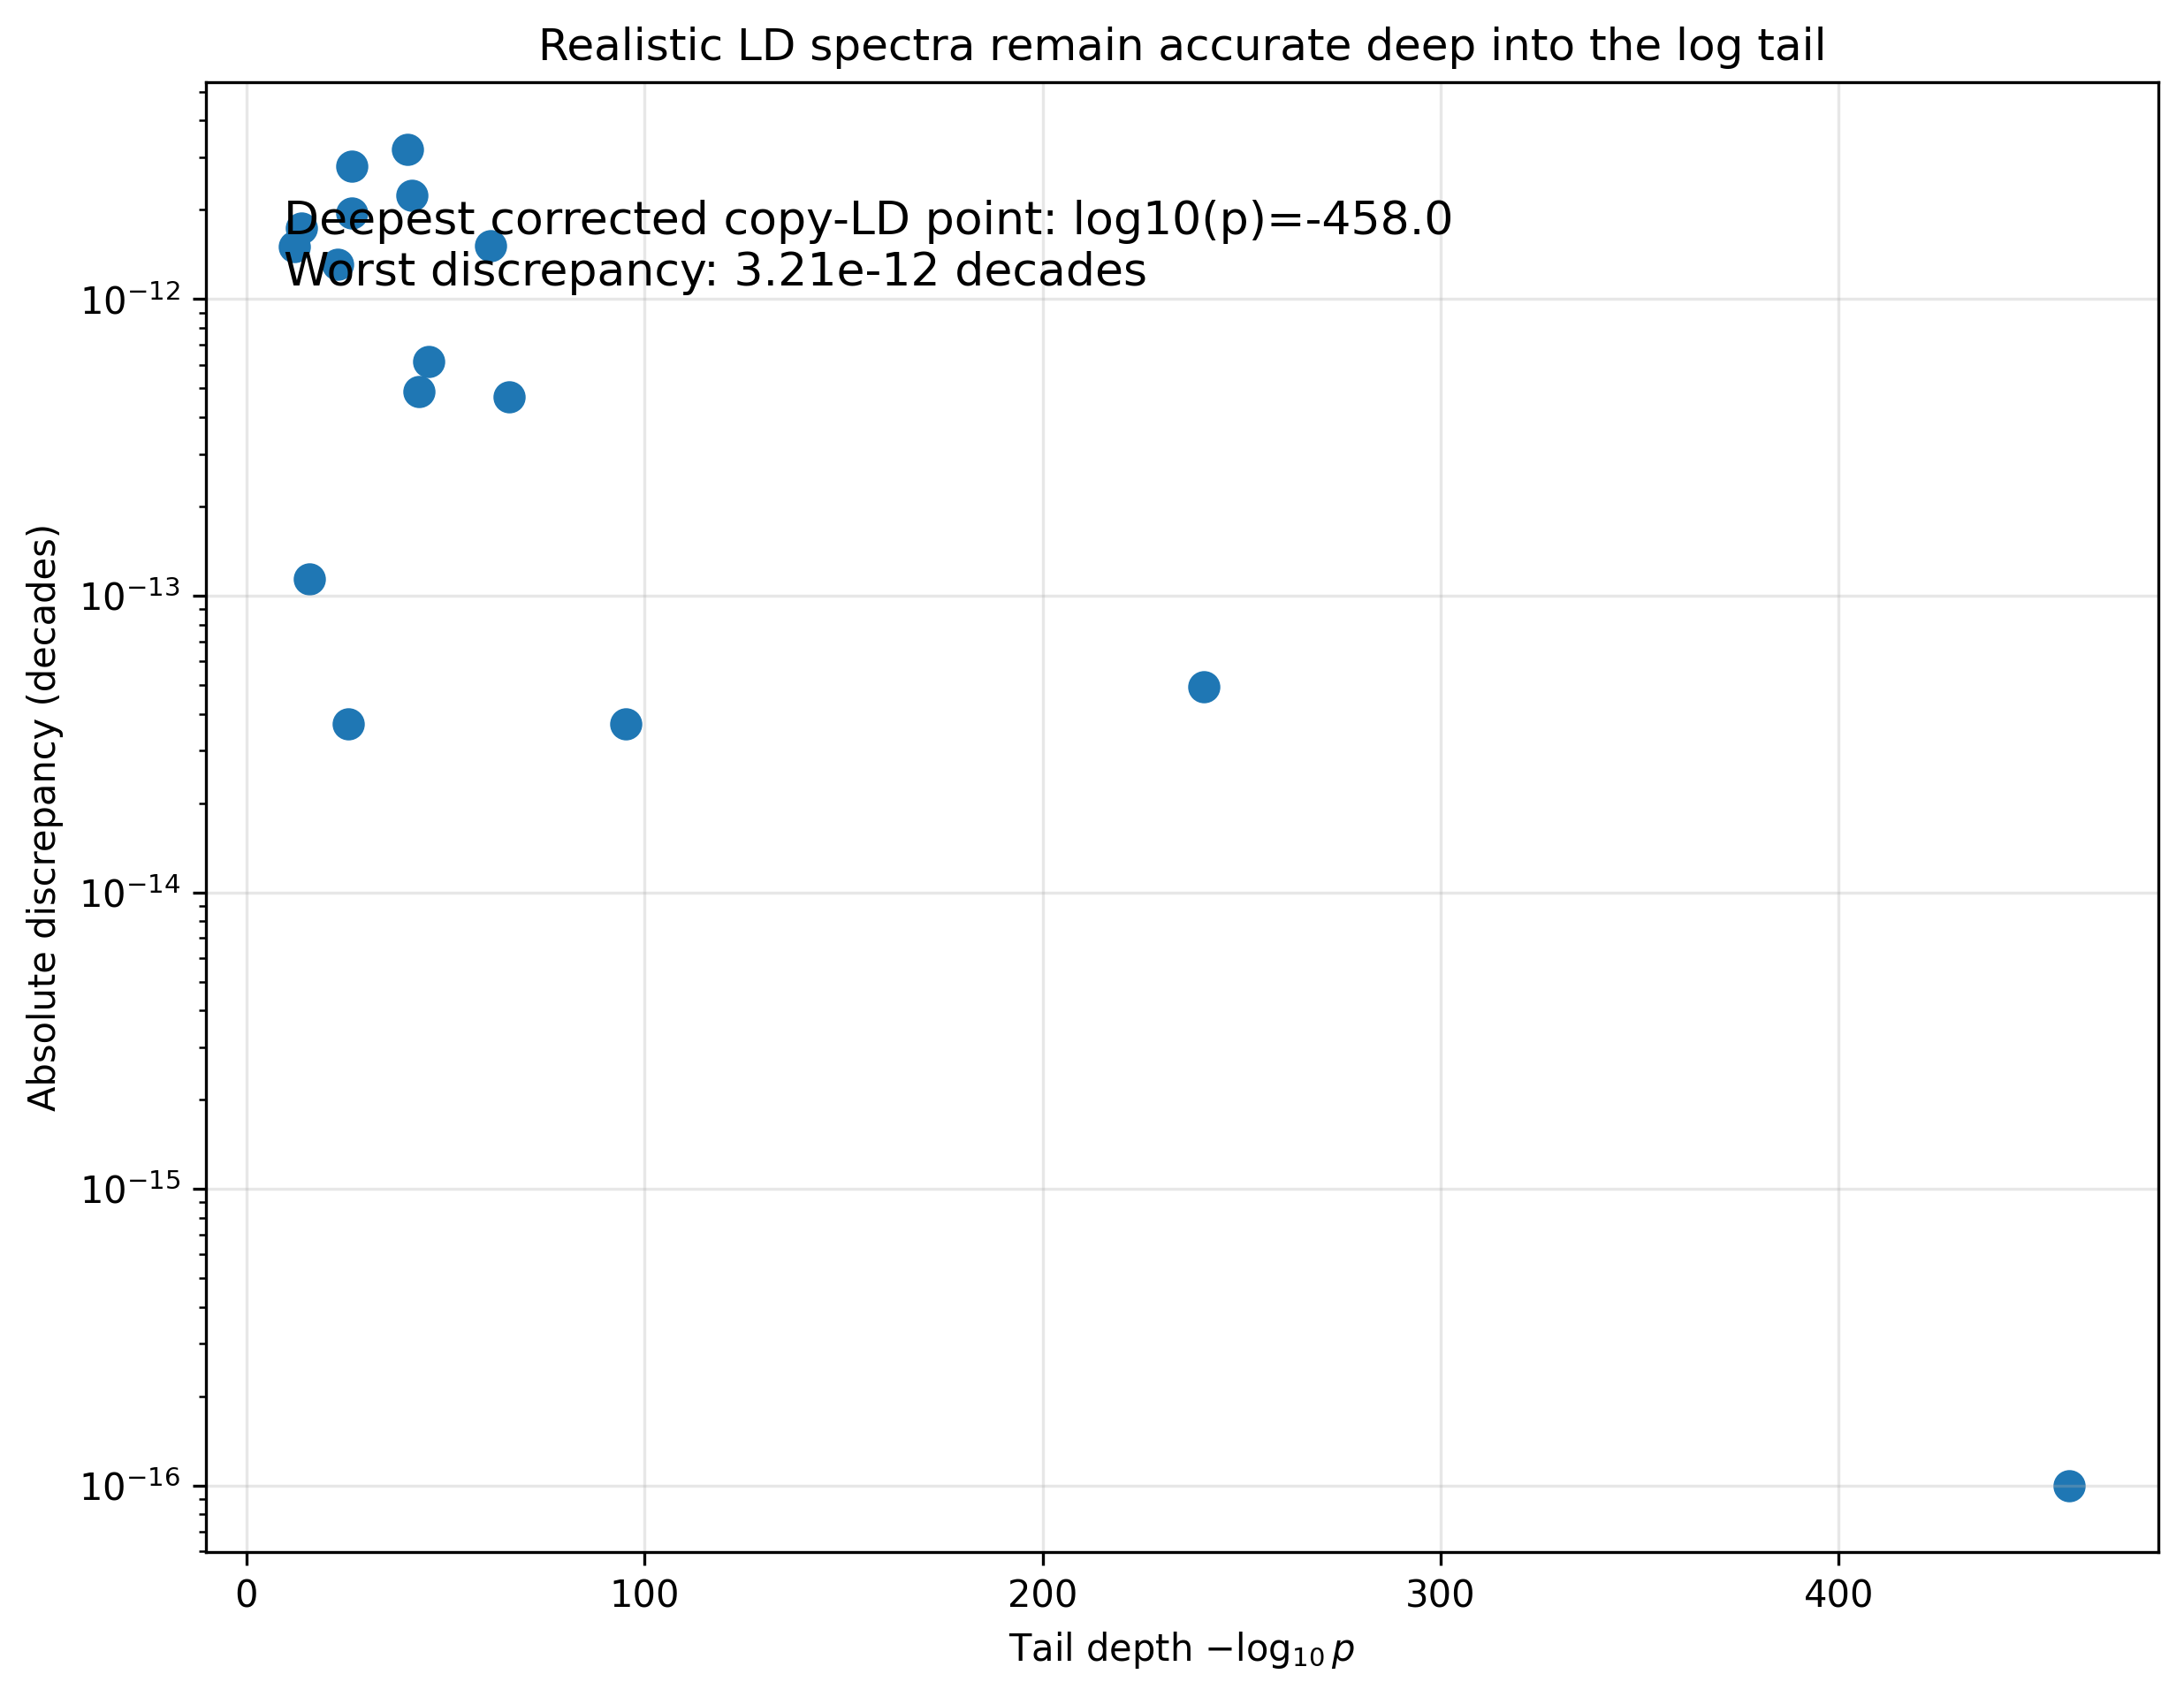
\includegraphics[width=.84\linewidth]{figure_20_realistic_deep_tail_accuracy.png}
\caption{K-COS versus the high-resolution full-spectrum tilted reference on
realistic LD spectra.  Accuracy remains at roughly machine-scale in log
probability through the deepest corrected copy-LD query, near $10^{-458}$.}
\label{fig:realistic-deep-tail}
\end{figure}

For the $n=1000$, $m=5000$ corrected copy-LD spectrum, selected results are

\begin{center}
\begin{tabular}{rrrr}
\toprule
tilt fraction & $\log_{10}p$ & K-COS $K$ & absolute error (decades)\\
\midrule
0.9950 & -65.950669 & 2048 & $4.69\times10^{-13}$\\
0.9970 & -95.305034 & 2048 & $3.70\times10^{-14}$\\
0.9990 & -240.602047 & 8192 & $4.94\times10^{-14}$\\
0.9995 & -457.973916 & 16384 & below displayed precision\\
\bottomrule
\end{tabular}
\end{center}

\subsection{Interpretation and boundary}

This simulation block does not add a new algebraic theorem.  It supplies a
more demanding validation layer for the theorem chain already proved.
Specifically, it shows that the exact streaming identities and the K-COS
deep-tail machinery remain numerically stable under substantially different
rare-variant LD structures and through the complete raw-genotype preprocessing
path.

The evidence remains synthetic.  These generators do not reproduce every
population-genetic feature of a sequencing cohort, and this block is not an
external-cohort replication.  It also addresses the Gaussian linear-model null;
finite-sample Bernoulli or logistic calibration remains a separate statistical
problem.


\section{Interface to spectral packets and K-COS}

The matrix packets above operate before eigendecomposition.  They should be
distinguished from the spectral packets used after the eigenvalues
\(\lambda_j\) are known.

The complete stack is
\[
\boxed{
\begin{aligned}
G
&\to \text{storage blocks}\\
&\to \text{matrix phases}\\
&\to \text{streamed }A,A^\top,K\\
&\to \text{polyphase/rank-adaptive Krylov}\\
&\to \text{small spectral core}\\
&\to \{\lambda_j\}\\
&\to \text{centered spectral packets}\\
&\to \text{deep-tail K-COS}.
\end{aligned}
}
\]

Storage decomposition, structural decomposition, spectral compression, and
tail compression are independent axes and can be active simultaneously.


\begin{figure}[H]
\centering
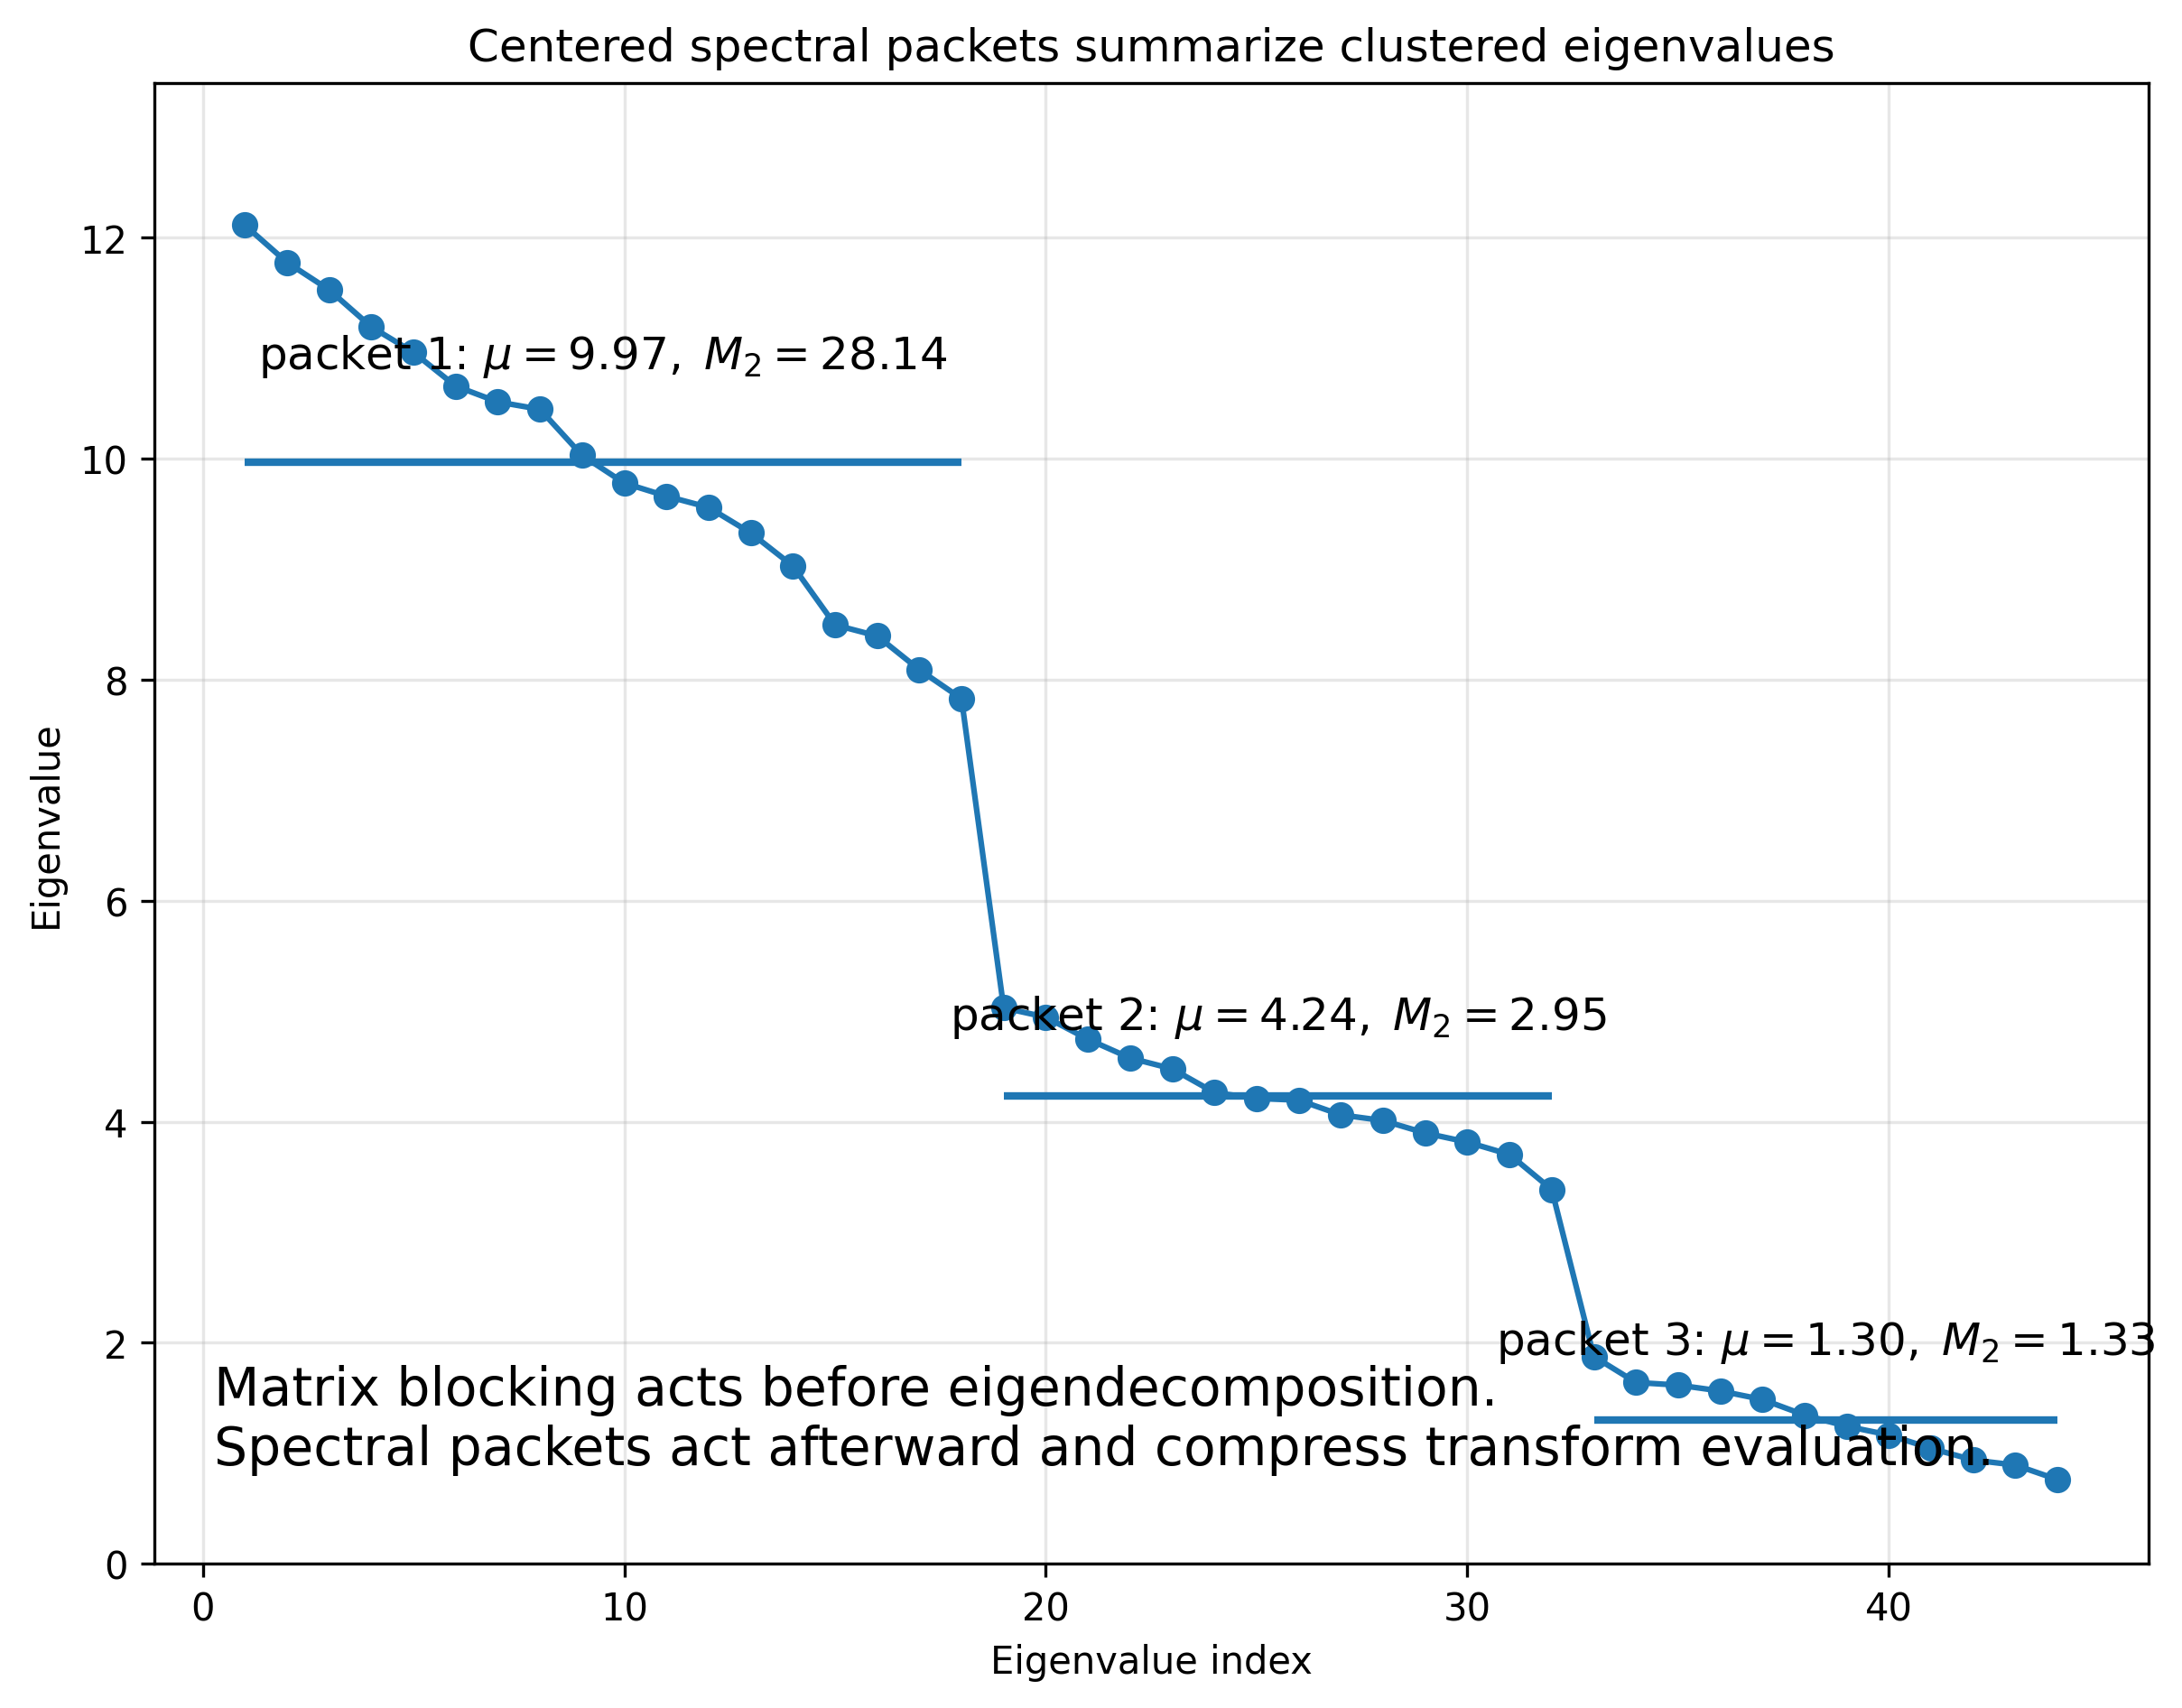
\includegraphics[width=.86\linewidth]{figure_07_spectral_packets.png}
\caption{Spectral packets form a second, distinct decomposition layer. After the large matrix problem has been reduced to eigenvalues, nearby eigenvalues are represented by packet centers and centered moments for K-COS transform evaluation. These spectral packets should not be confused with the storage blocks used before eigendecomposition.}
\label{fig:spectral-packets}
\end{figure}

\section{Memory planning law}

Let \(d\) be the number of bytes per floating scalar, \(c\) the resident
variant count, \(s\) the Krylov width, and \(p\) the covariate rank.
Ignoring library workspace and allocator overhead, a streamed sample-space
action has working memory on the order of
\[
\boxed{
d\,[nc+2ns+cs+np+O(ps+c)].
}
\]

The full factor costs
\[
dnm.
\]

For fixed \(n,p,s,c\),
\[
\boxed{
\frac{M_{\rm stream}}{M_{\rm full}}
=
O\!\left(
\frac{c}{m}
+
\frac{s}{m}
+
\frac{p}{m}
\right),
}
\]
so device memory remains bounded as total variant count grows.

\begin{table}[H]
\centering
\caption{Algebraic float64 memory model for \(n=2000\), \(p=4\),
Krylov width \(s=16\), resident variant block \(c=1024\).}
\begin{tabular}{rrrr}
\toprule
\(m\) & full factor (MiB) & streamed \(KV\) (MiB) & tiled Gram (MiB)\\
\midrule
10,000 & 152.6 & 16.308 & 8.555\\
50,000 & 762.9 & 16.308 & 8.555\\
100,000 & 1,525.9 & 16.308 & 8.555\\
500,000 & 7,629.4 & 16.308 & 8.555\\
1,000,000 & 15,258.8 & 16.308 & 8.555\\
\bottomrule
\end{tabular}
\end{table}


\begin{figure}[H]
\centering
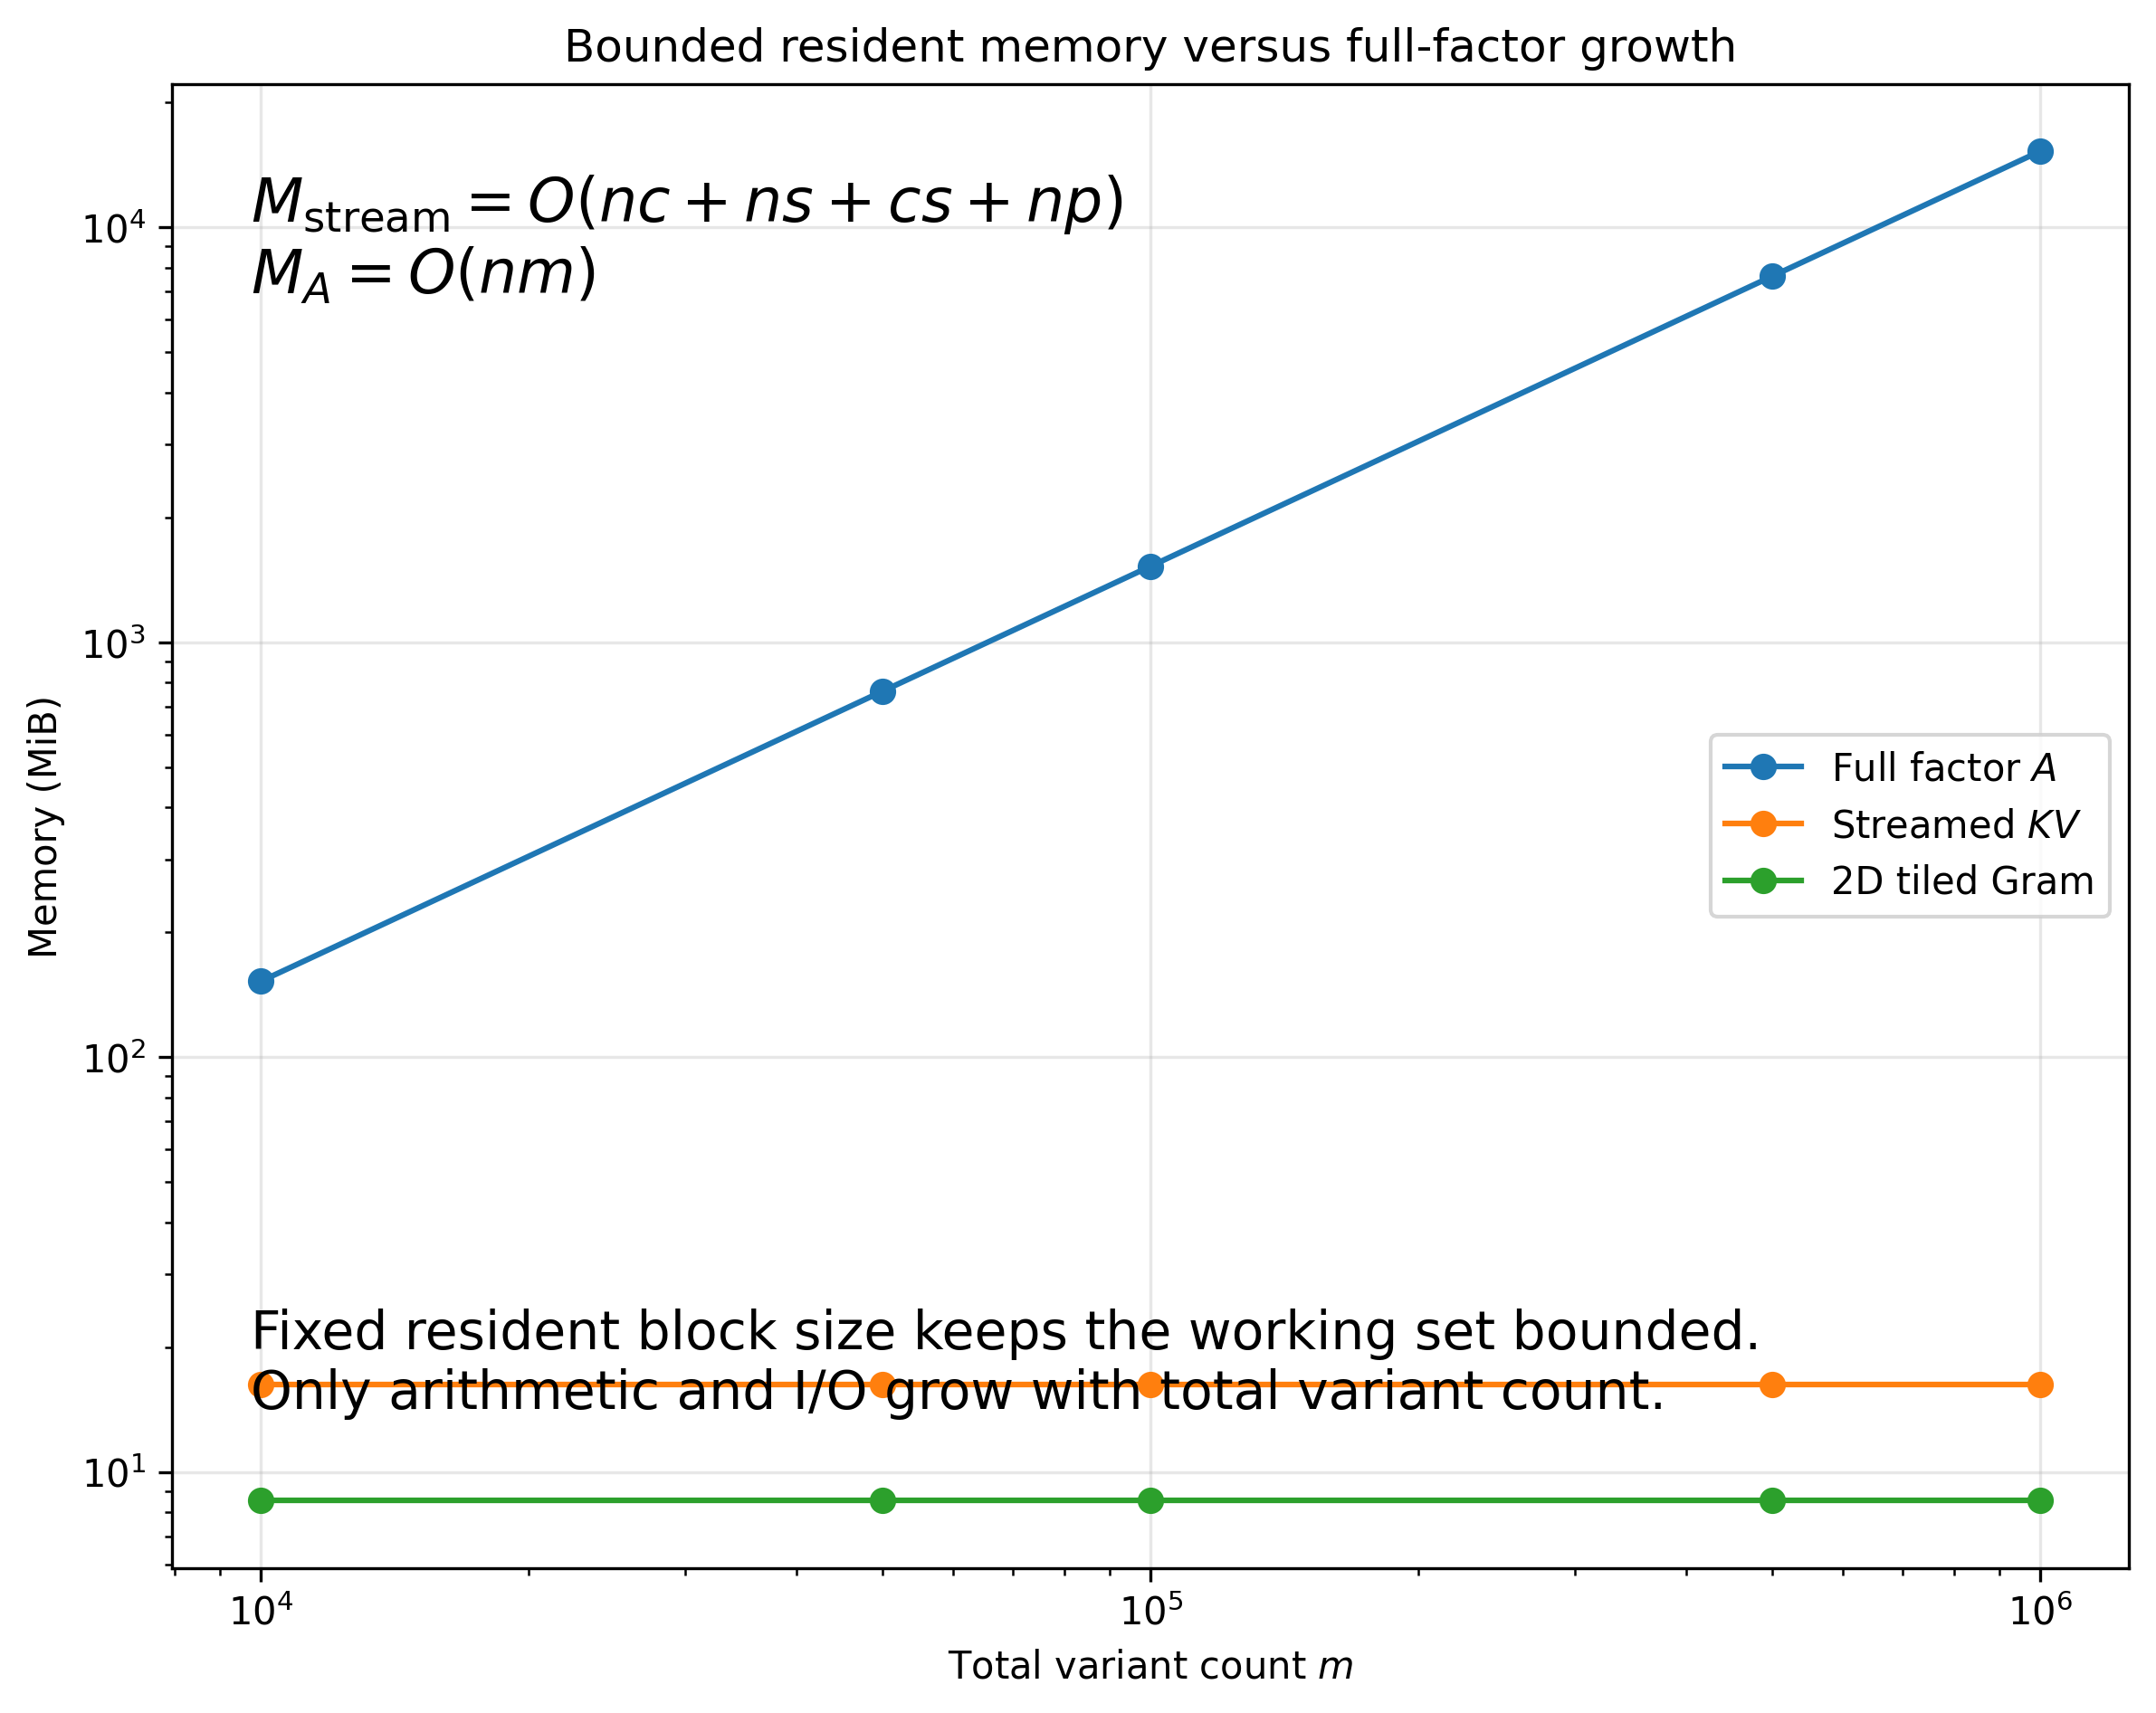
\includegraphics[width=.84\linewidth]{figure_03_memory_law.png}
\caption{The memory law. The complete factor grows linearly with total variant count $m$, whereas the streamed kernel action and the two-dimensional tiled construction remain bounded when resident block size, Krylov width, and covariate rank are fixed.}
\label{fig:memory-law}
\end{figure}

\section{Numerical verification}

All identities were compared against explicitly formed reference matrices.

\begin{table}[H]
\centering
\caption{Partition-invariance checks.}
\begin{tabular}{lrrr}
\toprule
partition & blocks & Gram relative error & action relative error\\
\midrule
coarse 4 & 4 & \(2.91\times10^{-16}\) & \(5.99\times10^{-16}\)\\
fine 64 & 32 & \(3.39\times10^{-16}\) & \(6.00\times10^{-16}\)\\
irregular & 9 & \(3.34\times10^{-16}\) & \(5.87\times10^{-16}\)\\
singleton-front & 21 & \(2.43\times10^{-16}\) & \(5.82\times10^{-16}\)\\
permuted, block 73 & 29 & \(3.52\times10^{-16}\) & \(5.89\times10^{-16}\)\\
\bottomrule
\end{tabular}
\end{table}

A hierarchical coarse-to-fine refinement gave relative discrepancy
\[
3.17\times10^{-16}.
\]

For an explicitly PSD polyphase operator
\[
H=L^\top L
\]
with block-bidiagonal \(L\), the smallest eigenvalue was approximately
\[
2.86,
\]
and the largest norm observed outside the exact \(k\)-step light cone was
\[
\boxed{0}.
\]

The QR-core update reproduced the full singular spectrum with relative
\(\ell_2\) discrepancy
\[
5.89\times10^{-16}.
\]


\section{A visual map of the decomposition calculus}

Figures~\ref{fig:residualization-geometry}--\ref{fig:partition-invariance} trace the mathematical object through its successive representations. Residualization first restricts the problem to the null-model orthogonal complement. Exact block-Gram additivity then permits memory-bounded streaming. Partition invariance separates physical storage granularity from the operator itself, while the phase graph constrains propagation through an exact light cone. Phase-local rank removes redundant basis directions; QR-core reuse preserves spectra under small updates; and spectral packets compress the final generalized-$\chi^2$ transform. The figures therefore represent a sequence of exact representation changes, each preserving the semantic object needed by the next layer.

\section{Solver portfolio}

\begin{longtable}{p{0.25\linewidth}p{0.30\linewidth}p{0.36\linewidth}}
\toprule
Regime & Preferred method & Reason\\
\midrule
factor fits comfortably & direct factor or sample Gram & lowest implementation overhead\\
factor exceeds device memory & streamed \(AV\), \(A^\top U\), or \(KV\) & exact memory-bounded execution\\
single block still too large & 2D sample/variant tiling & exact resident-tile bound\\
low numerical rank & block Golub--Kahan / range core & solve at rank scale\\
sparse exact phase graph & polyphase frontier Krylov & skip unreachable phases\\
nonuniform phase novelty & phase-local rank allocation & dimension-minimal exact width\\
low-rank phase interface & compressed message factors & reduce communication/storage\\
overlapping sets & QR-core update & exact reuse\\
full spectrum known & K-COS spectral packets & deep-tail transform compression\\
\bottomrule
\end{longtable}


\section{Relation to prior art and candidate novelty}

The individual numerical primitives used in this manuscript are not new in
isolation.  Blocked matrix multiplication, out-of-core linear algebra,
Lanczos and Golub--Kahan iteration, QR factorization, and low-rank operator
application are classical tools.  Randomized matrix approximation also has a
well-developed pass-efficient and streaming literature; in particular,
Halko, Martinsson, and Tropp describe algorithms intended for matrices too
large to fit in fast memory and emphasize constant-pass or single-pass
approaches \cite{Halko2011}.  In the SKAT literature, fastSKAT specifically
uses randomized projection and Lanczos-type ideas to avoid a complete dense
eigendecomposition, computing leading eigenvalues and approximating the
remaining spectral contribution \cite{Lumley2018}.  The original SKAT
framework and its weighted quadratic-form null distribution are due to Wu
et al. \cite{Wu2011}.

Accordingly, the contribution claimed here is \emph{not} the invention of
blocking, streaming, matrix-free multiplication, or Krylov iteration.  The
candidate contribution is the exact composition of four independent
representations:
\[
\boxed{
\mathcal D
=
\mathcal D_{\rm storage}
\circ
\mathcal D_{\rm phase}
\circ
\mathcal D_{\rm rank}
\circ
\mathcal D_{\rm spectrum}.
}
\]
The first controls device residency, the second controls structural
propagation, the third controls spectral dimension, and the fourth controls
deep-tail transform cost.

\subsection{Storage-phase commutation}

Fix a structural phase partition
\[
\{1,\ldots,m\}=\mathcal P_1\sqcup\cdots\sqcup\mathcal P_H
\]
and let each phase be subdivided into arbitrary storage blocks
\[
\mathcal P_h
=
J_{h1}\sqcup\cdots\sqcup J_{hB_h}.
\]
Let $S$ denote this physical storage subdivision.  The phase projectors
$P_h$ are defined by the structural phases, not by $S$.

\begin{theorem}[Storage-phase commutation theorem]
Let
\[
A=M_XGW^{1/2},
\qquad H=A^\top A,
\]
and let $S$ and $S'$ be any two exact storage refinements that respect the
same structural phase partition.  Then:
\begin{enumerate}[label=(\roman*)]
\item the exact operator $H$ is identical under $S$ and $S'$;
\item every phase coupling $P_hHP_g$ is identical under $S$ and $S'$;
\item the exact phase graph and every $k$-step polyphase light cone are
identical under $S$ and $S'$;
\item any exact matrix-free Krylov method applied through streamed products
produces the same Krylov subspaces in exact arithmetic under $S$ and $S'$.
\end{enumerate}
\end{theorem}

\begin{proof}
Storage refinement changes only the order and grouping of finite sums.
By partition refinement invariance, the streamed products reconstruct the
same $A$, $A^\top$, and therefore the same $H=A^\top A$.  Since each
$P_h$ is fixed by the structural phase partition, every block
$P_hHP_g$ is unchanged.  The phase graph is defined only by these blocks, so
its path structure and light cones are unchanged.  Finally, an exact
matrix-free Krylov method depends only on repeated applications of the same
operator to the same starting block; hence its generated subspaces are
identical.
\end{proof}

\begin{corollary}[Adaptive resident-block scheduler]
An implementation may change resident block size at runtime---including
recursively splitting a phase block after an allocation failure---without
changing the exact phase graph or exact Krylov trajectory, provided all
required storage blocks are processed exactly.
\end{corollary}

This separates \emph{mathematical locality} from \emph{physical storage
granularity}.  A phase may remain fixed as an LD window or annotation class
while its physical representation is subdivided according to free GPU
memory, scalar precision, transfer granularity, or stream count.

\subsection{Frontier-to-I/O theorem}

\begin{theorem}[Exact frontier-to-I/O reduction]
Suppose the exact phase graph of $H$ is used and the current Krylov block is
supported on a phase set $F_0$.  At depth $k$, let $F_k$ be the graph
$k$-neighborhood of $F_0$.  Then no storage block lying wholly in a phase
outside $F_k$ can affect the $k$-step Krylov vector.  Such a block need not be
loaded during that step.
\end{theorem}

\begin{proof}
For every phase $h\notin F_k$ and every starting phase $g\in F_0$, the
polyphase light-cone theorem gives $P_hH^kP_g=0$.  Storage-phase commutation
allows each active phase operator to be evaluated through arbitrary exact
storage blocks.  Therefore blocks outside the active structural frontier
contribute identically zero to the requested iterate and may be omitted.
\end{proof}

The theorem turns an algebraic support statement into an execution law:
\[
\boxed{
\text{Krylov depth}
\longrightarrow
\text{reachable phases}
\longrightarrow
\text{storage blocks that must be transferred}.
}
\]
This is stronger than ordinary chunking, because the scheduler is constrained
by the exact operator graph rather than solely by available memory.

\subsection{Comparison with fastSKAT}

fastSKAT attacks the same broad spectral bottleneck but follows a different
approximation strategy: it computes leading eigenvalues using randomized or
Lanczos-type methods and approximates the remainder of the quadratic-form
spectrum \cite{Lumley2018}.  The present architecture instead separates
memory blocking from structural propagation and can continue, when desired,
to exact range capture and an explicit small spectral core before handing the
resulting eigenvalues to a separate deep-tail engine.  Thus the strongest
novelty claim is not ``matrix-free SKAT,'' which is prior art, but the
storage-invariant polyphase scheduler and its composition with local-rank,
core-reuse, and tail-packet layers.

\subsection{Novelty statement and boundary}

A targeted literature review conducted for this manuscript identified prior
work on SKAT, fastSKAT, out-of-core randomized matrix decompositions, and
classical Krylov solvers, but did not identify a SKAT solver that combines all
of the following in one exact architecture:
\begin{enumerate}
\item residualization-preserving streamed factor actions;
\item storage refinement invariant under runtime block subdivision;
\item an exact structural phase graph with finite-step light cones;
\item phase-local minimal Krylov width;
\item low-rank inter-phase messages and exact QR-core update reuse;
\item an explicit transition from the small spectral core to a separately
certified deep-tail spectral-packet calculation.
\end{enumerate}
This absence is evidence for a candidate systems/methodological contribution,
not a proof of global novelty.  The appropriate publication claim is that the
\emph{composition and its exact invariance laws appear to be novel}, while
its numerical primitives are classical.

\section{Claim boundary}

The manuscript deliberately uses a narrow novelty boundary. Blocking, tiled matrix multiplication, out-of-core linear algebra, randomized low-rank approximation, Golub--Kahan/Lanczos iteration, QR, and low-rank factor application are inherited techniques \cite{Halko2011,Lumley2018}. The contribution should not be stated as the invention of blocking or matrix-free SKAT.

The candidate Komorebi contribution is the resolved synthesis
\[
\boxed{\begin{aligned}
&\text{exact streamed factor actions}
+\text{ polyphase light cones}
+\text{ minimal phase rank}\\
&+\text{ low-rank messages}
+\text{ exact update cores}
+\text{ deep-tail spectral packets}.
\end{aligned}}
\]

The conceptual claim is that storage decomposition, structural phase
decomposition, spectral compression, and tail compression are mathematically
distinct layers and can be composed without changing the exact operator.

\section{Current proof and validation ledger}

\small
\begin{tabular}{p{0.46\linewidth}p{0.18\linewidth}p{0.26\linewidth}}
\toprule
Item & Status & Evidence\\
\midrule
block Gram additivity & proved & direct matrix identity\\
streamed \(KV\) & proved & direct matrix identity\\
streamed \(AV,A^\top U\) & proved & factor partition\\
2D tiling & proved & row-block expansion\\
partition refinement invariance & proved & disjoint-union argument\\
variant permutation invariance & proved & simultaneous coordinate permutation\\
storage-phase commutation & proved & operator invariance under storage refinement\\
frontier-to-I/O reduction & proved & light-cone support plus storage commutation\\
polyphase light cone & proved & projector-path expansion\\
minimal phase width & proved & dimension argument\\
QR-core update & proved & orthonormal left factor\\
range-core spectrum & proved & singular-value invariance\\
machine-precision implementation & tested & explicit-reference comparisons\\
GPU wall-clock crossover & open & requires production CUDA implementation\\
I/O-optimal scheduling & open & hardware/backing-store dependent\\
approximate phase graph error bound & proved/tested & weighted transfer matrix and thresholded-power certificate\\
budget-optimal equal-cost scheduler & proved/tested & additive edge-risk theorem plus exhaustive audit\\
unequal-cost scheduler & formulated/tested & certified knapsack heuristic with fractional upper bound\\
double-buffer pipeline model & proved/model only & ideal asynchronous-overlap proposition\\
trace-aware residual MGF envelope & proved/tested & exact residual decomposition plus trace--Frobenius--cap bound\\
residual-rank moment bracket & proved/tested & trace/cap and trace-square rank inequalities\\
streamed residual completion & proved/tested & orthogonal residual factor and incremental completion core\\
\bottomrule
\end{tabular}
\normalsize

\section{Next formal targets}

The next blocks should address:

\begin{enumerate}
\item integrate the hybrid Krylov/moment/completion stopping rule into the
production K-COS API;
\item implement rank-revealing residual completion with fused GPU block QR or
TSQR rather than the reference SVD path;
\item derive randomized or block-Krylov convergence bounds under streamed,
phase-pruned actions;
\item benchmark the complete scheduler on native GPU hardware, including
PCIe overlap, allocator workspace, and block-size crossover.
\end{enumerate}

\appendix

\section{Reference pseudocode}

\begin{lstlisting}[language=Python]
def stream_KV(block_source, weights, Qx, V):
    U = V - Qx @ (Qx.T @ V)
    Y = zeros_like(U)
    for G_block, w_block in block_source:
        T = G_block.T @ U
        Y += G_block @ (w_block[:, None] * T)
    return Y - Qx @ (Qx.T @ Y)
\end{lstlisting}

\section{Running manuscript protocol}

This file is intended to remain cumulative.  New theorem blocks should be
added with one of three labels:

\begin{itemize}
\item \textbf{proved}: a complete mathematical argument is present;
\item \textbf{validated}: a numerical experiment supports the statement but
does not prove it;
\item \textbf{open}: the obstruction or missing assumption is recorded.
\end{itemize}

Negative timings, failed approximations, and counterexamples should be retained
in the running ledger rather than removed from later versions.


\begin{thebibliography}{9}

\bibitem{Wu2011}
M. C. Wu, S. Lee, T. Cai, Y. Li, M. Boehnke, and X. Lin,
``Rare-Variant Association Testing for Sequencing Data with the Sequence
Kernel Association Test,''
\emph{American Journal of Human Genetics}, 89(1):82--93, 2011.
DOI: 10.1016/j.ajhg.2011.05.029.

\bibitem{Halko2011}
N. Halko, P. G. Martinsson, and J. A. Tropp,
``Finding Structure with Randomness: Probabilistic Algorithms for Constructing
Approximate Matrix Decompositions,''
\emph{SIAM Review}, 53(2):217--288, 2011.
DOI: 10.1137/090771806.

\bibitem{Lumley2018}
T. Lumley, J. Brody, G. Peloso, A. Morrison, and K. Rice,
``FastSKAT: Sequence Kernel Association Tests for Very Large Sets of Markers,''
\emph{Genetic Epidemiology}, 2018.
PMCID: PMC6129408.

\end{thebibliography}

\end{document}
